%% LyX 2.1.3 created this file.  For more info, see http://www.lyx.org/.
%% Do not edit unless you really know what you are doing.
\documentclass[12pt,oneside,english,reqno]{amsbook}
\renewcommand{\familydefault}{\rmdefault}
\usepackage[T1]{fontenc}
\usepackage[latin9]{inputenc}
\usepackage{geometry}
\geometry{verbose,tmargin=1in,bmargin=1in,lmargin=1in,rmargin=1in}
\usepackage{mathrsfs}
\usepackage{url}
\usepackage{amsthm}
\usepackage{amstext}
\usepackage{stmaryrd}
\usepackage{graphicx}
\usepackage{setspace}
\doublespacing

\makeatletter

%%%%%%%%%%%%%%%%%%%%%%%%%%%%%% LyX specific LaTeX commands.
%% A simple dot to overcome graphicx limitations
\newcommand{\lyxdot}{.}
%%%%%%%

 \newcommand{\abs}[1]{\left|{#1}\right|}
 \newcommand{\av}[1]{\left\langle #1 \right\rangle}
 
  \newcommand{\br}[1]{\langle #1|}
  \newcommand{\ke}[1]{|#1\rangle}
  \newcommand{\bk}[2]{\langle #1|#2\rangle}
  \newcommand{\kb}[2]{\ke{#1}\br{#2}}
  \newcommand{\var}[2]{\langle #1,#2\rangle} 
  
  \newcommand{\al}[1]{^{(#1)}}
  \newcommand{\da}{^\dagger} 
  
  \newcommand{\pt}[1]{\left( #1 \right)}
  \newcommand{\pq}[1]{\left[ #1 \right]}
  \newcommand{\pg}[1]{\left\{ #1 \right\}} 
  
  \newcommand{\lpt}[1]{\left( #1 \right.}
  \newcommand{\lpq}[1]{\left[ #1 \right.]}
  \newcommand{\lpg}[1]{\left\{ #1 \right.}
  \newcommand{\rpt}[1]{\left. #1 \right)}
  \newcommand{\rpq}[1]{\left. #1 \right]}
  \newcommand{\rpg}[1]{\left. #1 \right\}} 


\newcommand{\td}[1]{\widetilde{#1}}

%%%%%%%%%%%%%%%%%%%%%%%%%%%%%% Textclass specific LaTeX commands.
\numberwithin{section}{chapter}
\numberwithin{equation}{section}
\numberwithin{figure}{section}

\makeatother

\usepackage{babel}
\begin{document}


\global\long\def\sandwich#1#2#3{ \left\langle #1\left|#2\right|#3\right\rangle }
\global\long\def\ket#1{\left|#1\right>}
\global\long\def\braket#1#2{\left\langle #1\mid#2\right\rangle }
\global\long\def\bra#1{\left\langle #1\right|}
\global\long\def\indep{\perp\!\!\!\perp}




 \thispagestyle{empty}\pagenumbering{gobble}

\vphantom{}

\textbf{\large{}Quantum State Discrimination and Quantum Cloning: }{\large \par}

\textbf{\large{}\hspace{2.7cm}Optimization and Implementation }{\large \par}

\vspace{1.2cm}


{\huge{}\hspace{5cm}\hspace{1cm}\hspace{1cm}}by

\vspace{0.7cm}


{\huge{}\hspace{5cm}\hspace{1.1cm}}Lazy bum

\vfill{}


\begin{singlespace}
A dissertation submitted to the Graduate Faculty in Physics in partial
fulfillment of the requirements for the degree of Doctor of Philosophy,
The City University of New York 
\end{singlespace}

\begin{center}
2015
\par\end{center}

\pagebreak{}

 \pagenumbering{roman}\setcounter{page}{2}\vphantom{}

\begin{singlespace}
\begin{center}
\vfill{}

\par\end{center}

%\begin{center}
%\includegraphics[width=2cm]{../ugur_dissertation_copy/img/creative_commons_logo_by}
%\par\end{center}

\begin{center}
2015\\
Undeserving lazy bum\\
Some rights reserved.\\
This work is licensed under a Creative Commons\\
Attribution 4.0 United States License.\\
\url{http://creativecommons.org/licenses/by/4.0/}
\par\end{center}
\end{singlespace}

\pagebreak{}

\vphantom{}

\vfill{}


\begin{center}
\begin{minipage}[c][1\totalheight][t]{1\columnwidth}%
\begin{singlespace}
\begin{center}
This manuscript has been read and accepted for the\\
Graduate Faculty in Physics in satisfaction of the \\
dissertation requirement for the degree of Doctor of Philosophy.
\par\end{center}\end{singlespace}
%
\end{minipage}
\par\end{center}

\vspace{3cm}


\begin{minipage}[t]{0.25\columnwidth}%
\begin{singlespace}
\rule[0.5ex]{1\columnwidth}{1pt}

Date\end{singlespace}
%
\end{minipage} \hfill{}%
\begin{minipage}[t]{0.6\columnwidth}%
\begin{singlespace}
\rule[0.5ex]{1\columnwidth}{1pt}

Prof. J�nos A. Bergou

Chair of Examining Committee\end{singlespace}
%
\end{minipage}

\vspace{2cm}


\begin{minipage}[t]{0.25\columnwidth}%
\begin{singlespace}
\rule[0.5ex]{1\columnwidth}{1pt}

Date\end{singlespace}
%
\end{minipage} \hfill{}%
\begin{minipage}[t]{0.6\columnwidth}%
\begin{singlespace}
\rule[0.5ex]{1\columnwidth}{1pt}

Prof. Igor L. Kuskovsky

Executive Officer\end{singlespace}
%
\end{minipage}

\vspace{1.5cm}


\begin{center}
\begin{minipage}[t]{0.8\columnwidth}%
\begin{singlespace}
Supervisory Committee:

\vspace{1cm}


Prof. Mark Hillery\hfill{}

\vspace{1cm}


Prof. Steven Greenbaum\hfill{} 

\vspace{1cm}


Prof. Ed Feldman\hfill{}

\vspace{1cm}


Prof. Neepa T. Maitra\hfill{}\end{singlespace}
%
\end{minipage}
\par\end{center}

\vspace{0.5cm}


\begin{center}
THE CITY UNIVERSITY OF NEW YORK
\par\end{center}

\pagebreak{}

{\huge{}\hspace{5cm}\hspace{1.2cm}}\textbf{\Large{}Abstract}{\Large \par}

\vspace{1.5cm}


\textbf{\large{}Quantum State Discrimination and Quantum Cloning: }{\large \par}

\textbf{\large{}\hspace{2.7cm}Optimization and Implementation }{\large \par}

\vspace{1.2cm}


{\huge{}\hspace{5cm}\hspace{1cm}\hspace{1cm}}by

\vspace{0.7cm}


{\huge{}\hspace{5cm}\hspace{1.1cm}}Lazy Bum

\vspace{1cm}


\textbf{Advisor:}\textbf{\small{} }Janos A. Bergou

\vspace{1cm}

This thesis reflects works previously published by the author and materials 
hitherto unpublished on the subject of quantum information theory.  Particularly,
results in optimal discrimination, cloning, and separation of quantum states, 
and their relationships, are discussed.  Via Neumark's theorem \cite{Neumark}, 
our description of these unitary processes can be implemented with linear optical devices. 



















In our work we explore the field of quantum state discrimination and
quantum cloning. Recently the problem of optimal state discrimination
with a Fixed Rate of Inconclusive Outcomes (FRIO strategy) has been
solved for two pure quantum states and a few other highly symmetric
cases. An optical implementation to FRIO for pure states is provided.
The physical implementation can be carried out with the use of a six-port
interferometer constructed with optical fibers beam splitters, phase
shifters and mirrors. The input states are composed of qubits which
are realized as photons in the dual-rail representation. The non-unitary
measurements are carried out at the output for the presence or absence
of a photon. The setup optimally interpolates between minimum error
and unambiguous state discrimination. We also extend the FRIO strategy
to two mixed states, whose eigenvectors in their spectral representation
form a Jordan basis. We derive the minimum error rate $P_{E}$ for
a fixed inconclusive rate $Q$ and, in particular, the optimal distribution
of the total $Q$ over the Jordan subspaces. As $Q$ is varied between
the two limits, $0<Q<Q_{c}$, a structure with multiple thresholds,
$Q_{1}^{(th)}(=0)<Q_{2}^{(th)}<\ldots<Q_{N}^{(th)}<Q_{c}$, emerges.
We also solve the problem of state separation of two known pure states
in the general case where the known states have arbitrary prior probabilities.
The solution emerges from a geometric formulation of the problem.
This formulation also reveals a deeper connection between cloning
and state discrimination. The results are then applied in designing
a scheme for hybrid cloning which interpolates between approximate
and probabilistic exact cloning. It is shown that state separation
and hybrid cloning are generalized schemes to well established state
discrimination and cloning strategies. The relationships between cloning,
state separation and state discrimination are derived in several limints. 



{\huge{}\hspace{1.0cm}}\textbf{\Large{}}{\Large \par}

\vspace{1.5cm}

\vspace{1.2cm}

\chapter*{Acknowledgements}


\vspace{0.7cm}



\vspace{1cm}


THANKS BRUVS, MUCH LOVE!



\tableofcontents{}

\listoffigures


 \pagenumbering{arabic}\pagebreak{}

%%%%%%%%%%%%%%%%%%%%%%%%%%%%%%%%%%%%%%%%%%%%%%%%
%%%%%%%%%%%%%%%%%%%%%%%%%%%%%%%%%%%%%%%%%%%%%%%%
\chapter{Introduction}



\section{Properties of Measurement Theory}



Classical bits versus quantum bits: instead of just a 0 or 1, quantum bits can maintain a superposition state

The probabalistic nature of detection: only orthogonal states can be discriminated perfectly


Quantum Computing

Quantum Communication
 factorization work of Peter Schor \cite{Shor1994} and quantum
key distribution protocols such as B92 \cite{Bennett1992}. 

%%%%%%%%%%%%%%%%%%%%%%%%%%%%%%%%%%%%%%%%%%%%%%%%
%%%%%%%%%%%%%%%%%%%%%%%%%%%%%%%%%%%%%%%%%%%%%%%%
\section{State Representation and Measurements }

We begin by describing pure quantum states $\psi$ as vectors in a Hilbert space and an ensemble of states as
 $\rho  = \sum_i \eta_i \kb{\psi_ i}{\psi_i}$ where $\sum \eta_i = 1$. The evolution of this ensemble is the 
Schrodinger equation as
\[i \hbar \frac{\delta\rho}{\delta t} =  [H,\rho].\]
Solving this for time-independent evolution we get
\[\rho(t) = U(t) \rho(0) U(t)^\dagger.\]
and where the unitary matrix U obeys $UU^\dagger = I$.
There are several ways to view this formula. The first is by decomposing the unitary into a set of Kraus operators $A_i$
such that $U(\ke {\psi_A} \otimes \ke {\phi_B}) = \sum_i A_i \ke {\psi_A} \otimes \ke {i_B}$ and $\sum A_i A_i^\dagger = I$.
 The alternative effects of the evolution, for example a particle striking 
one detector as opposed to another, are described by the different operators $A_i$.  Blah blah measurement operators $\Pi_i$.

The other is due to Neumark \cite{Neumark1}. A unitary acts on a pure state $\psi$ to make state $\phi$, as in $U\ke \psi = \phi$.

Before we describe such processes particularly let us describe the mathematics of these structures.  The ensemble 
previously described can be describes as a density matrix.  This is a generalized state that is a statistical collection 
of pure states defined by four properties:

\begin{enumerate}
\item $\rho  = \sum_i \eta_i \kb{\psi_ i}{\psi_i}$ where $\sum \eta_i = 1$,
\item It is Hermitian ,
\item $Tr \rho = 1$,
\item $\br {\phi_i} \rho \ke {\phi_i} \geq 0$.
\end{enumerate}

The measurements $\Pi_i$ are a decomposition of the identity in terms of positive semi-definite matrices. 
A measurement can be either a projector onto an eigenvector of the Hilbert space or a generalized measurement.  In the latter case it must fulfill only 2 properties:

\begin{enumerate}
\item $\sum \Pi_i = 1$
\item They are Hermitian.  This corresponds to real eigenvalues (measurement outcomes).
\end{enumerate}

Since non-orthogonal states cannot be discriminated perfectly, we can speak of the probability of a given outcome:
	$\av {\Pi_i} = \sum_j \eta_j \br {\psi_j} \Pi_i \ke {\psi_j} = Tr(\Pi_i \rho)$


The generalization of the postulates of quantum mechanics in terms
of the POVM can be expressed as:
\begin{enumerate}
\item The decomposition of the identity in terms of positive operators,
$\Pi_{j}\geq0$, $\sum_{j}\Pi_{j}=I$ is called a POVM.
\item The elements of the POVM can be expressed in terms of the detection
operators $\Pi_{j}=A_{j}^{\dagger}A_{j}$ where the operators satisfy
the requirements $\sum_{j}A_{j}^{\dagger}A_{j}=I$ but they need not
be Hermitian.
\item A detection yields an element on POVM.
\item The state of the system collapses onto: $\ket{\phi_{j}}=\frac{A_{j}\ket{\psi}}{\sqrt{\sandwich{\psi}{A_{j}^{\dagger}A_{j}}{\psi}}}$
if the system was initially in a pure state, $\rho_{j}=\frac{A_{j}^{\dagger}\rho A_{j}}{Tr(A_{j}\rho A_{j}^{\dagger})}=\frac{A_{j}^{\dagger}\rho A_{j}}{Tr(A_{j}^{\dagger}A_{j}\rho)}=\frac{A_{j}^{\dagger}\rho A_{j}}{Tr(\Pi_{j}\rho)}$
if the system was initially in a mixed state. 
\item The probability of obtaining $\rho_{j}$ is $p_{j}=Tr(A_{j}\rho_{j}A_{j}^{\dagger})=Tr(A_{j}^{\dagger}A_{j}\rho_{j})=Tr(\Pi_{j}\rho_{j})$.
\item If a measurement is performed but the result is not recorded the post-measurement
state collapses onto: $\tilde{\rho}=\sum_{j}p_{j}\rho_{j}=\sum_{j}A_{j}\rho A_{j}^{\dagger}$.
\end{enumerate}
\subsection{Standard Quantum Measurements}

We start with the postulates of standard or projective quantum measurements
introduced by von Neumann \cite{Neumann1955} analyzing a model for
the coupling of the system with the meter or ancilla and generalizing
the predictions of the model. 

The postulates are:
\begin{enumerate}
\item Observables in quantum mechanics have a Hermintian operator $\chi$
which has a spectral representation $\chi=\sum_{j}^{N}\lambda_{j}\ket j\bra j$,
where the eigenvalues are real and assuming non-degeneracy for simplicity.
The eigenvectors $\left\{ \ket j\right\} $ form a complete orthonormal
basis set.
\item The Hilbert space is spanned by the projectors $P_{j}=\ket j\bra j$,
such that $\sum_{j}P_{j}=1.$ 
\item The eigenvalues of the projectors are $0$ or $1$ due to the orthogonality
of the states $P_{i}P_{j}=P_{i}\delta_{ij}$.
\item Any measurement of the $\chi$ will yield one of the eigenvalues $\lambda_{j}$.
\item If $\lambda_{j}$ is obtained in a measurements, the state of the
system collapses onto: $\ket{\phi_{j}}=\frac{P_{j}\ket{\psi}}{\sqrt{\sandwich{\psi}{P_{j}}{\psi}}}$
if the system was initially in a pure state, $\rho_{j}=\frac{P_{j}\rho P_{j}}{Tr(P_{j}\rho)}$
if the system was initially in a mixed state. 
\item The probability of obtaining $\ket{\phi_{j}}$ is $p_{j}=\left|\left|P_{j}\psi\right|\right|^{2}=\sandwich{\psi}{P_{j}^{2}}{\psi}=\sandwich{\psi}{P_{j}}{\psi}$.
The probability of obtaining $\rho_{j}$ is $p_{j}=Tr(P_{j}\rho P_{j})=Tr(P_{j}^{2}\rho)=Tr(P_{j}\rho)$. 
\item If a measurement is performed but the result is not recorded the post-measurement
state collapses onto: $\rho=\sum_{j}P_{j}\ket{\psi}\bra{\psi}P_{j}$
if the system was initially in a pure state, $\tilde{\rho}=\sum_{j}p_{j}\rho_{j}=\sum_{j}P_{j}\rho P_{j}$
if the system was initially in a mixed state.
\end{enumerate}

*************THIS NEEDS TO GO OR BE CHANGED**********************





An integral part of quantum information and quantum processing is
measurement theory \cite{Bergou2013}, the state is not an observable in quantum
mechanics \cite{Peres1995}. When a quantum circuit or processor has
acted on the input states to perform a task, the output needs to be
read out. Thus after the processing occurs the task is to determine
the state of the system. If the input states are orthogonal the process
is trivial. Simply setting up detectors along the orthogonal directions
and a click in those detectors will determine the state of the system.
On the other hand discriminating among non orthogonal quantum states
is not trivial. Since quantum mechanics does not allow for perfect
discrimination of non orthogonal states the task becomes that of a
measurement optimization problem. Not being able to perfectly discriminate
quantum states is key to various quantum cryptographic schemes and
quantum computing. The origin of the state discrimination field is
attributed to the works of Helstrom and Holevo
\cite{Holevo2011}. The field however gained momentum in the 90's
as quantum information theory became very active primarily due to
the
Various optimum state discrimination measurement strategies have been
developed with respect to some figure of merit. Two of those methods
which we focus on are optimum Unambiguous Discrimination (UD) and
Minimum Error (ME). In UD strategy, first suggested by Ivanovic \cite{Ivanovic1987},
the observer Bob, is not allowed to make an error. Whenever he is
handed a state $|\psi_{i}\rangle$ he cannot conclude that he was
given $|\psi_{j}\rangle.$ We will show that this cannot be done with
100\% success rate and that the observer must allow for inconclusive
results and find an optimum measurement strategy which minimizes the
average rate of inconclusive results. In the Minimum Error strategy
the observer is not allowed to have inconclusive results. Thus errors
are allowed and the task is to find optimum measurements that minimize
the average error rate. It has been shown that ME and UD are special
cases of a more general scheme of optimum state discrimination measurement
which can be approached by relaxing the conditions at either end \cite{Chefles1998b}.
In the ME scheme the optimal error rate can be further reduced by
allowing for some rate of inconclusive results. Thus the optimal average
error rate, $P_{E},$ becomes a function of a given rate of allowed
inconclusive results $Q$, $P_{E}(Q)$. On the other hand, in UD,
the optimal rate of the average inconclusive outcomes, $Q,$ may be
reduced by allowing for some error rate $P_{E}$. The failure rate
becomes a function of a given error rate $Q(P_{E}).$ 

In our work we use various quantum measurements schemes to read out
information out of a quantum system. For a more thorough understanding
of quantum theory of measurements we go along the lines of the review
paper by J.A Bergou \cite{Bergou2010}. Starting with the standard
quantum measurement theory due essentially to von Neumann the generalized
measurements (Positive Operator Valued Measures, POVMs) are introduced
as more useful measurement schemes in optimization problems. Using
Neumark's theorem the POVMs can be realized experimentally. 

%%%%%%%%%%%%%%%%%%%%%%%%%%%%%%%%%%%%%%%%%%%%%%%%
%%%%%%%%%%%%%%%%%%%%%%%%%%%%%%%%%%%%%%%%%%%%%%%%%%%%%%%%%%%%%%%%%%%%%%%%%%%%%%%%%%%%%%%%%%%%%%%%
%%%%%%%%%%%%%%%%%%%%%%%%%%%%%%%%%%%%%%%%%%%%%%%%
\chapter{Discrimination of Pure States}
Consider the problem of discriminating between two states $\ke \psi_1$ and $\ke \psi_2$.  If we could always perform this perfectly
then we should be able to write a unitary U such that 
\begin{eqnarray}
U\ke {\psi_1}= \ke 1,\\
U\ke {\psi_2} = \ke 2,
\end{eqnarray}
where the states $\ke 1$ and $\ke 2$ are orthogonal in the basis of the input states, and each result is associated with the respective input.  However
since the unitary is inner-product preserving, taking the product of the first with the second's adjoint shows
this unitary and hence such a measurement are impossible unless the input states are orthogonal:
\[\br {\psi_2} U^\dagger U \ke {\psi_1} = \bk {\psi_2}{\psi_1} = \bk 1 2 = 0.  \]
We can make a similar demonstration
using the operator method.  If 
\begin{equation}
\Pi_1 \ke {\psi_2} = 0 \\
\Pi_2 \ke {\psi_1} = 0
\end{equation} 
then using $\Pi_1 + \Pi_2 = I$ and inner product of these equations, we get the same result:
\[0= \br{\psi_2} \Pi_1 + \Pi_2 \ke {\psi_1} = \bk{\psi_1}{\psi_2} \]

 Since the two constraints of measurement,
orthogonality of the measurement vectors and their spanning the space, proved contradictory, we must give up one of these two
functions in order to perform a physical measurement.
 Hence we must choose a unitary that performs this task optimally according to some figure of merit, typically a probability measure.  For all future discussion
we assume that the input states $\psi_1$ and $\psi_2$ are provided one at a time, 
and with known probabilities $\eta_1$ and $\eta_2$ respectively, such that $\eta_1 + \eta_2 = 1$.  



%%%%%%%%%%%%%%%%%%%%%%%%%%%%%%%%%%%%%%%%%%%%%%%%
%%%%%%%%%%%%%%%%%%%%%%%%%%%%%%%%%%%%%%%%%%%%%%%%
\section{Minimum Error Discrimination}
Historically, the first solution to this problem is due to Helstrom \cite{Helstrom1969}.  
Now known as the Minimum Error (ME) strategy, the figure of merit is the average rate
of mistakingly identifying one state for the other.  Using the density matrix and trace notation,
this average probability of error can be written as
\[P_e = \eta_1 tr[\rho_1 \Pi_2] + \eta_2 tr[\rho_2 \Pi_1],\]
where we associate the outcome $\Pi_i$ with state $\psi_i$.
Analagously, the average probability of success is simply 
\[P_s = \eta_1 tr[\rho_1 \Pi_1] + \eta_2 tr[\rho_2 \Pi_2],\]
Because we want a result every time a state is sent to us the
operators $\Pi_i$ must span the space, so $\Pi_1 + \Pi_2 = I$ which implies $P_e + P_s =1$.  The minimum error is attained at the Helstrom bound:
\begin{equation}
P_{E}=\frac{1}{2}[1-\sqrt{1-4\eta_{1}\eta_{2}|\langle\psi_{1}|\psi_{2}\rangle|^{2}}].
\end{equation}
The detectors and states can are graphically represented in Fig. 1 for the case when the given states are qubits and occur with equal likelihood.

\begin{figure}
\begin{centering}
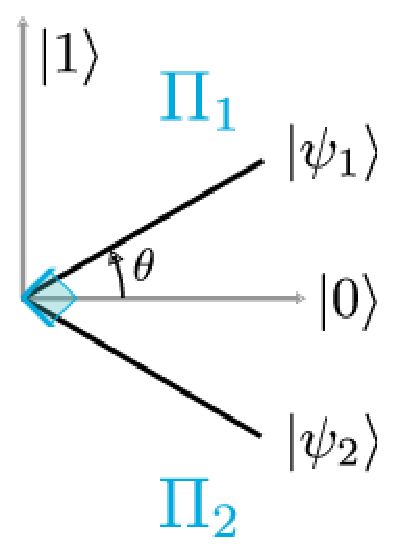
\includegraphics[width=8.5cm,height=8.5cm]{ME}\protect\caption[\hspace{1cm}Min Error]{ The states $\psi_i$ and projectors $\Pi_i = \kb {\phi_i}{\phi_i}$ which minimizes the error rate for detection.
along the states $\left\{ \protect\ket{\psi_{1}},\protect\ket{\psi_{2}}\right\} $
for $\eta_{1}=\eta_{2}=\frac{1}{2}$. }

\par\end{centering}

\label{POVM_ME} 
\end{figure}

We provide a derivation of this result to demonstrate the Neumark formalism.
Since both $\psi_1$ and $\psi_2$ can now evolve to either $0$ or $1$, we must write the unitary equations as
\begin{eqnarray}
U \ke{\psi_1} = \sqrt{p_1} \ke 1 + \sqrt{r_1} \ke 2\\
U \ke{\psi_2} = \sqrt{p_2} \ke 2 + \sqrt{r_2} \ke 1,\label{eq:ME neumark}
\end{eqnarray}
where $p_i$ and $r_i$ are the individual success and error probabilities of the measurement.  Taking the inner product of these 
two equations with themselves we find $p_i + r_i = 1$, and taking the inner product with each other we get the overlap constraint

\begin{equation}
s = \bk{\psi_1}{\psi_2} = \sqrt{p_1 r_2} + \sqrt{ p_2 r_1}, \label{eq:ME constraint}
\end{equation}

We wish to minimize the average error rate

\begin{equation}
P_{E}=\eta_{1}r_{1}+\eta_{2}r_{2},\label{eq:ME}
\end{equation}

subject to the constraint in (\ref{eq:ME constraint}).  We solve this two variable problem using the method of Lagrange multipliers.  
For details on this method see Appendix 2.  The constrained error equation can be written as

\begin{equation}
F(r_1,r_2,\lambda)=\eta_{1}r_{1}+\eta_{2}r_{2}+\lambda\left[s-\sqrt{(1-r_{1})r_{2}}-\sqrt{(1-r_{2})r_{1}}\right].
\end{equation}

Our extrema will be found when all partial derivatives of this equation are zero, therefore

\[
\frac{\partial F_{E}}{\partial r_{1}}=\eta_{1}+\frac{1}{2}\left[\sqrt{\frac{r_{2}}{1-r_{1}}}-\sqrt{\frac{1-r_{2}}{r_{1}}}\right]=0,
\]
and

\[
\frac{\partial F_{E}}{\partial r_{2}}=\eta_{2}+\frac{1}{2}\left[-\sqrt{\frac{r_{1}}{1-r_{2}}}+\sqrt{\frac{1-r_{1}}{r_{2}}}\right]=0.
\]

We notice that these two equations may be re-arranged such that the left hand side is dependent on a single variable:


\begin{equation}
\frac{2\eta_{1}}{\lambda}\sqrt{r_{1}(1-r_{1})}=\sqrt{r_{1}r_{2}}-\sqrt{(1-r_{1})(1-r_{2})},\label{eq:r12}
\end{equation}


\begin{equation}
\frac{2\eta_{2}}{\lambda}\sqrt{r_{2}(1-r_{2})}=\sqrt{r_{1}r_{2}}-\sqrt{(1-r_{1})(1-r_{2})}.\label{eq:r1r2}
\end{equation}


The right hand sides of Eq.(\ref{eq:r12}) and (\ref{eq:r1r2}) can
be set to a constant $\frac{2\eta_{i}}{\lambda}\sqrt{r_{i}(1-r_{i})}\equiv C$,
which can later be determined from the unitarity constraint \ref{eq:ME constraint}, 

\begin{eqnarray}
r_{i} & = & \frac{1}{2}\left(1\pm\sqrt{1-\frac{\lambda^{2}C^{2}}{\eta_{i}^{2}}}\right)=\frac{1}{2}\left(1-\sqrt{1-\frac{\delta^{2}}{\eta_{i}^{2}}}\right),\label{eq:r_i-1}\\
r_{i} & = & \frac{1}{2}\left[1-A_{i}\right],
\end{eqnarray}


where $A_{i}\equiv\sqrt{1-\frac{\delta^{2}}{\eta_{i}^{2}}}$ and $\delta^{2}\equiv\lambda^{2}C^{2}$.
The smaller $r_{i}$ is picked (lower sign in \ref{eq:r_i-1} ) as
this represents error rate, which is to be minimized. Now replace
$r_{i}$ into the constraint (\ref{eq:ME constraint}) and solve for
$\delta$:

\begin{eqnarray*}
s & = & \sqrt{(1-r_{1})r_{2}}+\sqrt{(1-r_{2})r_{1}},\\
2s & = & \sqrt{(1+A_{1})(1-A_{2})}+\sqrt{(1-A_{1})(1+A_{2})},\\
2s^{2} & = & 1-A_{1}A_{2}+\sqrt{(1-A_{1}^{2})(1-A_{2}^{2})},\\
2s^{2} & = & 1-A_{1}A_{2}+\frac{\delta^{2}}{\eta_{1}\eta_{2}},\\
(2s^{2}-1 & -\frac{\delta^{2}}{\eta_{1}\eta_{2}})^{2}= & 1-\frac{\delta^{2}}{\eta_{1}^{2}}-\frac{\delta^{2}}{\eta_{2}^{2}}+\frac{\delta^{4}}{\eta_{1}^{2}\eta_{2}^{2}}.
\end{eqnarray*}


After some tedious but trivial algebra:

\begin{equation}
\delta^{2}=\frac{4s^{2}(1-s^{2})\eta_{1}^{2}\eta_{2}^{2}}{1-4\eta_{1}\eta_{2}s^{2}}.\label{eq:delta}
\end{equation}


Now substitute the value of $\delta$ from (\ref{eq:delta}) into
(\ref{eq:r_i-1}) to get the explicit form of the individual error
rates,

\begin{equation}
r_{i}=\frac{1}{2}\left[1-\frac{1-2\eta_{i}s^{2}}{\sqrt{1-4\eta_{1}\eta_{2}s^{2}}}\right]
\end{equation}


Inserting $r_{1}$ and $r_{2}$ into (\ref{eq:P_E}) Helstrom bound
is retrieved \cite{Helstrom1969}

\begin{eqnarray}
P_{E} & = & \frac{1}{2}\left[1-\frac{\eta_{1}-2\eta_{1}\eta_{2}s^{2}}{\sqrt{1-4\eta_{1}\eta_{2}s^{2}}}-\frac{\eta_{2}-2\eta_{1}\eta_{2}s^{2}}{\sqrt{1-4\eta_{1}\eta_{2}s^{2}}}\right],\nonumber \\
P_{E} & = & \frac{1}{2}\left[1-\sqrt{1-4\eta_{1}\eta_{2}s^{2}}\right].
\end{eqnarray}

%%%%%%%%%%%%%%%%%%%%%%%%%%%%%%%%%%%%%%%%%%%%%%%%
%%%%%%%%%%%%%%%%%%%%%%%%%%%%%%%%%%%%%%%%%%%%%%%%
\section{Unambiguous Discrimination}

It was noticed by *UD CITations** that we may completely eliminate error from the measurement results
by giving up the constraint that our two measurement operators span the whole space, $\Pi_1 + \Pi_2 = I$.  This creates an additional result which 
is not associated with the state being either $\psi_1$ or $\psi_2$ .  It is called the inconclusive or failure outcome $\Pi_0$,
and the new decomposition of the identity reads $\Pi_0+ \Pi_1 + \Pi_2 = I$.  


\begin{eqnarray}
\Pi_{1} & = & \frac{p_{1}}{|\langle\psi_{1}|\psi_{2}^{\perp}\rangle|^{2}}|\psi_{2}^{\perp}\rangle\langle\psi_{2}^{\perp}|,\nonumber \\
\Pi_{2} & = & \frac{p_{2}}{|\langle\psi_{2}|\psi_{1}^{\perp}\rangle|^{2}}|\psi_{1}^{\perp}\rangle\langle\psi_{1}^{\perp}|.\label{eq:Pi1Pi2}
\end{eqnarray}


To determine the failure operator, insert (\ref{eq:Pi1Pi2}) into
(\ref{eq:3povms}): 

\begin{equation}
\Pi_{0}=I-\Pi_{1}-\Pi_{2}=I-\frac{p_{1}}{|\langle\psi_{1}|\psi_{2}^{\perp}\rangle|^{2}}|\psi_{2}^{\perp}\rangle\langle\psi_{2}^{\perp}|-\frac{p_{2}}{|\langle\psi_{2}|\psi_{1}^{\perp}\rangle|^{2}}|\psi_{1}^{\perp}\rangle\langle\psi_{1}^{\perp}|.
\end{equation}

The eigenvalues of $\Pi_{0}$ must be non-negative, giving us the inequality constraint between the individual failure rates as

\begin{equation}
q_{1}q_{2}\geq|\langle\psi_{1}|\psi_{2}\rangle|^{2}.\label{eq:qConstraint}
\end{equation}
 where we used $q_{i}=1-p_{i}.$

Now our value of merit will be the average failure rate $Q = \eta_1 q_1 + \eta_2 q_2$.  Since there is no error the success and failure
add to one: $P_s + Q = 1$.  Hence we wish to minimize the failure rate by taking the equality in Eq. (\ref{eq:qConstraint}), giving us the minimum
failure rate at
\begin{equation}
Q \equiv Q_0 = 2 \sqrt{\eta_1 \eta_2}|\langle\psi_{1}|\psi_{2}\rangle|. \label{Q0}
\end{equation}

This solution is valid for $q_{i}\leq1.$  Outside of this bound we ignore the state with the high rate of failure by removing that detector and
reducing our measurement strategy back to projective measurements.  We project onto the more likely state.  Therefore the total UD solution is
\begin{equation}
Q_{{\rm c}}=\left\{ \begin{array}{l}
\eta_{1}+\eta_{2}\cos^{2}\theta,\mbox{if \ensuremath{{\displaystyle \eta_{1}<\frac{\cos^{2}\theta}{1+\cos^{2}\theta}\equiv\eta_{1}^{(l)}}},}\\[0.7em]
\eta_{2}+\eta_{1}\cos^{2}\theta,\mbox{if \ensuremath{\eta_{1}>{\displaystyle \frac{1}{1+\cos^{2}\theta}\equiv\eta_{1}^{(r)}}},}\\[0.7em]
2\sqrt{\eta_{1}\eta_{2}}\cos\theta\equiv Q_{0},\mbox{if \ensuremath{\eta_{1}^{(l)}\le\eta_{1}\le\eta_{1}^{(r)}}}\ ,
\end{array}\right.\label{Qmax}
\end{equation}



%%%%%%%%%%%%%%%%%%%%%%%%%%%%%%%%%%%%%%%%%%%%%%%%
%%%%%%%%%%%%%%%%%%%%%%%%%%%%%%%%%%%%%%%%%%%%%%%%
\section{Interpolative Discrimination}
\subsection{Operator Transformation}


%[floatfix]
\begin{figure}[ht!]
\centering{ 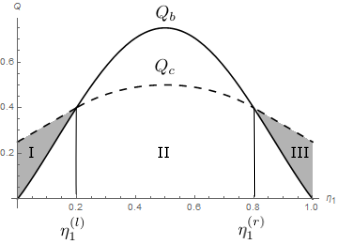
\includegraphics[height=4.5cm]{Fig1.png}}
\protect\caption[\hspace{1cm}$Q_{{\rm c}}$ and $Q_{{\rm b}}$ vs.~$\eta_{1}$]{ $Q_{{\rm c}}$ (dashed line, Eq. (\ref{Qmax})) and $Q_{{\rm b}}$
(solid line, Eq. (\ref{Qb})) vs.~$\eta_{1}$ for $\theta=\pi/3$.
Measurements can be optimized in the area under the dashed line, $Q_{c}$.
Measurements in the area above $Q_{c}$ are suboptimal. In the shaded
areas between $Q_{c}$ and $Q_{b}$ (regions I, left, and III, right)
the optimal FRIO measurement is a projective measurement, in the unshaded
area below $Q_{c}$ (region II) the optimal measurement is a POVM.}
\label{Fig1} 
\end{figure}


We review the original problem in a single two-dimensional Hilbert space, and the solution that  involves a transformation that eliminates the failure operator from the discrimination problem.  We are given two pure states $\rho_1= \ke \psi_1 \br {\psi_1}$ and $\rho_2 = \ke \psi_2 \br{\psi_2}$ with a-priori probabilities $\eta_1$ and $\eta_2$ respectively.  These two probabilities add to one:  $\eta_1 +\eta_2 = 1$. We wish to optimize the success rate  $P_s = \eta_1tr[\Pi_1 \rho_1] + \eta_2 tr[\Pi_2 \rho_2]$ for a fixed failure rate $Q = tr[\Pi_0(\eta_1 \rho_1 + \eta_2 \rho_2)]$ where the measurement operators are the $\Pi_i$ that span the Hilbert space: $\Pi_1 + \Pi_2 + \Pi_0 = I$.  The transformation we implement is
 \begin{equation}
\Omega ^{-1/2}[\Pi_1 + \Pi_2] \Omega^{-1/2} = I,
\end{equation}
where $\Omega = I - \Pi_0$.

Calling the transformed operators $\widetilde \Pi_i$ for $i= 1,2$, we can find the corresponding transformed density matrices $\widetilde \rho_i$ and a-priori probabilities $
\widetilde \eta_i$ to make this a new ME problem that can be readily solved. The minimized error probability as a function of the failure rate is
\begin{equation} P_e = \frac{1}{2} (1 - Q -\sqrt{(1-Q)^2 - (Q-Q_0)^2})\end{equation}
for $Q \leq Q_0 = 2 \sqrt{\eta_1\eta_2} \cos \theta$ where $Q_0$ is the maximum failure rate allowed in the optimization scheme and it corresponds to the best measurement in the UD case.  We will provide an in-depth description of this solution as it pertains to our problem in the next section.



%%%%%%%%%%%%%%%%%%%%%%%%%%%%%%%%%%%%%%%%%%%%%%%%
%%%%%%%%%%%%%%%%%%%%%%%%%%%%%%%%%%%%%%%%%%%%%%%%
\subsection{Analytical Solution of Interpolation}

In this section we solve the interpolation with FRIO in two different
ways. In the first method, through a parametrization, the problem
is converted into a minimum error whose solution is well known. Then
there is one last optimization with respect to a FRIO. This method
generates the same solution as in Bagan $et$ $al$ in a few lines.
However to obtain an experimental realization we give an alternative
solution using Neumark's theorem. It is a generalized measurement
procedure in which the system is embedded in a larger Hilbert space
with extra degrees of freedom. A unitary transformation entangles
the system with the extra degree of freedom known as ancilla. After
this interaction has taken place, projective von Neumann measurements
are carried out on the ancilla. Our input states are qubits, which
can be expressed in general as unit length vectors in the two dimensional
basis spanned by $|1\rangle$ and $|2\rangle$. In the output of the
transformation, we associate the basis state $|1\rangle$ with $|\psi_{1}\rangle$,
$|2\rangle$ with $|\psi_{2}\rangle$, and $|0\rangle$ gives no information
about the system. The unitary transformation should do the following:

\begin{align}
U|\psi_{1}\rangle_{s}|0\rangle_{a} & =\sqrt{p_{1}}|1\rangle_{s}\ket 1_{a}+\sqrt{r_{1}}|2\rangle_{s}\ket 2_{a}+\sqrt{q_{1}}|0\rangle_{s}\ket 0_{a},\nonumber \\
U|\psi_{2}\rangle_{s}|0\rangle_{a} & =\sqrt{r_{2}}|1\rangle_{s}\ket 1_{a}+\sqrt{p_{2}}|2\rangle_{s}\ket 2_{a}+\sqrt{q_{2}}|0\rangle_{s}\ket 0_{a},\label{eq:frio constraint}
\end{align}
where: $p_{i}$ is the probability that state $i\thinspace(i=1,2)$
is correctly identified, $r_{i}$ is the probability that the detector
mistakenly identifies state $i$ for $j$, and $q_{i}$ is the failure
probability, the detector fails to identify the state at all. A click
in the ancilla $|0\rangle_{a}$ means the results are inconclusive
and we learn nothing from the measurement. From the unitarity conditions
we obtain the normalized probabilities $p_{i}+r_{i}+q_{i}=1$.

We wish to maximize the probability of success, $P_{s}=\eta_{1}p_{1}+\eta_{2}p_{2}$,
and minimize the error rate, $P_{e}=\eta_{1}r_{1}+\eta_{2}r_{2}$,
for a fixed failure rate $Q=\eta_{1}q_{1}+\eta_{2}q_{2}.$ Clearly
$P_{s}+P_{e}+Q=1$.

The inner product of the two equations in (\ref{eq:frio constraint})
gives the overlap of the input states in terms of $r_{i},\thinspace p_{i}$
and $q_{i}$, 
\begin{equation}
s=\sqrt{p_{1}r_{2}}+\sqrt{p_{2}r_{1}}+\sqrt{q_{1}q_{2}},\label{eq:general constraint}
\end{equation}
where $s\equiv\langle\psi_{1}|\psi_{2}\rangle$. This is a constraint
on the optimization of ME with a FRIO. First we show the solution
for the case when the input states are prepared with equal priors
for which the problem is fully solved from the constraint. It was
initially solved by Chefles and Barnett using a different approach
\cite{Chefles1998}. Then we solve the general case for different
priors and reproduce the results of Bagan $et\thinspace al.$ with
two different methods. 

%%%%%%%%%%%%%%%%%%%%%%%%%%%%%%%%%%%%%%%%%%%%%%%%
%%%%%%%%%%%%%%%%%%%%%%%%%%%%%%%%%%%%%%%%%%%%%%%%
\subsection{Equal priors. }

Let us first present the solution where the incoming states are given
with equal a-priori probabilities, $\eta_{1}=\eta_{2}=\frac{1}{2}$.
This implies equal error, success and failure rates: $r_{1}=r_{2}$
, $p_{1}=p_{2}$ and $q_{1}=q_{2}$. Thus the total error and failure
rates reduce to: $P_{E}=\eta_{1}r_{1}+\eta_{2}r_{2}=r$ and $Q=\eta_{1}q_{1}+\eta_{2}q_{2}=q.$ 

We can immediately solve the constraint in Equation (\ref{eq:general constraint})
by replacing $p=1-r-Q$, solving the quadratic equation for the error
rate in terms of the failure rate and overlap $s$, which is also
the overall failure rate in the IDP limit for the equal priors: $Q_{o}\equiv2\sqrt{\eta_{1}\eta_{2}}s=s$, 

\begin{eqnarray}
s & = & \sqrt{pr}+\sqrt{pr}+Q,\nonumber \\
Q_{o} & = & 2\sqrt{r(1-r-Q)}+Q,\nonumber \\
(Q_{o}-Q)^{2} & = & 4r(1-r-Q),\nonumber \\
\frac{1}{4}(Q_{o}-Q)^{2} & = & r(1-Q)-r^{2},\nonumber \\
0 & = & r^{2}-(1-Q)r+\frac{1}{4}(Q_{o}-Q)^{2}.\label{eq:quadratic IM}
\end{eqnarray}
Solving the quadratic equation and taking the smaller root, $i.e$
the smaller error rate:

\begin{eqnarray}
r=P_{E}=\frac{1}{2}[(1-Q)-\sqrt{(1-Q)^{2}-(Q_{o}-Q)^{2}}],\\
p=P_{S}=\frac{1}{2}[(1-Q)+\sqrt{(1-Q)^{2}-(Q_{o}-Q)^{2}}].
\end{eqnarray}


The equal priors case requires no further optimization. Simply solving
the quadratic equation in (\ref{eq:quadratic IM}) derived from the
constraint the optimal solution is carried out. By varying the failure
rate $Q$ from zero to $Q_{o}$ we recover the Helstrom and IDP bounds.
In the Helstrom bound \cite{Helstrom1969} one is not allowed to have
inconclusive results, hence setting failure rate to zero, $Q=0$ results
in 

\begin{equation}
P_{E}=\frac{1}{2}[1-\sqrt{1-Q_{o}^{2}}]
\end{equation}


In the IDP limit \cite{Ivanovic1987,Dieks1988,Peres1988} where one
is not allowed to make an error $r=0,$ while allowing for inconclusive
outcomes:

\begin{eqnarray*}
0 & = & \frac{1}{2}[(1-Q)-\sqrt{(1-Q)^{2}-(Q_{o}-Q)^{2}}],\\
Q & = & Q_{o},
\end{eqnarray*}
where $Q_{o}$ in the overlap of the input states for equal priors
$Q_{o}=s.$ 

%%%%%%%%%%%%%%%%%%%%%%%%%%%%%%%%%%%%%%%%%%%%%%%%
%%%%%%%%%%%%%%%%%%%%%%%%%%%%%%%%%%%%%%%%%%%%%%%%
\subsection{Arbitrary priors }

Because of the recent interest in this problem, we feel it is beneficial
to show two new and different approaches to its solution. The first
is more conceptual: a renormalization inspired by E. Bagan et al.
\cite{Bagan2012} allows us to rewrite the problem as a ME problem
with an implicit dependence on the last free parameter, the failure
rate of one state with relation to the other. This greatly simplifies
the problem as the solution to the first part is well known and the
second is a straight-forward derivative. The second solution employs
a Lagrange multiplier method that is algebraically difficult but useful
in its explicit results of individual error rates. This in turn is
useful in designing an implementation scheme where the reflective
and transmittance coefficients are expressed in terms of individual
error and success rate. 

%%%%%%%%%%%%%%%%%%%%%%%%%%%%%%%%%%%%%%%%%%%%%%%%
%%%%%%%%%%%%%%%%%%%%%%%%%%%%%%%%%%%%%%%%%%%%%%%%
\subsection{Transformation of the problem into the Helstrom form}

Through a renormalization our problem is converted into the well known
Helstrom form the solution of which is well known. First we define
the useful quantity $\omega\equiv s-\sqrt{q_{1}q_{2}}$ which will
serve as normalized overlap and the unitarity constraint from Eq.(\ref{eq:general constraint})
reduces to: 
\begin{equation}
\omega=\sqrt{p_{1}r_{2}}+\sqrt{p_{2}r_{1}}.
\end{equation}


Next we renormalize all probabilities in the problem: 
\begin{align}
 & \tilde{p}_{i}=\frac{p_{i}}{\alpha_{i}},\nonumber \\
 & \tilde{r_{i}}=\frac{r_{i}}{\alpha_{i}},\nonumber \\
 & \tilde{\omega}=\frac{\omega}{\alpha_{1}\alpha_{2}},\\
\nonumber 
\end{align}
where $\alpha_{i}=1-q_{i}$. Now the probabilities are normalized
$\widetilde{r}_{i}+\tilde{p}_{i}=1$, and the new normalized overlap
is in terms of $\tilde{r_{i}}$ and $\tilde{p}_{i},$

\begin{equation}
\tilde{\omega}=\sqrt{\tilde{p}_{1}\tilde{r}_{2}}+\sqrt{\tilde{p_{2}}\tilde{r}_{1}}
\end{equation}


Using the above transformation of $r_{i}$ the error rate can be expressed
as: 
\begin{equation}
\tilde{P}_{E}=\tilde{\eta}_{1}\tilde{r}_{1}+\tilde{\eta}_{2}\tilde{r}_{2},
\end{equation}
where $\tilde{P}_{E}=\frac{P_{E}}{\eta_{1}\alpha_{1}+\eta_{2}\alpha_{2}}=\frac{P_{E}}{1-Q},\tilde{\eta}_{i}=\frac{\eta_{i}\alpha_{i}}{\eta_{1}\alpha_{1}+\eta_{2}\alpha_{2}}=\frac{\eta_{i}\alpha_{i}}{1-Q}$
and $\tilde{\eta}_{1}+\tilde{\eta}_{2}=1$.

We have transformed the problem into a discrimination between two
pure states with overlap $\tilde{\omega}$ and no explicit failure
rate. Hence we can simply write down the expression for the minimum
error solution of two pure states (the Helstrom bound), and then replace
the normalized quantities with the original expressions: 
\begin{align}
\tilde{P}_{E} & =\frac{1}{2}[1-\sqrt{1-4\tilde{\eta}_{1}\tilde{\eta}_{2}\tilde{\omega}^{2}}],\nonumber \\
P_{E} & =\frac{1}{2}[(1-Q)-\sqrt{(1-Q)^{2}-4\eta_{1}\eta_{2}(s-\sqrt{q_{1}q_{2}})^{2}}].\label{eq:optimize P_e}
\end{align}


There is now one last optimization. Given a fixed rate of the average
of inconclusive outcomes, $Q,$ what are the individual failure rates
$q_{i}.$ To minimize Eq. (\ref{eq:optimize P_e}) we maximize the
square root term $\sqrt{(1-Q)^{2}-4\eta_{1}\eta_{2}(s-\sqrt{q_{1}q_{2}})^{2}},$
which in turn means to minimize $(s-\sqrt{q_{1}q_{2}})^{2}=(s^{2}+q_{1}q_{2}-2s\sqrt{q_{1}q_{2}}).$
The overlap term $s^{2}$ is fixed and we are left with $q_{1}q_{2}-2s\sqrt{q_{1}q_{2}.}$
Only one of the $q_{i}'s$ is an independent variable as we fix the
overall failure rate $Q=\eta_{1}q_{1}+\eta_{2}q_{2},$ 

\begin{eqnarray*}
\Theta & = & q_{1}q_{2}-2s\sqrt{q_{1}q_{2}.}\\
\Theta & = & \frac{q_{1}(Q_{0}-\eta_{1}q_{1}^{2})}{\eta_{2}}-2s\sqrt{\frac{q_{1}(Q_{0}-\eta_{1}q_{1}^{2})}{\eta_{2}}}\\
\Theta & = & \frac{\eta_{1}q_{1}Q_{0}-\eta_{1}^{2}q_{1}^{2}}{\eta_{1}\eta_{2}}-2s\sqrt{\frac{\eta_{1}q_{1}Q_{0}-\eta_{1}^{2}q_{1}^{2}}{\eta_{1}\eta_{2}}}\\
\Theta & = & \frac{\tilde{q}_{1}Q_{0}-\tilde{q}_{1}^{2}}{\eta_{1}\eta_{2}}-2s\sqrt{\frac{\tilde{q}_{1}Q_{0}-\tilde{q}_{1}^{2})}{\eta_{1}\eta_{2}}}
\end{eqnarray*}


where $\eta_{1}q_{1}=\tilde{q}.$ Let's optimize with respect to $\tilde{q}_{1}.$

\begin{equation}
0=\frac{\partial\Theta}{\partial\tilde{q}_{1}}=\frac{Q_{0}-2\tilde{q}_{1}}{\eta_{1}\eta_{2}}-2s\sqrt{\frac{Q_{0}-2\tilde{q}_{1}}{\eta_{1}\eta_{2}}}
\end{equation}


this leads to the optimality condition $Q_{0}=2\tilde{q}_{1}=2\eta_{1}q_{1}=2\eta_{2}q_{2},$
giving the minimal error rate in discriminating two pure states with
a fixed rate of failure as 
\begin{equation}
P_{E}=\frac{1}{2}[(1-Q)-\sqrt{(1-Q)^{2}-(Q_{o}-Q)^{2}}].\label{eq:frio}
\end{equation}
Here $Q_{o}=2\sqrt{\eta_{1}\eta_{2}}s$ is the failure rate in the
optimal unambiguous state discrimination, which our expression reaches
when we set $P_{E}=0$. On the other hand when the failure rate is
zero we can recover the Helstrom bound for two pure states $P_{E}=\frac{1}{2}[1-\sqrt{1-4\eta_{1}\eta_{2}s^{2}}].$ 


%%%%%%%%%%%%%%%%%%%%%%%%%%%%%%%%%%%%%%%%%%%%%%%%
%%%%%%%%%%%%%%%%%%%%%%%%%%%%%%%%%%%%%%%%%%%%%%%%
\subsection{Lagrange Multipliers Method}

While the above method gives a closed form solution of the average
error rate in terms of a FRIO it does not produce individual error
or success rates, i.e the error rates of mistaking state $|\psi_{i}\rangle$
for state $|\psi_{j}\rangle$ , which are needed for the implementation
in calculating the transmittance and reflection coefficients of the
beam splitters. To obtain these expressions we show another solution
to the interpolation using the Lagrange multipliers method with the
constraint in Eq. (\ref{eq:general constraint}). 

We want to minimize the average error rate $P_{E}=\eta_{1}r_{1}+\eta_{2}r_{2}$
subject to the constraint $s=\sqrt{(1-r_{1}-q_{1})r_{2}}+\sqrt{(1-r_{2}-q_{2})r_{1}}+\sqrt{q_{1}q_{2}},$
setting up the function with one Lagrange multiplier $\lambda:$ 

\begin{equation}
F=\eta_{1}r_{1}+\eta_{2}r_{2}+\lambda(s-\sqrt{(1-r_{1}-q_{1})r_{2}}-\sqrt{(1-r_{2}-q_{2})r_{1}}-\sqrt{q_{1}q_{2}}).
\end{equation}


Setting the derivative $dF_{(r_{1},r_{2},\lambda)}/dr_{i}$ to zero
then solving for $r_{i}(\lambda)$, we exploit the symmetry in the
resulting equations to solve for the individual error rates $r_{i}$
as a function of the failure rates $q_{i}$. Subsequent substitution
into the constraint gives us the optimal value of $\lambda$. Then
we can obtain the total minimum error by replacing the expressions
of $r_{i}$ into $P_{e}$ and minimizing $P_{e}$ under the additional
constraint that $\eta_{1}q_{1}+\eta_{2}q_{2}=Q$. This gives us the
optimal relationship between failure rates as $\eta_{1}q_{1}=\eta_{2}q_{2}$
and the total optimal error rate as $Q=2\eta_{1}q_{1}=2\eta_{2}q_{2}.$

Setting $dF/dr_{1}=0$ and re-arranging we get: 

\[
(2\eta_{1}/\lambda)\sqrt{(1-q_{1}-r_{1})r_{1}}=\sqrt{(1-q_{2}-r_{2})(1-q_{1}-r_{1})}-\sqrt{r_{1}r_{2}}.
\]


Similarly $dF/dr_{2}=0$ gives 
\begin{equation}
(2\eta_{2}/\lambda)\sqrt{(1-q_{2}-r_{2})r_{2}}=\sqrt{(1-q_{2}-r_{2})(1-q_{1}-r_{1})}-\sqrt{r_{1}r_{2}}.
\end{equation}


This step is algebraically challenging and requires the insight that
the resulting equations can each be separated into two expressions,
left hand side depending on only $r_{1}$ or $r_{2}$ and the right
hand sides are equivalent. Because both equations have the same multivariable
expression, we can set the left hand sides equal to a constant, $C,$
which is yet to be determined. 
\begin{equation}
(2\eta_{1}/\lambda)\sqrt{(1-q_{1}-r_{1})r_{1}}=(2\eta_{2}/\lambda)\sqrt{(1-q_{2}-r_{2})r_{2}}\equiv C.
\end{equation}
This greatly simplifies the problem, turning it into a quadratic equation. 

\begin{equation}
(2\eta_{i}/\lambda)\sqrt{(1-q_{i}-r_{i})r_{i}}=C.\label{eq:C}
\end{equation}
Let $\alpha_{i}\equiv1-q_{i}$ 
\begin{eqnarray*}
\sqrt{(\alpha_{1}-r_{i})r_{i}} & = & (\lambda C)/(2\eta_{i}),\\
r_{i}^{2}-\alpha_{i}r_{i}+\lambda^{2}C^{2}/4\eta_{i}^{2} & = & 0,\\
r_{i}(\pm) & = & 1/2\left(\alpha_{i}\pm\sqrt{\alpha_{i}^{2}-\frac{\lambda^{2}C^{2}}{\eta_{i}^{2}}}\right).
\end{eqnarray*}
$r_{i}$ is the error rate which we want to be minimized, thus we
take the smaller root $r_{i}(-).$ 

\begin{eqnarray}
r_{1} & = & 1/2\left(\alpha_{1}-\sqrt{\alpha_{1}^{2}-\frac{\delta}{\eta_{1}^{2}}}\right)=1/2\left(\alpha_{1}-A_{1}\right),\label{eq:r1(lambda)}\\
r_{2} & = & 1/2\left(\alpha_{2}-\sqrt{\alpha_{2}^{2}-\frac{\delta}{\eta_{2}^{2}}}\right)=1/2\left(\alpha_{2}-A_{2}\right),\label{eq:r2(lambda)}
\end{eqnarray}
 where $\delta\equiv\lambda^{2}C^{2}$ and $A_{i}\equiv\sqrt{\alpha_{i}^{2}-(\frac{\lambda^{2}C^{2}}{\eta_{i}^{2}})}.$ 

Insert the expression of $r_{i}$ from (\ref{eq:r1(lambda)}) and
(\ref{eq:r2(lambda)}) into the constraint from (\ref{eq:general constraint}).
First let us rewrite the constraint so it simplifies the algebra later: 

\[
\omega=(1-r_{1}-q_{1})r_{2}+(1-r_{2}-q_{2})r_{1}+\sqrt{(1-r_{1}-q_{1})(1-r_{2}-q_{2})r_{1}r_{2}}
\]


where $\omega\equiv(s-\sqrt{q_{1}q_{2}})^{2}$. We use the definition
in (\ref{eq:C}) to reduce the square root term

$\sqrt{(1-r_{1}-q_{1})(1-r_{2}-q_{2})r_{1}r_{2}}=\frac{\lambda^{2}C^{2}}{4\eta_{1}\eta_{2}},$
giving

\[
(s-\sqrt{q_{1}q_{2}})^{2}=(1-r_{1}-q_{1})r_{2}+(1-r_{2}-q_{2})r_{1}+\frac{\lambda^{2}C^{2}}{4\eta_{1}\eta_{2}}.
\]
Using $\alpha_{i}=1-q_{i},$ the above expression becomes:

\begin{eqnarray*}
\omega & = & (\alpha_{1}-q_{1})r_{2}+(\alpha_{2}-q_{2})r_{1}+\frac{\delta}{4\eta_{1}\eta_{2}}\\
 & = & \alpha_{1}r_{2}-\alpha_{2}r_{1}-2r_{1}r_{2}+\frac{\delta}{4\eta_{1}\eta_{2}}\\
 & = & \frac{\alpha_{1}}{2}\left(\alpha_{2}-A_{2}\right)+\frac{\alpha_{2}}{2}\left(\alpha_{1}-A_{1}\right)-\frac{1}{2}\left(\alpha_{1}-A_{1}\right)\left(\alpha_{2}-A_{2}\right)+\frac{\delta}{4\eta_{1}\eta_{2}}\\
 & = & \alpha_{1}\alpha_{2}-A_{1}A_{2}+\frac{\delta}{4\eta_{1}\eta_{2}}.
\end{eqnarray*}
Replacing $A_{i}$ by their respective value

\begin{eqnarray*}
\omega & = & \frac{1}{2}\left[\alpha_{1}\alpha_{2}-\sqrt{\alpha_{1}^{2}-\frac{\delta}{\eta_{1}^{2}}}\sqrt{\alpha_{2}^{2}-\frac{\delta}{\eta_{2}^{2}}}+\delta/\eta_{1}\eta_{2}\right],\\
\sqrt{\alpha_{1}^{2}-\frac{\delta}{\eta_{1}^{2}}}\sqrt{\alpha_{2}^{2}-\frac{\delta}{\eta_{2}^{2}}} & = & \alpha_{1}\alpha_{2}+\delta/\eta_{1}\eta_{2}-2\omega.
\end{eqnarray*}
Squaring both sides, using $\frac{\alpha_{1}}{\eta_{2}}+\frac{\alpha_{2}}{\eta_{1}}=\frac{\alpha_{1}\eta_{1}+\alpha_{2}\eta_{2}}{\eta_{1}\eta_{2}}=\frac{\eta_{1}(1-q_{1})+\eta_{2}(1-q_{2})}{\eta_{1}\eta_{2}}=\frac{1-Q}{\eta_{1}\eta_{2}}$
and after some trivial algebra we get:

\begin{eqnarray}
\delta\left[\frac{4\omega}{\eta_{1}\eta_{2}}-\left(\frac{\alpha_{1}}{\eta_{2}}+\frac{\alpha_{2}}{\eta_{1}}\right)\right] & = & 4\omega^{2}-4\omega\alpha_{1}\alpha_{2},\nonumber \\
\delta\left[\frac{4\omega}{\eta_{1}\eta_{2}}-\frac{(1-Q)^{2}}{\eta_{1}^{2}\eta_{2}^{2}}\right] & = & 4\omega^{2}-4\omega\alpha_{1}\alpha_{2},\nonumber \\
\delta & = & \frac{\left(\omega^{2}-\omega\alpha_{1}\alpha_{2}\right)4\eta_{1}^{2}\eta_{2}^{2}}{4\omega\eta_{1}\eta_{2}-(1-Q)^{2}},
\end{eqnarray}
Now substitute $\delta$ into $r_{1}$ in (\ref{eq:r1(lambda)}) 
\begin{eqnarray}
r_{1} & = & \frac{1}{2}\left(\alpha_{1}-\sqrt{\alpha_{1}^{2}-\frac{\lambda^{2}C^{2}}{\eta_{1}^{2}}}\right)\nonumber \\
 & = & \frac{1}{2}\left(\alpha_{1}-\sqrt{\alpha_{1}^{2}-\frac{1}{\eta_{1}^{2}}\frac{(\omega^{2}-\omega\alpha_{1}\alpha_{2})4\eta_{1}^{2}\eta_{2}^{2}}{4\omega\eta_{1}\eta_{2}-(1-Q)^{2}}}\right)\nonumber \\
 & = & \frac{1}{2}\left(\alpha_{1}-\sqrt{\frac{\alpha_{1}^{2}[4\omega\eta_{1}\eta_{2}-(1-Q)^{2}]-4\eta[\omega^{2}-\omega\alpha_{1}\alpha_{2}]}{4\omega\eta_{1}\eta_{2}-(1-Q)^{2}}}\right).
\end{eqnarray}


The numerator can be greatly simplified:

$\alpha_{1}^{2}[4\omega\eta_{1}\eta_{2}-(1-Q)^{2}]-4\eta_{2}^{2}[\omega^{2}-\omega\alpha_{1}\alpha_{2}]=-\alpha_{1}^{2}(1-Q)^{2}-4\eta_{2}^{2}\omega^{2}+4\omega\eta_{2}\alpha_{1}[\eta_{1}\alpha_{1}+\eta_{2}\alpha_{2}]$

$=-[\alpha_{1}(1-Q)-2\eta_{2}\omega]^{2}=-[(1-q_{1})(1-Q)-2\eta_{2}(s-\sqrt{q_{1}q_{2}})^{2}]^{2}.$

The calculation for $r_{2}$ goes along the same line. Expression
for $r_{1}$ and $r_{2}$ become:

\begin{eqnarray}
r_{1} & = & \frac{1}{2}\left[\left(1-q_{1}\right)-\frac{\left(1-q_{1}\right)\left(1-Q\right)-2\eta_{2}\left(s-\sqrt{q_{1}q_{2}}\right)^{2}}{\sqrt{(\left(1-Q\right))^{2}-4\eta_{1}\eta_{2}\left(s-\sqrt{q_{1}q_{2}}\right)^{2}}}\right],\\
r_{2} & = & \frac{1}{2}\left[\left(1-q_{2}\right)-\frac{\left(1-q_{2}\right)\left(1-Q\right)-2\eta_{1}\left(s-\sqrt{q_{1}q_{2}}\right)^{2}}{\sqrt{\left(1-Q\right)^{2}-4\eta_{1}\eta_{2}\left(s-\sqrt{q_{1}q_{2}}\right)^{2}}}\right].
\end{eqnarray}
Finally $r_{1}$ and $r_{2}$ can be substituted into the overall
average error rate $P_{E}=\eta_{1}r_{1}+\eta_{2}r_{2}:$ 

\begin{eqnarray}
P_{E} & = & \frac{1}{2}\left[1-\left(\eta_{1}q_{1}+\eta_{2}q_{2}\right)-\frac{\left(1-Q\right)\left(\eta_{1}+\eta_{2}\right)-\left(\eta_{1}q_{1}+\eta_{2}q_{2}\right)-4\eta_{1}\eta_{2}\left(s-\sqrt{q_{1}q_{2}}\right)^{2}}{\sqrt{\left(1-Q\right)^{2}-4\eta_{1}\eta_{2}\left(s-\sqrt{q_{1}q_{2}}\right)^{2}}}\right]\nonumber \\
 & = & \frac{1}{2}\left[(1-Q)-\frac{\left(1-Q\right)^{2}-4\eta_{1}\eta_{2}\left(s-\sqrt{q_{1}q_{2}}\right)^{2}}{\sqrt{\left(1-Q\right)^{2}-4\eta_{1}\eta_{2}\left(s-\sqrt{q_{1}q_{2}}\right)^{2}}}\right]\nonumber \\
 & = & \frac{1}{2}\left[(1-Q)-\sqrt{\left(1-Q\right)^{2}-4\eta_{1}\eta_{2}\left(s-\sqrt{q_{1}q_{2}}\right)^{2}}\right]\label{eq:P_E(q1,q2)}
\end{eqnarray}


It has been showed in previous sections that (\ref{eq:P_E(q1,q2)})
is optimized for a fixed value of failure rate when $\eta_{1}q_{1}=\eta_{2}q_{2}.$
Eq (\ref{eq:P_E(q1,q2)}) then reduces to the now well know FRIO form:

\begin{equation}
P_{E}=\frac{1}{2}\left[(1-Q)-\sqrt{(1-Q)^{2}-(Q-Q_{0})^{2}}\right].
\end{equation}


The individual error and success rates can now be expressed explicitly
in terms of $\eta_{i},$ $Q_{o}$ and most importantly the fixed failure
rate $Q$ as: 
\begin{align}
r_{i} & =\frac{1}{2}\left[\left(1-\frac{Q}{2\eta_{i}}\right)-\frac{\left(1-\frac{Q}{2\eta_{i}}\right)\left(1-Q\right)-\frac{1}{2\eta_{i}}(Q_{o}-Q)^{2}}{\sqrt{(1-Q)^{2}-(Q-Q_{o})^{2}}}\right],\label{eq:r_i}\\
p_{i} & =\frac{1}{2}\left[\left(1-\frac{Q}{2\eta_{i}}\right)+\frac{\left(1-\frac{Q}{2\eta_{i}}\right)\left(1-Q\right)-\frac{1}{2\eta_{i}}(Q_{o}-Q)^{2}}{\sqrt{(1-Q)^{2}-(Q-Q_{o})^{2}}}\right].\label{eq:p_i}
\end{align}

%%%%%%%%%%%%%%%%%%%%%%%%%%%%%%%%%%%%%%%%%%%%%%%%
%%%%%%%%%%%%%%%%%%%%%%%%%%%%%%%%%%%%%%%%%%%%%%%%
%%%%%%%%%%%%%%%%%%%%%%%%%%%%%%%%%%%%%%%%%%%%%%%%
%%%%%%%%%%%%%%%%%%%%%%%%%%%%%%%%%%%%%%%%%%%%%%%%


\chapter{Discrimination of Mixed States}
\section{Minimum Error Discrimination}


%%%%%%%%%%%%%%%%%%%%%%%%%%%%%%%%%%%%%%%%%%%%%%%%
%%%%%%%%%%%%%%%%%%%%%%%%%%%%%%%%%%%%%%%%%%%%%%%%
\subsection{Minimum Error: Two mixed states via POVM }

Given an ensemble of two mixed states $\{\rho_{1},\rho_{2}\}$ prepared
with different a priori probabilities $\{\eta_{1},\eta_{2}\}$ the
task is to minimize the rate for which the detectors misidentify a
state. The minimum error problem for two pure or mixed states was
first solved by Helstrom \cite{Helstrom1969}. We show an alternative
derivation to ME of two pure states developed by Herzog \cite{Herzog2004}
and Fuchs \cite{Fuchs1996}. When the detector $\Pi_{i}$ clicks for
state $\rho_{j}$ it is an error, $r_{i}=Tr(\rho_{j}\Pi_{i})$, a
clink for state $\rho_{i}$ is success $p_{i}=Tr(\rho_{i}\Pi_{i})$.
Thus for two states we want to minimize the following expression. 

\begin{equation}
P_{E}=\eta_{1}Tr(\rho_{1}\Pi_{2})+\eta_{2}Tr(\rho_{2}\Pi_{1}).\label{eq:P_E}
\end{equation}


Using the relation $\eta_{1}+\eta_{2}=1$ and $\Pi_{1}+\Pi_{2}=I$,
Equation (\ref{eq:P_E}) can be rewritten as:

\begin{eqnarray*}
P_{E} & = & \eta_{1}Tr(\rho_{1}(I-\Pi_{1}))+\eta_{2}Tr(\rho_{2}\Pi_{1}),\\
 & = & \eta_{1}+Tr[(\eta_{2}\rho_{2}-\eta_{1}\rho_{1})\Pi_{1},\\
 & = & \eta_{2}-Tr[(\eta_{2}\rho_{2}-\eta_{1}\rho_{1})\Pi_{2}.
\end{eqnarray*}


Let $\Lambda=\eta_{2}\rho_{2}-\eta_{1}\rho_{1}$
\begin{equation}
P_{E}=\eta_{1}+Tr(\Lambda\Pi_{1})=\eta_{2}-Tr(\Lambda\Pi_{2}).
\end{equation}


To minimize $P_{E},$ $\Pi_{1}$ should project onto the eigenvectors
of the negative eigenvalues of $\Lambda,$ on the other hand $\Pi_{2}$
should project onto the positive eigenvectors. Let us write $\Lambda$
into its spectral decomposition. 

\begin{equation}
\Lambda=\eta_{2}\rho_{2}-\eta_{1}\rho_{1}=\sum_{i=1}^{d}\lambda_{i}|\lambda_{i}\rangle\langle\lambda_{i}|.
\end{equation}


To implement the projection of the POVM operators onto the positive
(or negative) eigenvectors the eigenvalues $\lambda_{i}$ can be split
into three categories without any loss of generality: negative, positive
and zero:

\begin{eqnarray}
\lambda_{i} & < & 0\text{ for }1\leq i<i_{o},\nonumber \\
\lambda_{i} & > & 0\text{ for \ensuremath{i_{o}\leq i<d}},\nonumber \\
\lambda_{i} & = & 0\text{ for \ensuremath{d\leq i<d_{s}}. }
\end{eqnarray}


Then from the spectral decomposition we can rewrite $(2.2.6)$ in
terms of the optimal POVM. 

\begin{equation}
P_{E}=\eta_{1}+\sum_{i=1}^{i_{o}-1}\lambda_{i}\langle\lambda_{i}|\Pi_{1}|\lambda_{i}\rangle=\eta_{2}-\sum_{i=i_{o}}^{d_{s}}\lambda_{i}\langle\lambda_{i}|\Pi_{2}|\lambda_{i}\rangle,
\end{equation}
where $\Pi_{1}=\sum_{i=1}^{i_{o}-1}\lambda_{i}|\lambda_{i}\rangle\langle\lambda_{i}|$
and $\Pi_{2}=\sum_{i=i_{o}}^{d_{s}}\lambda_{i}|\lambda_{i}\rangle\langle\lambda_{i}|.$

The POVMs need to satisfy the condition $0\leq\langle\lambda_{i}|\Pi_{j}|\lambda_{i}\rangle\leq1$
which comes from the definition of the normalized probabilities $r_{i}=Tr(\rho_{i}\Pi_{j}).$
These POVMs are basically von Neumann projectors onto the corresponding
eigenvectors. If we now replace the detection operators by the optimal
detectors the minimum error can be expressed just in terms of the
eigenvalues of $\Lambda.$ 

\begin{eqnarray}
P_{E} & = & \eta_{1}-\sum_{i=1}^{i_{o}-1}|\lambda_{i}|=\eta_{2}-\sum_{i=1}^{d_{s}}|\lambda_{i}|,\nonumber \\
 & = & \frac{1}{2}[1-\sum_{i=1}^{d_{s}}|\lambda_{i}|]=\frac{1}{2}[1-Tr|\Lambda|],\nonumber \\
 & = & \frac{1}{2}[1-Tr|\eta_{2}\rho_{2}-\eta_{1}\rho_{1}|]
\end{eqnarray}


When the states to be discriminated are pure, $\{|\psi_{1}\rangle,|\psi_{2}\rangle\},$
the minimum error can be reduced to 

\section{Interpolative Discrimination of Mixed States with Jordan Structure}

In this chapter we will derive the optimal strategy with a Fixed Rate
of Inconclusive Outcomes ($FRIO$) that optimally interpolates between
the two well known limits, Helstrom bound for minimum error and IDP
for unambiguous discrimination. In particular, as the main finding
of our paper, we will show that the optimal distribution of the fixed
rate of inconclusive outcomes, $Q$, among the 2-dimensional subspaces
spanned by the pair of Jordan basis vectors is highly non-trivial
and an interesting threshold-like structure emerges: As we start increasing
$Q$ from $Q=0$ , first only one subspace receives the entire inconclusive
rate. Then, as we increase $Q$ further, at a certain threshold a
second subspace starts sharing the inconclusive rate. If we increase
$Q$ further, at another threshold a third subspace also starts sharing
$Q$ , and so on, until above a last threshold all subspaces share
the available inconclusive rate.
%%%%%%%%%%%%%%%%%%%%%%%%%%%%%%%%%%%%%%%%%%%%%%%%
%%%%%%%%%%%%%%%%%%%%%%%%%%%%%%%%%%%%%%%%%%%%%%%%

\subsection{Jordan Basis Structure}
To discuss the more general case of higher-dimensional input states we consider a Jordan Basis structure.
Two states are now to be discriminated with a-priori probabilities $\eta_1 , \eta_2$ such that $\rho_1 = \sum r_i \vert r_i \rangle \langle r_i \vert $ and $\rho_2 = \sum s_i \vert s_i \rangle \langle s_i \vert$ with $ \langle r_i \vert s_j \rangle = \delta_{ij} \cos \theta_i$. In each 2d subspace i there lie an $\vert r_i \rangle$ and  $\vert s_i \rangle$ with a-priori probabilities now
$\eta_{1,i} = \eta_1 r_i$ and $\eta_{2,i} = \eta_2 s_i$.  This structure can be physically interpreted as the transmission of two input states over several fiber optic cables. Each cable contains two degrees of freedom, that could be horizontal and vertical polarization.

The generalization to multiple subspaces is straightforward at first  so we begin with the two subspaces example.

Here our density matrices are in four dimensions that can be described as two tensor product spaces:
\begin{eqnarray}
 \rho_1 &=& r_1 \vert r_1 \rangle \langle r_1 \vert  + r_2 \vert r_2 \rangle \langle r_2 \vert \\
 \rho_2 &=& s_1 \vert s_1 \rangle \langle s_1 \vert  + s_2 \vert s_2 \rangle \langle s_2 \vert. \nonumber\end{eqnarray}
These mixed states are shown in Fig. 1.


Defining our measurement operators for the first subspace as
\begin{equation} \widetilde \Pi_{1,1} + \widetilde \Pi_{2,1} = I_1,\end{equation}
where $I_1$ is the identity matrix of the first subspace.  We define the failure rate for the first subspace as $Q_1 = \xi_1 \ke 0_{11} \br 0 $,which in terms of a measurement probability is also
\begin{equation} Q_1 = \xi_1 [ \eta_{1,1} \cos^2 \phi_1 + \eta_{2,1} \cos^2 (\theta_1 - \phi_1)],\end{equation}
where $\theta_1 $ is the overlap angle between the two states in subspace 1, and $\phi_1$ is the angle $\ke {r_1}$ makes with respect to $\vert 0 \rangle_1$.  The error rate in that subspace is
\begin{equation}P_{e,1} = \eta_{1,1} \langle r_1 \vert \Pi_2 \vert r_1 \rangle + \eta_{2,1} \langle s_1 \vert \Pi_1 \vert s_1 \rangle. \end{equation}
For our simplification trick to work we introduce the normalized state vector \begin{equation} \vert \widetilde{r_1} \rangle  = \frac{ \Omega^{1/2} \vert r_1 \rangle}{\sqrt{\langle r_1 \vert \Omega \vert r_1 \rangle}} \end{equation}
and normalized coefficients
\begin{equation} \widetilde{\eta_{1,1}} = \frac{\eta_{1,1} \langle r_1 \vert \Omega \vert r_1 \rangle}{\eta_{1,1} \langle r_1 \vert \Omega \vert r_1 \rangle + \eta_{2,1} \langle s_1 \vert \Omega \vert s_1 \rangle}\end{equation}
to get 
\[P_{e,1}= \]
\[ [\eta_{1.1} \langle r_1 \vert \Omega \vert r_1 \rangle + \eta_{2,1}\langle s_1 \vert \Omega \vert s_1 \rangle](\widetilde{\eta_{1,1}}\langle\widetilde{r_1} \vert \widetilde{\Pi_2} \vert \widetilde{r_1} \rangle + \widetilde{\eta_{2,1}} \langle \widetilde{s_1} \vert \widetilde{\Pi_1} \vert \widetilde{s_1}\rangle ).\]

We notice that the expression in the ( ) with all tildes contains a pure state minimum error problem, while with the notation $ \eta_{1,1} +\eta_{2,1} = \omega_1$ the left hand set of [ ]  can be reworked into $\omega_1 - Q_1 $ to rewrite the error rate as
\[ P_{e,1}= \frac{1}{2} [\omega_1 - Q_1] (1- \sqrt{1 - 4 \widetilde{\eta_{1,1}} \widetilde{\eta_{2,1}} \vert \langle \widetilde{r_1} \vert \widetilde{s_1} \rangle \vert ^2 }). \]
If we substitute and simplify we find this equals to
\[=\frac{1}{2} ( \omega_1 - Q_1 - \sqrt{ ( \omega_1 - Q_1)^2 -(Q_{0,1} - Q_1 \sin 2 \phi )^2}),\]
where we used the notation $Q_{0,1} = 2 \sqrt{\eta_{1,1}\eta_{2,1}} \cos \theta_1$ and 
 $ \sin \phi = \frac{ \sqrt {\eta_{2,1}} \cos (\theta_1 - \phi_1)}{\sqrt{ \eta_{1,1} \cos^2 (\phi_1)+ \eta_{2,1} \cos^2 (\theta_1 - \phi_1)}}$.  Minimization of the error rate as a function of $\phi_1$ tells us to set $\phi_1 =\frac{\pi}{4}$ so finally
\begin{equation}P_{e,1} = \frac{1}{2} ( \omega_1 - Q_1 - \sqrt{ ( \omega_1 - Q_1)^2 -(Q_{0,1} - Q_1 )^2}).\end{equation}

This result agrees with the single subspace limit and is simply the optimized solution for that subspace alone. We can derive a similar result for the other subspace, so we can consider an optimal distribution of failure among the two subspaces.  However, we want to treat this distribution problem for n subspaces so we first generalize our preceding solution to 2n dimensions.


Recognizing that the likelihood of finding a particle in a subspace isn't 1, we want to normalize our problem so that we can solve it like the 2d case where we had $P_e+ P_s+ Q= 1.$ Instead, in our problem we have $P_{e,i} + P_{s,i} + Q_i = \eta_{1,i} + \eta_{2,i} = \omega_i$ where $P_{s,i}$ and $Q_i$ are the success and the failure probabilities in that subspace.  Since our measurements span the Hilbert space of this subspace, the total probability of a particle being measured therein we call $\omega_i$, or the weight of that subspace.

We can define weighted result probabilities
\begin{equation} \bar{P_{e,i}} +\bar{P_{s,i}} + \bar{Q_i} = 1 \end{equation}
with $ \bar{\bullet} = \frac{\bullet}{\omega_i} $. We can define new constants $\bar{\eta_{1,i}} $ and $ \bar{\eta_{2,i}}$ that still sum 1, so that the states and measurements in (3.8) don't change.  Now it is straightforward to apply the 2d solution to each subspace, where our error rate becomes
\[\bar{P_{e,i}} = \frac{1}{2}( 1-\bar{Q_i} - \sqrt{(1-\bar{Q_i})^2 - (\bar{Q_{0,i}} -\bar{ Q_i})^2}),\]
where $\bar{Q_{0,i}} = 2 \sqrt{\bar{\eta_{1,i}}\bar{\eta_{2,i}}}\cos\theta_i.$
If we remove the bars, this becomes the generaized version of the solution we derived for one subspace in (3.7):
\begin{equation}P_{e,i}= \frac{1}{2}( \omega_i-Q_i - \sqrt{(\omega_i-Q_i)^2 - (Q_{0,i} - Q_i)^2}).\end{equation}





\section{Subspaces formalism}

To discuss the more general case of higher-dimensional input states we consider a Jordan Basis structure.
Two states are now to be discriminated with a-priori probabilities $\eta_1 , \eta_2$ such that $\rho_1 = \sum r_i \vert r_i \rangle \langle r_i \vert $ and $\rho_2 = \sum s_i \vert s_i \rangle \langle s_i \vert$ with $ \langle r_i \vert s_j \rangle = \delta_{ij} \cos \theta_i$. In each 2d subspace i there lie an $\vert r_i \rangle$ and  $\vert s_i \rangle$ with a-priori probabilities now
$\eta_{1,i} = \eta_1 r_i$ and $\eta_{2,i} = \eta_2 s_i$.  This structure can be physically interpreted as the transmission of two input states over several fiber optic cables. Each cable contains two degrees of freedom, that could be horizontal and vertical polarization.

The generalization to multiple subspaces is straightforward at first  so we begin with the two subspaces example.  

%%%%%%%%%%%%%%%%%%%%%%%%%%%%%%%%%%%%%%%%%%%%%%%%%%%%%%%%%%EX%%%%%%%%%%%%%%%%%%%%%%%%%%%%%%%%%%%%%%%%%%%%%%%%%%%%%%%%%%%%% 
%%%%%%%%%%%%%%%%%%%%%%%%%%%%%%%%%%%%%%%%%%%%%%%%%%%%%%%%%%%%%%%%%%%%%%%%%%%%%%%%%%%%%%%%%%%%%%%%%%%%%%%%%%%%%%%%%%%%%%%%%%%%%%%%  
\subsection{Two Subspaces}
Here our density matrices are in four dimensions that can be described as two tensor product spaces:
\begin{eqnarray}
 \rho_1 &=& r_1 \vert r_1 \rangle \langle r_1 \vert  + r_2 \vert r_2 \rangle \langle r_2 \vert \\
 \rho_2 &=& s_1 \vert s_1 \rangle \langle s_1 \vert  + s_2 \vert s_2 \rangle \langle s_2 \vert. \nonumber\\
\end{eqnarray}
%These mixed states are shown in Fig. 1.
%\begin{figure}[th]
%\centering
%$%
%\begin{array}{c}
%\includegraphics[height=4 cm]{Figure1.png} \\
%\end{array}%
%$%
%\caption{Input states in subspaces one and two}
%\label{fig:Graphs}
%\end{figure}

Defining our measurement operators for the first subspace as
\begin{equation} \widetilde \Pi_{1,1} + \widetilde \Pi_{2,1} = I_1,\end{equation}
where $I_1$ is the identity matrix of the first subspace.  We define the failure rate for the first subspace as $Q_1 = \xi_1 \ke 0_{11} \br 0 $,which in terms of a measurement probability is also
\begin{equation} Q_1 = \xi_1 [ \eta_{1,1} \cos^2 \phi_1 + \eta_{2,1} \cos^2 (\theta_1 - \phi_1)],\end{equation}
where $\theta_1 $ is the overlap angle between the two states in subspace 1, and $\phi_1$ is the angle $\ke {r_1}$ makes with respect to $\vert 0 \rangle_1$.  The error rate in that subspace is
\begin{equation}P_{e,1} = \eta_{1,1} \langle r_1 \vert \Pi_2 \vert r_1 \rangle + \eta_{2,1} \langle s_1 \vert \Pi_1 \vert s_1 \rangle. \end{equation}
For our simplification trick to work we introduce the normalized state vector \begin{equation} \vert \widetilde{r_1} \rangle  = \frac{ \Omega^{1/2} \vert r_1 \rangle}{\sqrt{\langle r_1 \vert \Omega \vert r_1 \rangle}} \end{equation}
and normalized coefficients
\begin{equation} \widetilde{\eta_{1,1}} = \frac{\eta_{1,1} \langle r_1 \vert \Omega \vert r_1 \rangle}{\eta_{1,1} \langle r_1 \vert \Omega \vert r_1 \rangle + \eta_{2,1} \langle s_1 \vert \Omega \vert s_1 \rangle}\end{equation}
to get 
\[P_{e,1}= \]
\[ [\eta_{1.1} \langle r_1 \vert \Omega \vert r_1 \rangle + \eta_{2,1}\langle s_1 \vert \Omega \vert s_1 \rangle](\widetilde{\eta_{1,1}}\langle\widetilde{r_1} \vert \widetilde{\Pi_2} \vert \widetilde{r_1} \rangle + \widetilde{\eta_{2,1}} \langle \widetilde{s_1} \vert \widetilde{\Pi_1} \vert \widetilde{s_1}\rangle ).\]

We notice that the expression in the ( ) with all tildes contains a pure state minimum error problem, while with the notation $ \eta_{1,1} +\eta_{2,1} = \omega_1$ the left hand set of [ ]  can be reworked into $\omega_1 - Q_1 $ to rewrite the error rate as
\[ P_{e,1}= \frac{1}{2} [\omega_1 - Q_1] (1- \sqrt{1 - 4 \widetilde{\eta_{1,1}} \widetilde{\eta_{2,1}} \vert \langle \widetilde{r_1} \vert \widetilde{s_1} \rangle \vert ^2 }). \]
If we substitute and simplify we find this equals to
\[=\frac{1}{2} ( \omega_1 - Q_1 - \sqrt{ ( \omega_1 - Q_1)^2 -(Q_{0,1} - Q_1 \sin 2 \phi )^2}),\]
where we used the notation $Q_{0,1} = 2 \sqrt{\eta_{1,1}\eta_{2,1}} \cos \theta_1$ and 
 $ \sin \phi = \frac{ \sqrt {\eta_{2,1}} \cos (\theta_1 - \phi_1)}{\sqrt{ \eta_{1,1} \cos^2 (\phi_1)+ \eta_{2,1} \cos^2 (\theta_1 - \phi_1)}}$.  Minimization of the error rate as a function of $\phi_1$ tells us to set $\phi_1 =\frac{\pi}{4}$ so finally
\begin{equation}P_{e,1} = \frac{1}{2} ( \omega_1 - Q_1 - \sqrt{ ( \omega_1 - Q_1)^2 -(Q_{0,1} - Q_1 )^2}).\end{equation}

This result agrees with the single subspace limit and is simply the optimized solution for that subspace alone. We can derive a similar result for the other subspace, so we can consider an optimal distribution of failure among the two subspaces.  However, we want to treat this distribution problem for n subspaces so we first generalize our preceding solution to 2n dimensions.



%%%%%%%%%%%%%%%%%%%%%%%%%%%%%%%%%%%%%%%%%%%%%%%Generalization %%%%%%%%%%%%%%%%%%%%%%%%%%%%%%%%%%%%%%%%%%%%%%%%%%%%%%%%%%%%%%%%%% %%%%%%%%%%%%%%%%%%%%%%%%%%%%%%%%%%%%%%%%%%%%%%%%%%%%%%%%%%%%%%%%%%%%%%%%%%%%%%%%%%%%%%%%%%%%%%%%%%%%%%%%%%%%%%%%%%%%%%%%%%%% 

\subsection{Generalization to n subspaces}

Recognizing that the likelihood of finding a particle in a subspace isn't 1, we want to normalize our problem so that we can solve it like the 2d case where we had $P_e+ P_s+ Q= 1.$ Instead, in our problem we have $P_{e,i} + P_{s,i} + Q_i = \eta_{1,i} + \eta_{2,i} = \omega_i$ where $P_{s,i}$ and $Q_i$ are the success and the failure probabilities in that subspace.  Since our measurements span the Hilbert space of this subspace, the total probability of a particle being measured therein we call $\omega_i$, or the weight of that subspace.

We can define weighted result probabilities
\begin{equation} \bar{P_{e,i}} +\bar{P_{s,i}} + \bar{Q_i} = 1 \end{equation}
with $ \bar{\bullet} = \frac{\bullet}{\omega_i} $. We can define new constants $\bar{\eta_{1,i}} $ and $ \bar{\eta_{2,i}}$ that still sum 1, so that the states and measurements in (3.8) don't change.  Now it is straightforward to apply the 2d solution to each subspace, where our error rate becomes
\[\bar{P_{e,i}} = \frac{1}{2}( 1-\bar{Q_i} - \sqrt{(1-\bar{Q_i})^2 - (\bar{Q_{0,i}} -\bar{ Q_i})^2}),\]
where $\bar{Q_{0,i}} = 2 \sqrt{\bar{\eta_{1,i}}\bar{\eta_{2,i}}}\cos\theta_i.$
If we remove the bars, this becomes the generaized version of the solution we derived for one subspace in (3.7):
\begin{equation}P_{e,i}= \frac{1}{2}( \omega_i-Q_i - \sqrt{(\omega_i-Q_i)^2 - (Q_{0,i} - Q_i)^2}).\end{equation}

%%%%%%%%%%%%%%%%%%%%%%%%%%%%%%%%%%%%%%%%%%%%%%%Lagrangian Optimization PI0%%%%%%%%%%%%%%%%%%%%%%%%%%%%%%%%%%%%%%%%%%%%%%%%%%%%%%%%%%%%%%%%%%%%%
%%%%%%%%%%%%%%%%%%%%%%%%%%%%%%%%%%%%%%%%%%%%%%%%%%%%%%%%%%%%%%%%%%%%%%%%%%%%%%%%%%%%%%%%%%%%%%%%%%%%%%%%%%%%%%%%%%%%%%%%%%%%%%%%%% 
\section{Lagrangian Optimization}

Since each subspace failure rate can vary independently we are interested in the optimal values for $Q_i$ as a function of fixed $Q$.
If we consider this a Lagrange Multiplier problem of $P_{e,i}$ and constraint $\sum Q_i = Q$ then we get the constrained function
\begin{equation}F = P_{e,i} - \lambda (\sum Q_i - Q).\end{equation}
We find the minimum of this equation as a function of $Q_i$, substitute into the constraint equation and solve for $\lambda$ to find the optimized value of the individual failure rate as
\begin{equation} Q_i = \frac{Q_{0,i} - \omega_i Q_0 + Q(\omega_i - Q_{0,i})}{1- Q_0}\end{equation}
Now the optimized subspace error rate is
 \begin{equation}P_{e,i}= \frac{1}{2}( \omega_i-Q_i - (\omega_i - Q_{0,i})\sqrt{\frac{1+ Q_0 -2 Q}{1-Q_0}}),\end{equation}
with the total optimal error rate $P_e = \sum P_{e,i}$ is
\begin{equation}P_e = \frac{1}{2}(1-Q-\sqrt{(1-Q)^2-(Q-Q_0)^2}).\end{equation}

We remind ourselves that while this appears identical to the 2d solution (2.2), it in fact contains parameters that are summed over all subspaces.  This means that there is an onto relationship between N dimensional and 2d solutions that allows us to construct a variety of subspace strategies that replicate any 2d solution.
%%%%%%%%%%%%%%%%%%%%%%%%%%%%%%%%%%%%%%%%%%%%%%%%%%%%%%%%%%ThresholdStructure%%%%%%%%%%%%%%%%%%%%%%%%%%%%%%%%%%%%%%%%%%%%%%%%%%%%%%%%%%%%% 
%%%%%%%%%%%%%%%%%%%%%%%%%%%%%%%%%%%%%%%%%%%%%%%%%%%%%%%%%%%%%%%%%%%%%%%%%%%%%%%%%%%%%%%%%%%%%%%%%%%%%%%%%%%%%%%%%%%%%%%%%%%%%%%%  
\section{Threshold Structure}

The range of the failure rate solution for subspaces previously derived is valid strictly for more than one subspace and while the upper bound at the UD limit ($Q= Q_0$) is always valid for these equations, the lower bound at the ME solution (Q=0) is not. This limit is restricted by the positivity of $Q_i$:  as we decrease the overall failure rate Q in equation (4.2) we notice that negative solutions are attainable.  Since these are not physical we must prevent $Q_i$ from dropping below 0.  To find the total failure rate at which a subspace's failure rate vanishes we set $Q_i = 0$ in (4.2) to find the critical value of Q for that subspace to be
\begin{equation}Q= Q^i_c = \frac {\omega_i Q_0 - Q_{0,i}}{\omega_i- Q_{0,i}}.\end{equation} 
When Q falls below $Q^j_c$ we fix $Q_j = 0$ and discard that subspace from our optimization.  We realize that after this first threshold we must re-do the optimization with the remaining subspaces. 

It is worthwile to consider also the positivity of the $Q^i_c$, which would make it a real candidate for elimination.  Since $\omega_i - Q_{0,i} \geq 0$ we analyze the positivity of $\omega_i Q_0 - Q_{0,i}$ . For this to be positive we need  $Q_0 \geq \bar{ Q_{0,i}}$ which means that the UD failure rate of that normalized subspace should be smaller than the total UD failure rate of the system of subspaces. 

\subsection{First iteration}
 After one subspace failure rate is set to zero, the set of subspaces contributing to the optimization decreases causing changes in the formulas.  To elucidate suppose we order the subspaces such that the highest has the largest $Q^i_c$, and have discarded the $Nth$ subspace associated with $Q_N$ and $\omega_N$ .  This ordering is immutable as will be proven in the subsequent subsection. An analogous optimization over remaining subspaces gives us the failure rates as
\begin{equation}  Q^{(1)}_i = \frac{ Q_{0,i}\Lambda_{N-1}  -  \omega_{i} F_{N-1} + Q( \omega_i - Q_{0,i} ) }{\Lambda_{N-1} - F_{N-1}}\end{equation}
between $Q^N_c \geq Q \geq Q^{(1)N-1}_c$ where we've introduced the notation $\Lambda_k = \sum_1^k \omega_i$ and $F_k = \sum_1^k Q_{0,i}$, and the `1' in parenthesis in $Q^{(1)}_i$ indicates the number of subspaces removed from the Lagrangian optimization.
\subsection{General iteration}
We can iterate this process to find the $n$th order failure rates as
\begin{equation}  Q^{(n)}_i = \frac{ Q_{0,i}\Lambda_{N-n}  -  \omega_{i} F_{N-n} + Q( \omega_i - Q_{0,i} ) }{\Lambda_{N-n} - F_{N-n}}.\end{equation}
For every iteration we can also find the nodes of the failure equations, which appear as
\begin{equation}Q^{(n)i}_c = \frac{ \omega_{i} F_{N-n} -  Q_{0,i}\Lambda_{N-n}}{\omega_i - Q_{0,i}}.\end{equation}
This is similar to the first set of critical points found in (5.1). For this to be positive (and to be a candidate for elimination) we need $\frac{ F_{N-n}}{\Lambda_{N-n}} \geq\frac{ Q_{0,i}}{\omega_i}$ which states that the relative UD failure rate for that subspace be smaller than average to be considered for elimination. 

We can derive the ordering for subspaces mentioned earlier from comparing the critical values of two subspaces for a general iteration, and simplify the condition $Q^{(n)i}_c> Q^{(n)j}_c$ to just $\bar{Q_{0,i}}<\bar{Q_{0,j}}$.  Since the second inequality is iteration-independent we can conclude that the subspace with the lowest value of the normalized UD failure rate $\bar{Q_{0,i}}$ will be eliminated first, etc.


%%%%%%%%%%%%%%%%%%%%%%%%%%%%%%%%%%%%%%%%%%%%%%%%%%%%%%%%%%SSD%%%%%%%%%%%%%%%%%%%%%%%%%%%%%%%%%%%%%%%%%%%%%%%%%%%%%%%%%%%%% 
%%%%%%%%%%%%%%%%%%%%%%%%%%%%%%%%%%%%%%%%%%%%%%%%%%%%%%%%%

\subsubsection{Continuity and intersection}

It is worthwile to demonstrate the continuity of our solutions for the $Q_i$'s.  To do this we need to show that the optimal solutions match at the boundaries where a subspace is discarded, or
\begin{equation}Q^{(n)}_i (Q=Q^{(n)N-n}_c) = Q^{(n+1)}_i (Q=Q^{(n)N-n}_c),\end{equation}
where we have chosen to consider the $n$th iteration of the solution and now have decided to discard the $N-n$th subspace.  After we substitute for the expressions for critical points and failure rates, we multiply through by the denominators and group and eliminate like terms we get our desired result.  Continuity allows a physical implementation with variable parameters to smoothly transition from one discrimination regime to the next.

Also interesting is the question of whether the $Q_i$ ever intersect.  We consider this problem in the scope of two subspaces.  If $Q_{0,1} > Q_{0,2}$ and $\frac{d Q_1}{d Q} < \frac{d Q_2}{d Q}$ then the two lines will not cross.  The second condition can be restated in terms of the weights of the subspaces as $\omega_1 < \frac{1+Q_{0,1} - Q_{0,2}}{2}$ or  $\omega_2 > \frac{1+Q_{0,2} - Q_{0,1}}{2}$.  We notice that by our first assumption, the right hand side of the first equation is greater than a half, and smaller than a half in the second equation.  These are sufficient but not necessary conditions. We can also derive the condition for crossing by noting that if $Q_{0,1} > Q_{0,2}$ and $ Q^1_c > Q^2_c$ the lines will intersect.  The second condition can be rewritten as $\bar{Q_{0,1}} < \bar{Q_{0,2}}$, or in terms of the weights as $\omega_1 > \frac{Q_{0,1}}{Q_0}$.
%%%%%%%%%%%%%%%%%%%%%%%%%%%%%%%%%%%%%%%%%%%%%%%%%%%%%%%%%%SSD%%%%%%%%%%%%%%%%%%%%%%%%%%%%%%%%%%%%%%%%%%%%%%%%%%%%%%%%%%%%% 
%%%%%%%%%%%%%%%%%%%%%%%%%%%%%%%%%%%%%%%%%%%%%%%%%%%%%%%%%%%%%%%%%%%%%%%%%%%%%%%%%%%%%%%%%%%%%%%%%%%%%%%%%%%%%%%%%%%%%%%%%%%%%%%%  
\subsection{Single-State Domain}

Each subspace failure rate also has a ceiling.  For the majority of initial conditions the UD failure rate $Q_{0,i}$ sets this upper bound.  For the other cases, we find it from the constraint that $\Pi_{0,i} \leq \vert 0 \rangle_{ii} \langle 0 \vert $.  The equality limit is a full projector which eliminates another measurement and moves us from the POVM to the single-state domain (SSD).

For the single subspace case the equation for the critical ceiling is
\begin{equation} Q = Q_c = \frac{2\eta_1\eta_2 sin^2 \theta}{1-Q_0}.\end{equation}
This result is derived from the constraint that $\xi \leq 1$ where $ \Pi_0 = \xi \vert 0 \rangle \langle 0 \vert$.  Evaluating $\xi$ for the optimal solution gives us $\xi \leq \frac{1-Q_0}{sin^2 \theta} \frac{Q_0}{2 \eta_1 \eta_2}$ where we take the equality limit and set $\xi = 1$ to find the region in which the POVM strategy outperforms the projector measurement. 

There are two regions that this occurs. Assuming $\eta_1 \geq \eta_2$, the SSD overlaps with the interpolation measurement in the region $\frac{1}{1 + \cos^2 \theta} \leq \eta_1$ and when $Q \geq Q_c$.  For $\eta_2 \geq \eta_1$ this happens when $\frac{\cos^2 \theta}{1+\cos^2\theta} \geq \eta_1$ and  $Q \geq Q_c$.  Because the failure operator points directly onto the less likely state in either of these cases, we find the failure rates to be simply $Q^<= \eta_2 + \eta_1 \cos^2 \theta$ and $Q^> = \eta_1 + \eta_2 \cos^2 \theta$ respectively. 

To generalize to subspaces we return to the bar normalization that returned the subspace probabilities to 1.  Remembering that $Q_i =  \xi_i \langle 0_i \vert D_i \vert 0_i \rangle$ where $D_i$ is the full density matrix of the states in the $i$th subspace, $ D_i = \eta_{1,i} \rho_{1,i} + \eta_{2,i} \rho_{2,i}$ we can conclude that $\bar{Q_i} = \xi_i \langle 0_i \vert \bar{D_i} \vert 0_i \rangle$ where $\bar{D_i} = \bar{\eta_{1,i}} \rho_{1,i} + \bar{\eta_{2,i}} \rho_{2,i}$
Now we have restored the summation of the a-priori probabilities for each subspace to 1 while leaving $\xi_i$ unchanged, so the preceding arguments for the single subspace can be implemented to rewrite the inequality for $\xi_i$ as 
\begin{equation} \xi_i \leq \frac{\omega_i-2\sqrt{\eta_{1,i} \eta_{2,i}} \cos \theta_i}{1-\cos^2 \theta_i} \frac{\cos\theta_i}{\sqrt{\eta_{1,i}\eta_{2,i}}}.\nonumber\end{equation} We get the natural generalization of the critical ceiling to subspaces to be
\begin{equation} Q_i = Q^{cc}_i =\frac{2\eta_{1,i} \eta_{2,i} sin^2 \theta_i }{\omega_i-Q_{0,i}}\end{equation} 

As $Q_i$ is increased past this point we have  $\Pi_{1,i} = \vert 1 \rangle_{ii} \langle 1 \vert $ and $\Pi_{0,i} = \vert 0 \rangle_{ii} \langle 0 \vert $. Now the condition for the overlap of the SSD onto the POVM region,  assuming $\eta_{1,i} \geq \eta_{2,i}$ is
 \begin{equation}\frac{\omega_i}{1+\cos^2 \theta_i} \leq \eta_{1,i},\end{equation}
with the maximum failure rate that can be generalized as: $Q^{<}_i = \eta_{2,i} + \eta_{1,i} \cos^2 \theta_i$.
Similarly for $\eta_{2,i} \geq \eta_{1,i}$ we get the condition 
 \begin{equation}\frac{\omega_i \cos^2 \theta_i}{1+\cos^2 \theta_i} \geq \eta_{1,i}\end{equation}
and the maximum failure rate as  $Q^{>}_i = \eta_{2,i} + \eta_{1,i} \cos^2 \theta_i$.


We notice that with more subspaces, the condition for the overlap region of SSD over the POVM does not change for individual subspaces as the bar transformation would show us. We show this structure Fig. 2, where the shaded regions represents the SSD domains.


\bigskip
%%%%%%%%%%%%%%%%%%%%%%%%%%%%%%% SSD graph%%%%%%%%%%%%%%%%%%%%%%%%
%\begin{figure}[th]
%\textbf{$\bar{\eta_{1,i}}$ vs $Q_i$}
%\centering
%$%
%\begin{array}{c}
%\includegraphics[height=4 cm]{Figure2.png} \\
%\end{array}%
%\end{figure}
%$

%\caption{ $\bar\eta_{1,i}$ vs $Q_i$  The dashed line represents $Q_i^{cc}$ and the sold line the absolute maximum $Q_i$, the %intersection point of the two is determined by the inequalities above.  Values given for $\theta_i = \pi /3$ }
%\label{fig:Graphs}
%\end{figure}

%%%%%%%%%%%%%%%%%%%%%%%%%%%%%%%%%%%%%%%%%%%%%%%%%%%%%%%%%%SSD%%%%%%%%%%%%%%%%%%%%%%%%%%%%%%%%%%%%%%%%%%%%%%%%%%%%%%%%%%%%% 
%%%%%%%%%%%%%%%%%%%%%%%%%%%%%%%%%%%%%%%%%%%%%%%%%%%%%%%%%%%%%%%%%%%%%%%%%%%%%%%%%%%%%%%%%%%%%%%%%%%%%%%%%%%%%%%%%%%%%%%%%%%%%%%%  
\subsection{Example}
It is worthwhile to show a numerical example of this method in detail.  We consider three subspaces with $\eta_1 = \eta_2$ and these parameters:
\begin{table}[th] 
%\caption{Nonlinear Model Results} % title of Table 
\centering % used for centering table 
\begin{tabular}{c c c c c c c} % centered columns (4 columns) 
%\hline %inserts double horizontal lines 
Subspace (i)&$r_i$ &$s_i$ &$\theta_i$&$\omega_i$ &$Q_{0,i}$ & $Q_{c,i}$\\ [0.5ex] % inserts table 
%heading 
\hline % inserts single horizontal line 
1 & $\frac{1}{4}$ &$\frac{1}{4}$ &$ \frac{\pi}{4}$ &$\frac{1}{4}$&$\frac{\sqrt{2}}{8}$ & -.39  \\ % inserting body of the table 
2 & $\frac{1}{8}$ &$\frac{3}{8}$  &$\frac{\pi}{6}$ &$\frac{1}{4}$&$\frac{\sqrt{2}}{8}$ & .48\\ 
3 &$\frac{5}{8}$  & $\frac{3}{8}$  &$\frac{\pi}{6}$ &$\frac{1}{2}$&$\frac{\sqrt{2}}{8}$ &-.48  \\  [1ex] % [1ex] adds vertical space 
\hline %inserts single line 
\end{tabular} 
\label{table:example} % is used to refer this table in the text 
\end{table} 

Subspace 1 has its maximum failure rate as $Q_{0,1} = \sqrt{2}/8 \approx .17$. For subspace 2, the maximum failure rate isn't $Q_{0,2} = \sqrt{6}/16 \approx .15$ because it fails one of the SSD conditions and instead $Q^{<}_2 =7/32 \approx .21$, and for subspace 3 the maximum failure rate isn't $Q_{0,3} = 3 \sqrt{5}/16 \approx .42$, because it fails the other SSD condition and instead $Q^{>}_3 = 29/64 \approx .45$. The failure rate maximum $Q^{MAX} = Q_{0,1} +Q^{<}_2 +Q^{>}_3 \approx .87$ while $Q_0 \approx .75$
and $\sum \omega_i = 1$ as it should.

\subsubsection{First elimination}

To find which subspace to discard first we find the critical Q's: $Q^1_c \approx .14$, $Q^2_c \approx .35$, and $Q^3_c <0$, so subspace 2 is discarded first when $Q \approx .35$.  This means that $Q_2 =0$ when $Q = Q^2_c$ and we do not allow the value of $Q_2$ to vary afterward. At $Q^2_c$ we find the values of the other failure rates to be $Q_1 \approx .06$ and $Q_3 \approx .29$

\subsubsection{Second elimination}

It may be clear that $Q_1$ will reach 0 first and indeed this is so.  Before we find the second set of critical values we find our new constants as: $\Lambda_2 = \sum^{1,3}\omega_i = 3/4$; $ F_2 = \sum^{1,3} Q_{0,i} \approx .6$. Now the critical values read $Q^{(1)1}_c \approx .22$ and $Q^{(1)3}_c <0$ so when $ Q = Q^{(1)1}_c$ we discard subspace 1 and reduce the optimization problem to the single subspace case, where $Q^{(2)3} = Q$. This process is depicted in the graph below. 






%%%%%%%%%%%%%%%%%%%%%%%%%%%%%%% Pe1 vs Pe2 and Q1 vs Q2 figures%%%%%%%%%%%%%%%%%%%%%%%%
\iffalse

DO WE NEED THESE GRAPHS? THEY DON'T COME OUT ON THE RIGHT PAGE!!


We include a comparison of the error and failure rates for a different set of initial conditions for two subspaces.

\begin{figure}[b]
\centering
$%
\begin{array}{c}
\includegraphics[height=4 cm]{ParaPe1vsPe2.png} \\ 
\mbox{(a)} \\ 
\begin{array}{c}
\includegraphics[height=4 cm]{ParaQ1vsQ2.png} \\ 
\mbox{(b)} \\ 
\end{array}%
\end{array}%
$%
\caption{Parametrized curve of (a)The error rates for subspace 1 vs subspace 2 as a function of Q (b) $Q_1$ vs $Q_2$ as a function of Q, truncated at $Q_2 = 0$
, both for $\eta_1 = 3/4$ , $r_i = s_i = 1/2$ , $\cos \theta_1 =1/2$, $\cos \theta_2 = \sqrt{3}/2$ and $0 \leq Q \leq 1$}
\label{fig:Graphs}
\end{figure}

\fi
%\FloatBarrier
%%%%%%%%%%%%%%%%%%%%%%%%%%%%%%%%%%%%%%%%%%%%%%%% SUMMARY %%%%%%%%%%%%%%%%%%%%%%%%%%%%%%%%%%%%%%%%%%%%%%%%%%%%%%%%%%%%%%%% 
%%%%%%%%%%%%%%%%%%%%%%%%%%%%%%%%%%%%%%%%%%%%%%%%%%%%%%%%%%%%%%%%%%%%%%%%%%%%%%%%%%%%%%%%%%%%%%%%%%%%%%%%%%%%%%%%%%%%%%%%%%%
\section{summary and conclusion} 
  
We have found analytic solutions for the optimal measurements for a fixed failure rate for a class of mixed states that can be expressed using a Jordan Basis structure.  This solution interpolates between the minimum error and unambiguous discrimination bounds.  We found several surprising and extraordinary conclusions.  The first is that the form of the error rate remains the same over all subspaces.  This implies a deep relationship between the measurement strategies of pure and mixed states. The second is the threshold behavior in the optimization that shuts off successive subspaces as the total failure rate decreases.  This is a new behavior and allows for interesting experimental opportunities.  The most straightforward is an optical experiment where a single photon is split between different fiber optic cables and a separate set of measurements is performed on each cable.  Applications could be considered in cryptography where a key is shared over different lines to enhance security without sacrificing overall error rate.

%%%%%%%%%%%%%%%%%%%%%%%%%%%%%%%%%%%%%%%%%%%%%%%%
%%%%%%%%%%%%%%%%%%%%%%%%%%%%%%%%%%%%%%%%%%%%%%%%
%%%%%%%%%%%%%%%%%%%%%%%%%%%%%%%%%%%%%%%%%%%%%%%%
%%%%%%%%%%%%%%%%%%%%%%%%%%%%%%%%%%%%%%%%%%%%%%%%
\chapter{Cloning of Known States}

One of the reasons we need to develop optimum state discrimination
measurement schemes is due to the no cloning theorem of Wootters,
Zurek \cite{Wootters1982} and Dieks \cite{Dieks1982}. If one could
copy non-orthogonal quantum states then by making a very large number
of copies, it would be possible to distinguish the states. However
cloning machines which optimize some criteria with a limited degree
of success have been developed. Those cloning machines fall under
two categories: universal and state dependent. Universal cloning machines,
which make copies of a completely unknown quantum state, were developed
first by Buzek and Hillery \cite{Buzek1996}. This scheme makes approximate
copies of an unknown quantum state while optimizing the local fidelity
which is the square overlap of the approximate clones and the original
state it is supposed to clone. The other category is state dependent
cloning machines. In this scheme the observer has full knowledge of
the prepared states but does not know which is the state he is given.
There are two subcategories within this scheme: approximate and exact
cloning. Approximate state-dependent cloning machines deterministically
generate approximate clones from a finite set of non-orthogonal quantum
states while optimizing the local or global fidelity (the average
square overlap between full set of approximate clones and the states
to be cloned). Hillery and Buzek \cite{Hillery1997} are the pioneers
of this subcategory of cloning machines as well. In exact state-dependent
cloning machines, the other subcategory of quantum cloning machines,
the task is to probabilistically make exact copies of the incoming
non-orthogonal quantum states. This comes at the expense of allowing
for failure results where the scheme fails to produce a copy altogether.
Duan and Guo \cite{Duan1998} were first to develop probabilistic
exact cloning machines for the two state input where the states are
prepared with equal a priori probabilities. We recently extended this
method for the more general case where the a priori probabilities
of the incoming states are different {[}{]}. This extension not only
solves the full problem but gives new insight into the nature of quantum
cloning. The symmetry of the equal priors case completely solves the
problem and no further optimization can be done. This symmetry however
hides the true nature of the exact cloning machines which show up
in the unequal priors case. This can be shown through a two step process:
exact cloning then optimal UD on the clones. First procedure makes
exact clones of the incoming two states. The exact clones are then
sent to an optimal UD machine where the average failure rate is minimized.
To combine the two step process the inconclusive rate from the cloning
process is added to the inconclusive rate, weighed with the new a-priori
probabilities, from the optimal UD. When the input states are prepared
with equal a-priors the total amount of the inconclusive rate reaches
the IDP limit. Hence cloning then performing optimal UD is equivalent
to simply performing the optimal UD first, then prepare the clones.
However this is not true for when the priors of the input states are
different. After the two step process the total inconclusive rate
is higher then the IDP limit. This suggests that during the cloning
process some information is being leaked due to the asymmetry of the
failure rate operators. When performing exact cloning, clones are
produced but no measurement has been made, hence we do not know which
states are being cloned. We simply know whether the procedure was
successful or it failed. When it fails, the states are discarded.
This is where the information leakage comes in. The state which is
prepared most often shall have a higher rate of failure. This does
not happen in the equal priors case because the failure rate are symmetric. 

%%%%%%%%%%%%%%%%%%%%%%%%%%%%%%%%%%%%%%%%%%%%%%%%
%%%%%%%%%%%%%%%%%%%%%%%%%%%%%%%%%%%%%%%%%%%%%%%%
\section{No-Cloning Theorem}

Some of the schemes described in this dissertation related to discriminate
quantum states would not be necessary if one could make copies of
the non-orthogonal quantum states as can be done with classical states.
If this were possible then the receiver, Bob, after receiving the
state $|\psi_{1}\rangle$ or $|\psi_{2}\rangle$ from the preparer,
Alice, makes $n$ number of copies. After a large set of copies the
states become nearly orthogonal and almost fully distinguishable.
The average inconclusive rate of failing to distinguish the $n$ copies
of $|\psi_{1}\rangle$ or $|\psi_{2}\rangle$ is $Q_{o}=2\sqrt{\eta_{1}\eta_{2}}s^{n}.$
For a large $n$ the inconclusive rate is very small and Bob can discriminate
nearly all incoming states. 

Thus while in classical information it is possible to make exact copies
of information, as this dissertation is printed on this paper, multiple
times by a printer. The no-cloning theorem forbids the receiver doing
the same with quantum states. More specifically it is non-orthogonal
quantum states which cannot be copied, as classical states are a special
case of quantum states, that of orthogonal states. 

Let us now show a proof by contradiction of why such a quantum cloning
machine cannot exist. Suppose there is such a cloning machine with
an input and an output port. Inside the machine there are two slots:
slot $S$ for the system state $|\psi_{i}\rangle$ to be copied, and
slot $A$ for the ancilla state for where the input state is to be
copied. Let the ancilla be in some blank space $|0\rangle,$ then
the initial state of the copying machine would be: $|\psi_{i}\rangle|0\rangle.$
A unitary operator would copy the state $|\psi_{i}\rangle$ into $|0\rangle:$ 

\begin{equation}
U|\psi_{i}\rangle|0\rangle=|\psi_{i}\rangle|\psi_{i}\rangle
\end{equation}


Let there be two possible input states to be copied, $\{|\psi_{1}\rangle,|\psi_{2}\rangle\}$
and we are interested in a quantum cloning machine which produces
$|\psi_{1}\rangle|\psi_{1}\rangle$ when $|\psi_{1}\rangle$ is sent
and $|\psi_{2}\rangle|\psi_{2}\rangle$ when $|\psi_{2}\rangle$ is
sent. The unitary operator would do the following. 

\begin{eqnarray}
U|\psi_{1}\rangle|0\rangle & = & |\psi_{1}\rangle|\psi_{1}\rangle\nonumber \\
U|\psi_{2}\rangle|0\rangle & = & |\psi_{2}\rangle|\psi_{2}\rangle
\end{eqnarray}


The inner product of these equations gives $\langle\psi_{2}|\psi_{1}\rangle\langle0|0\rangle=|\langle\psi_{2}|\psi_{1}\rangle|^{2}\Rightarrow s=s^{2}.$
This condition can be satisfied only if $s=0$, states are orthogonal,
or $s=1,$ the two states are the same. But we said that the two states
are distinct and non-orthogonal. Thus one cannot design a unitary
device which makes perfect clones of an unknown quantum system deterministically.
Here we only proved that non-orthogonal pure states cannot be copied
through a unitary process. Other proofs exist which show that this
holds for mixed states and also for other non-unitary processes. 

Since such a machine cannot be designed the next logical step is to
build a quantum machine which produces clones similar to the input
states while allowing for some fidelity or inconclusive results. We
derive some previous results considering such quantum cloning machines
and also provide new results for optimal exact cloning with some inconclusive
rate allowed. In a follow up section we interpolate between the deterministic
cloning scheme and exact cloning by relaxing some of the conditions. 


%%%%%%%%%%%%%%%%%%%%%%%%%%%%%%%%%%%%%%%%%%%%%%%%
%%%%%%%%%%%%%%%%%%%%%%%%%%%%%%%%%%%%%%%%%%%%%%%%
\section{Deterministic Approximate Cloning}

In this section we derive the works of Chefles and Barnett \cite{Chefles1999}
in designing an approximate quantum cloning machine for two possible
input states while maximizing the global fidelity. Consider a set
of $K$ non-orthogonal quantum states with $M$ copies each $|\psi_{i}\rangle^{\otimes M}=|\psi_{i}\rangle|\psi_{i}\rangle...|\psi_{i}\rangle.$
The states are unknown and our task is to produce $N>M$ copies, as
best as we can. Introducing an ancilla state $|\chi\rangle$ which
is $N-M$ dimensional the goal is to transform the state $|\psi_{j}\rangle|\chi\rangle$
into the state which approximates the N exact copies of the input
state $|\psi_{j}^{N}\rangle.$

This is deterministic cloning, although imperfect, clones are generated
on demand. The authors choose the global fidelity rate to improve
the quality of the clones so they resemble the given copies as closely
as possible. This measure was introduced by Bruss et al \cite{Bruss1998}.
Thus given a set $K$ of non orthogonal states $\ket{\phi_{j}^{N}}=|\psi_{i}\rangle^{\otimes M},$
we wish to produce a set $K$ of $N$ clones $|\phi_{j}\rangle^{\otimes N}$
while optimizing the global fidelity:

\begin{equation}
F_{MN}=\sum_{j=1}^{K}\eta_{j}|\langle\psi_{j}^{N}|\phi_{j}^{N}\rangle|^{2}
\end{equation}


Other figures of merit can also be used to improve the quality of
the clones, such as local fidelity. The local fidelity is the average
fidelity of each of the individual clones of each of the N subsystems
measured against the input states $|\psi_{j}\rangle.$ The authors
choose the global fidelity due to its close connection to state discrimination.
We are also very interested in the connection between cloning and
state discrimination, particularly in the two step process where clones
are first produced then the clones are unambiguously discriminated. 

The global fidelity can be expressed differently if unitary operator
acts on the input states $U|\psi_{j}^{M}\rangle|\chi\rangle=|\phi_{j}^{N}\rangle.$ 

\begin{equation}
F_{MN}=\sum_{j=1}^{K}\eta_{j}|\langle\psi_{j}^{N}|U|\psi_{j}^{M}\rangle|\chi\rangle|^{2}
\end{equation}


The problem of maximizing the fidelity can be explicitly solved for
a set of two possible input states $K=2$, $\{|\psi_{1}\rangle,|\psi_{2}\rangle\}.$
It was originally solved by Bruss $et$ $al$ \cite{Bruss1998} for
the case when the the incoming states are prepared with equal a priori
probabilities. They noticed that the optimum clones $\{|\Phi_{1}\rangle,|\Phi_{2}\rangle\}$
lie in the subspace spanned by the input states to be cloned $\{|\psi_{1}\rangle,|\psi_{2}\rangle\}.$ 

A unitary produces $N$ copies $|\phi_{1}^{N}\rangle$ or $|\phi_{2}^{N}\rangle,$
to resemble the original states as best as possible. 

\begin{eqnarray}
U|\psi_{1}^{M}\rangle|i\rangle & = & |\phi_{1}^{N}\rangle\\
U|\psi_{2}^{M}\rangle|i\rangle & = & |\phi_{2}^{N}\rangle
\end{eqnarray}


The inner product of the above two equations gives a relationship
between the input and the output states

\begin{eqnarray}
|\langle\psi_{1}|\psi_{2}\rangle|^{M} & = & |\langle\phi_{1}|\phi_{2}\rangle|^{N},\\
s^{M} & = & s'^{N},\label{eq:3.4.6}
\end{eqnarray}


where $s^{M=}|\langle\psi_{1}|\psi_{2}\rangle|^{M}$ and $s'^{N}=|\langle\phi_{1}|\phi_{2}\rangle|$.

The input states can be expressed as:

\begin{eqnarray}
|\psi_{1}\rangle & = & \cos\theta|1\rangle+\sin\theta|0\rangle,\nonumber \\
|\psi_{2}\rangle & = & \cos\theta|1\rangle-\sin\theta|0\rangle,
\end{eqnarray}


similarly the clones yet to be optimized can be expressed as:

\begin{eqnarray}
|\phi_{1}\rangle & = & \cos\phi_{1}|1\rangle+\sin\phi_{1}|0\rangle,\nonumber \\
|\phi_{2}\rangle & = & \cos\phi_{2}|1\rangle-\sin\phi_{2}|0\rangle.
\end{eqnarray}


Using this general representation of input and output states and using
the overlap relation in \ref{eq:3.4.6} we see that the sum of the
output angles is fixed as $|\langle\psi_{1}|\psi_{2}\rangle|^{M}=\cos^{M}2\theta$
and $|\langle\phi_{1}|\phi_{2}\rangle|^{N}=\cos^{N}(\phi_{1}+\phi_{2})\Rightarrow$
$\cos^{M}2\theta=\cos^{N}(\phi_{1}+\phi_{2}).$ 

The global fidelity in terms of the angles becomes:

\begin{eqnarray}
F_{MN} & = & \eta_{1}|\left|\langle\psi_{1}|\phi_{1}\rangle\right|+\eta_{2}\left|\langle\psi_{2}|\phi_{2}\rangle\right|^{2},\\
 & = & \eta_{1}\left(\cos\theta\cos\phi_{1}+\sin\theta\sin\phi_{1}\right)+\eta_{2}\left(\cos\theta\cos\phi_{2}+\sin\theta\sin\phi_{2}\right),\nonumber \\
 & = & \eta_{1}\cos^{2}\left(\theta-\phi_{1}\right)+\eta_{2}\cos^{2}\left(\theta-\phi_{2}\right).
\end{eqnarray}


Rewriting the fidelity in terms of the sum and difference of the output
angles, 

\begin{eqnarray}
F_{MN} & = & \eta_{1}\cos^{2}\left(\theta-\frac{\phi_{1}+\phi_{2}}{2}-\frac{\phi_{1}-\phi_{2}}{2}\right)+\eta_{2}\cos^{2}\left(\theta-\frac{\phi_{1}+\phi_{2}}{2}+\frac{\phi_{1}-\phi_{2}}{2}\right),\nonumber \\
 & = & \eta_{1}\cos^{2}\left(\alpha-x\right)+\eta_{2}\cos^{2}\left(\alpha+x\right),\nonumber \\
 & = & \frac{1}{2}\left[\eta_{1}\left(\cos2(\alpha-x)+1\right)]+\frac{1}{2}[\eta_{2}\left(\cos2(\alpha+x)+1\right)\right],\nonumber \\
 & = & \frac{1}{2}\left[1+\eta_{1}(\cos2(\alpha-x)+\eta_{2}(\cos2(\alpha+x)\right],
\end{eqnarray}
 where $\alpha=\theta-\frac{\phi_{1}+\phi_{2}}{2}$ is fixed and $x=\frac{\phi_{1}-\phi_{2}}{2}$
is the only variable subject to optimization. Differentiating with
respect to $x$ we get

\begin{eqnarray}
\eta_{1}\sin(\alpha-x) & = & \eta_{2}\sin(\alpha-x)\nonumber \\
\eta_{1}\left[\sin2\alpha\cos2x-\cos2\alpha\cos2x\right] & = & \eta_{2}\left[\sin2\alpha\cos2x+\cos2\alpha\cos2x\right]\nonumber \\
(\eta_{1}-\eta_{2})\sin2\alpha\cos2x & = & \cos2\alpha\cos2x\nonumber \\
\left(\eta_{1}-\eta_{2}\right)\tan2\alpha & = & \tan2x\label{eq:tan2x}
\end{eqnarray}


This is the relationship that gives the optimal clones and $x$ should
be replaced in $F_{MN}$. To be able to use this relationship we re-express
$F_{MN}$ in a different way: 

\begin{eqnarray*}
F_{MN} & = & \frac{1}{2}\left[1+\eta_{1}\cos2(\alpha-x)+\eta_{2}\cos2(\alpha+x)\right],\\
 & = & \frac{1}{2}\left[\cos2\alpha\cos2x\left\{ 1+(\eta_{1}-\eta_{2})\tan2\alpha\tan2x\right\} \right]+\frac{1}{2},
\end{eqnarray*}
 we can rewrite (\ref{eq:tan2x}) as $(\eta_{1}-\eta_{2})\tan2\alpha=\frac{\sin2x}{\cos2x}$$\thinspace\cos2x=\frac{\sqrt{1-\cos^{2}2x}}{(\eta_{1}-\eta_{2})\tan2\alpha}=\frac{1}{\sqrt{1+(\eta_{1}-\eta_{2})^{2}\tan^{2}(2\alpha)}}.$
Finally the optimal fidelity can be expressed in terms of the a-priori
probabilities and the overlap of the input states only .

\begin{eqnarray}
F_{MN} & = & \frac{1}{2}\left[1+\cos2\alpha\cos2x\left\{ 1+\left(\eta_{1}-\eta_{2}\right)\tan2\alpha\tan2x\right\} \right],\nonumber \\
 & = & \frac{1}{2}\left[1+\frac{\cos2\alpha}{\sqrt{1+\left(\eta_{1}-\eta_{2}\right)^{2}\tan^{2}(2\alpha)}}\{1+\left(\eta_{1}-\eta_{2}\right)^{2}\tan^{2}2\alpha\right],\nonumber \\
 & = & \frac{1}{2}\left[1+\cos2\alpha\sqrt{1+\left(\eta_{1}-\eta_{2}\right)^{2}\tan^{2}2\alpha}\right],\nonumber \\
 & = & \frac{1}{2}\left[1+\sqrt{\cos^{2}2\alpha+\left(1-4\eta_{1}\eta_{2}\right)\sin^{2}2\alpha}\right],\nonumber \\
 & = & \frac{1}{2}\left[1+\sqrt{1-4\eta_{1}\eta_{2}\sin^{2}2\alpha}\right],\nonumber \\
 & = & \frac{1}{2}\left[1+\sqrt{1-4\eta_{1}\eta_{2}\sin^{2}\left(2\theta-\left(\phi_{1}+\phi_{2}\right)\right)}\right].\label{eq:fid}
\end{eqnarray}


In the asymptotic limit, producing infinitely many copies $N\rightarrow\infty$,
fidelity merges into the Helstrom bound in the discrimination of non-orthogonal
pure states. Using $\cos2\theta=s^{M}$, $\cos(\phi_{1}+\phi_{2})=s^{N}$
and expanding the $\sin$ term under the square root, 

\begin{eqnarray*}
\sin\left(2\theta-\left(\phi_{1}+\phi_{2}\right)\right) & = & \sin2\theta\cos\left(\phi_{1}+\phi_{2}\right)-\cos2\theta\sin\left(\phi_{1}+\phi_{2}\right)\\
 & = & \sqrt{1-\cos^{2}(2\theta)}\cos\left(\phi_{1}+\phi_{2}\right)-\cos2\theta\sin\left(\phi_{1}+\phi_{2}\right)\\
 & = & \sqrt{1-s^{2M}}s^{N}-s^{M}\sqrt{1-s^{2N}}\\
 & = & -s^{M}
\end{eqnarray*}


Substituting back into Eq. (\ref{eq:fid}) Helstrom bound emerges: 

\begin{equation}
F_{M\infty}=\frac{1}{2}[1+\sqrt{1-4\eta_{1}\eta_{2}\cos^{2}(2\theta)}]
\end{equation}


While the mathematics shows the convergence of Fidelity into optimal
minimum error state discrimination it is not clear as to why this
connection should exist at all. On the one hand fidelity optimizes
the average overlap between the clones and input states while ME state
discrimination minimizes the error rate of failing to distinguish
the incoming state. 

We will show the connection in the following two step process: first
measure and prepare then optimize the fidelity rate. 
\begin{itemize}
\item Step 1: Measure and prepare
\end{itemize}
Discriminate the incoming states $\left\{ \ket{\psi_{1}^{M}},\ket{\psi_{2}^{M}}\right\} $
with optimal ME then prepare states $\left\{ \ket{\psi_{1}^{N}},\ket{\psi_{2}^{N}}\right\} $
with the corresponding probabilities. 

\begin{eqnarray}
U|\psi_{1}^{M}\rangle|0\rangle & = & \sqrt{p_{1}}|\psi_{1}^{N}\rangle|1\rangle+\sqrt{r_{1}}|\psi_{2}^{N}\rangle|2\rangle,\\
U|\psi_{2}^{M}\rangle|0\rangle & = & \sqrt{r_{2}}|\psi_{1}^{N}\rangle|1\rangle+\sqrt{p_{2}}|\psi_{2}^{N}\rangle|2\rangle,
\end{eqnarray}


When state $\ket{\psi_{i}^{M}}$ is received we successfully prepare
the state $\ket{\psi_{i}^{N}}$ with probability $p_{i}$ and mistakenly
prepare the state $\ket{\psi_{j}^{N}}$ with probability $r_{i}$,
$i=1,2$.
\begin{itemize}
\item Step 2: Optimize the fidelity
\end{itemize}
The global fidelity for state $\ket{\psi_{1}^{N}}$ is

\begin{eqnarray*}
F_{1} & = & p_{1}|\braket{\psi_{1}}{\psi_{1}}|^{N}+r_{1}|\braket{\psi_{2}}{\psi_{1}}|^{2N},\\
 & = & p_{1}+r_{1}|\braket{\psi_{2}}{\psi_{1}}|^{2N}.
\end{eqnarray*}


Similarly for state $\ket{\psi_{2}^{N}}$ 

\[
F_{2}=p_{2}+r_{2}|\braket{\psi_{1}}{\psi_{2}}|^{2N}.
\]


The average fidelity for both states is:

\begin{eqnarray}
F_{MN} & = & \eta_{1}F_{1}+\eta_{2}F_{2}\nonumber \\
 & = & \eta_{1}\left(p_{1}+r_{1}|\braket{\psi_{2}}{\psi_{1}}|^{2N}\right)+\eta_{2}\left(p_{2}+r_{2}|\braket{\psi_{1}}{\psi_{2}}|^{2N}\right)\nonumber \\
 & = & \eta_{1}p_{1}+\eta_{2}p_{2}+\eta_{1}r_{1}s^{2N}+\eta_{2}r_{2}s^{2N}
\end{eqnarray}


It is now clear that in the asymptotic limit $N\rightarrow\infty$
fidelity reproduces the Helstrom bound $F_{MN}=\eta_{1}p_{1}+\eta_{2}p_{2}.$
However the relationship between optimal fidelity and optimal state
discrimination for a finite number of copies $N$ remains an open
question. 


%%%%%%%%%%%%%%%%%%%%%%%%%%%%%%%%%%%%%%%%%%%%%%%%
%%%%%%%%%%%%%%%%%%%%%%%%%%%%%%%%%%%%%%%%%%%%%%%%
\section{Probabilistic Exact Cloning}

In probabilistic cloning we are concerned with making exact copies
of the given quantum state. It is indeed possible to make exact copies
but only probabilistically. This is similar to the Unambiguous Discrimination
where one discriminates between a given set of non-orthogonal quantum
states unambiguously while allowing for a failure rate. 

We approach probabilistic cloning via the Neumark formulation. The
system is embedded in a larger Hilbert space where the extra degrees
of freedom are customarily called the ancilla. Then a unitary transformation
entangles the system degrees of freedom with those of the ancilla.
The input states $\{|\psi_{1}^{M}\rangle_{s},|\psi_{2}^{M}\rangle_{s}\}$
which live in the state Hilbert space $S$ are embedded with the ancilla
$|i\rangle_{a}$ which live in the $N-M$ dimensional Hilbert space
$A.$ Now the system and the ancilla live in the larger Hilbert space
$H=S\varotimes A.$ The incoming states in this larger Hilbert space
can be written in the product form $\{|\psi_{1}^{N}\rangle_{s}|i\rangle_{a},|\psi_{2}^{N}\rangle_{s}|i\rangle_{a}\}.$
The unitary should do the following: 

\begin{eqnarray}
U|\psi_{1}^{M}\rangle|i\rangle^{N-M} & = & \sqrt{p_{1}}|\psi_{1}^{N}\rangle|\alpha_{1}\rangle+\sqrt{q_{1}}|\Phi_{1}\rangle,\label{eq:clone1}\\
U|\psi_{2}^{M}\rangle|i\rangle^{N-M} & = & \sqrt{p_{2}}|\psi_{2}^{N}\rangle|\alpha_{2}\rangle+\sqrt{q_{2}}|\Phi_{2}\rangle,\label{eq:clone2}
\end{eqnarray}


Where $p_{i}$ is the rate of having successfully produced a perfect
clone, $q_{i}$ is the rate of having failed to do so. The inner product
of each of the above equation with its own transpose gives the normalized
probabilities $p_{i}+q_{i}=1$. $|\psi_{i}\rangle$ are the input
states we wish to clone and their corresponding ancillas are $|\alpha_{i}\rangle$.
Getting a click in $|\Phi_{i}\rangle$ means we have failed to clone
and discard the state. 

Taking the inner product of the transpose of equation (\ref{eq:clone1})
with (\ref{eq:clone2}) we get the constraint of success and failure
rate in terms of the overlap of the input states. 

\begin{equation}
s^{M}=\sqrt{p_{1}p_{2}}s^{N}\alpha+\sqrt{q_{1}q_{2}}\phi
\end{equation}


where: 
\[
s=\langle\psi_{1}|\psi_{2}\rangle,\quad s'=\langle\Psi_{1}|\Psi_{2}\rangle,\quad\alpha=\langle\alpha_{1}|\alpha_{2}\rangle,\quad\phi=\langle\Phi_{1}|\Phi_{2}\rangle
\]
In the above setup the ancilla states corresponding to successfully
making the clones are distinct. The failure states are also distinct.
That is the most general case. In order for the success rates to be
optimal we take the ancilla states to be the same. Looking at the
constraint we absorb $\alpha$ into $s$, meaning there is more copies
which would come at the expense of a lower $p_{i}$ . More explicitly
this can be proved for the equal priors case shown below. We will
now prove that the failure states should also be the same. If $|\Phi_{1}\rangle$
and $|\Phi_{2}\rangle$ are different that means that there is still
information left in the failure states and we can still perform Unambiguous
State discrimination and probabilistically determine whether we received
$|\psi_{1}\rangle$ or $|\psi_{2}\rangle$ . The optimal strategy
is one which leaves no information at all in the failure states, the
overlap of the failure states can be set to one $\langle\Phi_{2}|\Phi_{1}\rangle=1.$
Any click from the failure state is simply discarded as failure. The
revised Neumark setup reduces to: 

\begin{eqnarray}
U|\psi_{1}^{M}\rangle|i\rangle & = & \sqrt{p_{1}}|\psi_{1}^{N}\rangle\ket{\alpha}+\sqrt{q_{1}}|\Phi\rangle\ket 0,\nonumber \\
U|\psi_{2}^{M}\rangle|i\rangle & = & \sqrt{p_{2}}|\psi_{2}^{N}\rangle|\alpha\rangle+\sqrt{q_{2}}|\Phi\rangle\ket 0,
\end{eqnarray}


The constraint simplifies into:

\begin{equation}
s^{M}=\sqrt{p_{1}p_{2}}s^{N}+\sqrt{q_{1}q_{2}}.\label{eq:clone overlap}
\end{equation}


This is the constraint on the parameters to optimize the average failure
rate $Q=\eta_{1}q_{1}+\eta_{2}q_{2}.$ The optimization is straightforward
for the symmetric case where the input states are prepared with equal
priors. The general case, states prepared with different a priori
probabilities, leads to a sixth order equation the solution of which
isn't very useful. A geometric picture however emerges which is more
insightful. 

%%%%%%%%%%%%%%%%%%%%%%%%%%%%%%%%%%%%%%%%%%%%%%%%
%%%%%%%%%%%%%%%%%%%%%%%%%%%%%%%%%%%%%%%%%%%%%%%%
\subsection{Equal priors. }

When the input states are prepared with equal prior probabilities,
$\eta_{1}=\eta_{2}=\frac{1}{2},$ the problem is quite trivial. It
was first solved by Duan and Guo \cite{Duan1998}. For equal priors
the success and failure rate reduce to: $p_{1}=p_{2}=p$, $q_{1}=q_{2}=q$.
The constraint in (\ref{eq:clone overlap}) reduces to:

\begin{equation}
s^{M}=ps^{N}+q,
\end{equation}


using the unitarity condition $p+q=1,$ the problem can be fully solved:

\begin{eqnarray}
s^{M} & = & ps^{N}+(1-p),\nonumber \\
p & = & \frac{1-s^{M}}{1-s^{N}}
\end{eqnarray}


and the failure rate is $q=1-p=\frac{s^{M}-s^{N}}{1-s^{N}}.$ 

Thus the optimization of the probabilistic exact cloning is fully
solved from the constraint derived from the Neumark method and no
further optimization is needed. In the limit of producing infinitely
many clones, $N\rightarrow\infty$, the failure rate reduces to $q=s^{M},$
which is also the IDP result for unambiguous state discrimination.

%%%%%%%%%%%%%%%%%%%%%%%%%%%%%%%%%%%%%%%%%%%%%%%%
%%%%%%%%%%%%%%%%%%%%%%%%%%%%%%%%%%%%%%%%%%%%%%%%
\subsection{Unequal priors I}

There are a number of reasons why one might want to solve the general
problem with arbitrary priori probabilities. (i)~The solution to
the equal priors problem is obtained using only symmetry arguments,
with no need for optimization. (ii)~A general solution would check
the robustness of the equal priors case against variations of the
prior probabilities around $1/2$. This gives control over errors
that are unavoidable for any physical realization. (iii)~One could
consider a discrimination protocol consisting of optimal cloning followed
by optimal Unambiguous Discrimination (UD) of the produced clones,
which we will call discrimination by cloning. Surprisingly this is
optimal for equal prior probabilities and for any number of clones
(see below). This suggests that the equal priors case is very special
and can provide a deceptive view of cloning. (iv)~In the limit of
infinitely many clones, the optimal strategy prepares the clones according
to the outcomes of UD of the input states. This is a particular case
of a measure and prepare protocol, which we will call cloning by discrimination.
Since the UD measurement varies over the range of prior probabilities
(a 3-outcome generalized measurement vs a 2-outcome projective measurement),
this hints at the possibility of a similar situation for optimal cloning
that can only be decided by solving the general problem.

Our solution shows that discrimination by cloning as outlined in (iii)
is sub-optimal for unequal prior probabilities (unless one state is
never sent). This indicates that the equal prior case is not representative
of state dependent cloning. Additionally, contrary to the suggestions
in~(iv) above, our solution leads to a failure probability that is
a smooth function of the priors. However, the strategy converges to
cloning by discrimination as~$N\to\infty$, implying a discontinuous
second derivative of the total inconclusive rate with respect to $\eta_{i}$
and revealing a phenomenon similar to a second order phase transition.

We can imagine a state dependent probabilistic cloner as a machine
with an input port, an output port and two flags that herald the success
or failure of cloning. The input $|\psi_{i}^{M}\rangle=|\psi_{i}\rangle^{\otimes M}$,
$i=1,2$ ($M$ identical copies of either $|\psi_{1}\rangle$ or $|\psi_{2}\rangle$)
is fed through the input port for processing. In case of success $N$
perfect clones~$|\psi_{i}^{N}\rangle=|\psi_{i}\rangle^{\otimes N}$
are delivered through the output port with conditioned probability
$p_{i}$. Otherwise, the output is in a refuse state. Conditioned
on the input state being $|\psi_{i}^{M}\rangle$, the failure probability
is~$q_{i}=1-p_{i}$.

For cloning, optimality is usually addressed from a Bayesian viewpoint
that assumes the states to be cloned are given with some prior probabilities
$\eta_{1}$ and $\eta_{2}$, $\eta_{1}+\eta_{2}=1$. Then a natural
cost function for our probabilistic machines is given by the average
failure probability 
\begin{equation}
Q=\eta_{1}q_{1}+\eta_{2}q_{2}.\label{obj fun}
\end{equation}
Accordingly, the optimal cloner minimizes the cost function %Accordingly, the optimal cloner is one that minimizes the cost function $Q$.
Our aim is to find the optimal cloner and the minimum average failure
probability $Q_{{\rm min}}$ for arbitrary priors $\eta_{1}$ and
$\eta_{2}$.

%The cloning process can be thought of as a generalized measurement and can be described by two operators~\mbox{$A_{\rm succ}$, $A_{\rm fail}$}, so that~$A^\dagger{}_{\kern-.3em\rm succ}A_{\rm succ}+A^\dagger{}_{\kern-.2em\rm fail}A_{\rm fail}=\openone$. %However, Neumark's theorem~\cite{Bergou} provides an alternative approach  that turns out to be more convenient for our analysis. 

In our formulation, similar to that in~\cite{Duan1998}, the Hilbert
space ${\mathscr{H}}^{\otimes M}$ of the original $M$ copies is
supplemented by an ancillary space~${\mathscr{H}}^{\otimes(N-M)}\otimes{\mathscr{H}}_{F}$
that accommodates both the additional $N-M$ clones as well as the
success/failure flags. Then, a unitary transformation~$U$ (time
evolution) from ${\mathscr{H}}^{\otimes M}\otimes{\mathscr{H}}^{\otimes(N-M)}\otimes{\mathscr{H}}_{F}$
onto ${\mathscr{H}}^{\otimes N}\otimes{\mathscr{H}}_{F}$ is defined
through~\cite{Duan1998} 
\begin{equation}
U|\psi_{i}^{M}\rangle|0\rangle=\sqrt{p_{i}}|\psi_{i}^{N}\rangle|\alpha_{i}\rangle+\sqrt{q}_{i}|\Phi\rangle,\quad i=1,2.\label{Ui}
\end{equation}
Here the ancillas are initialized in a reference state~$\ket 0$.
The states of the flag associated with successful cloning~$\ket{\alpha_{i}}$
are constrained to be orthogonal to the refuse state~$\ket{\Phi}$
for certainty in the outcomes of the projective measurement on the
flag space $\left\{ \mathscr{H}_{F}\right\} $. Although for optimal
cloning $|\alpha_{1}\rangle=|\alpha_{2}\rangle$, we need to consider
a more general setup where these two states are different to include
the cloning-by-discrimination protocol where UD is used to identify
the input state and then the clones are prepared accordingly~\footnote{Likewise, we could consider a more general setup with two refuse states
$|\Phi_{1}\rangle$ and $|\Phi_{2}\rangle$ in Eqs.~(\ref{Ui}).
This is necessarily sub-optimal since we could probabilistically determine
whether we received $\ket{\psi_{1}}$ or $\ket{\psi_{2}}$ by applying
UD to the refuse states $\ket{\Phi_{i}}$. Sometimes we would be certain
of the input state, when we can always prepare $n$ copies of the
state, thereby increasing the overall success rate of the cloning
strategy. }. For UD the success flag states must be distinguishable, so $\langle\alpha_{1}|\alpha_{2}\rangle=0$.
Taking the inner product of each equation with itself shows that our
probabilities are normalized: $p_{i}+q_{i}=1$. Similarly, by taking
the product of the two equations in~(\ref{Ui}), we find the unitarity
constraint 
\begin{equation}
s^{M}=\sqrt{p_{1}p_{2}}\,s^{N}\alpha+\sqrt{q_{1}q_{2}},\label{unit cond}
\end{equation}
where the overlaps $s=\braket{\psi_{1}}{\psi_{2}},\ 0\le s\le1$ and
$\alpha=\langle\alpha_{1}|\alpha_{2}\rangle$ can be chosen to be
real valued without any loss of generality. . We note that for optimal
cloning one has~$\alpha=1$, whereas~$\alpha=0$ for cloning by
discrimination. If Eq.~(\ref{unit cond}) is satisfied, it is not
hard to prove that~$U$ has a unitary extension on the whole space. 

\begin{figure}[h]
\centering 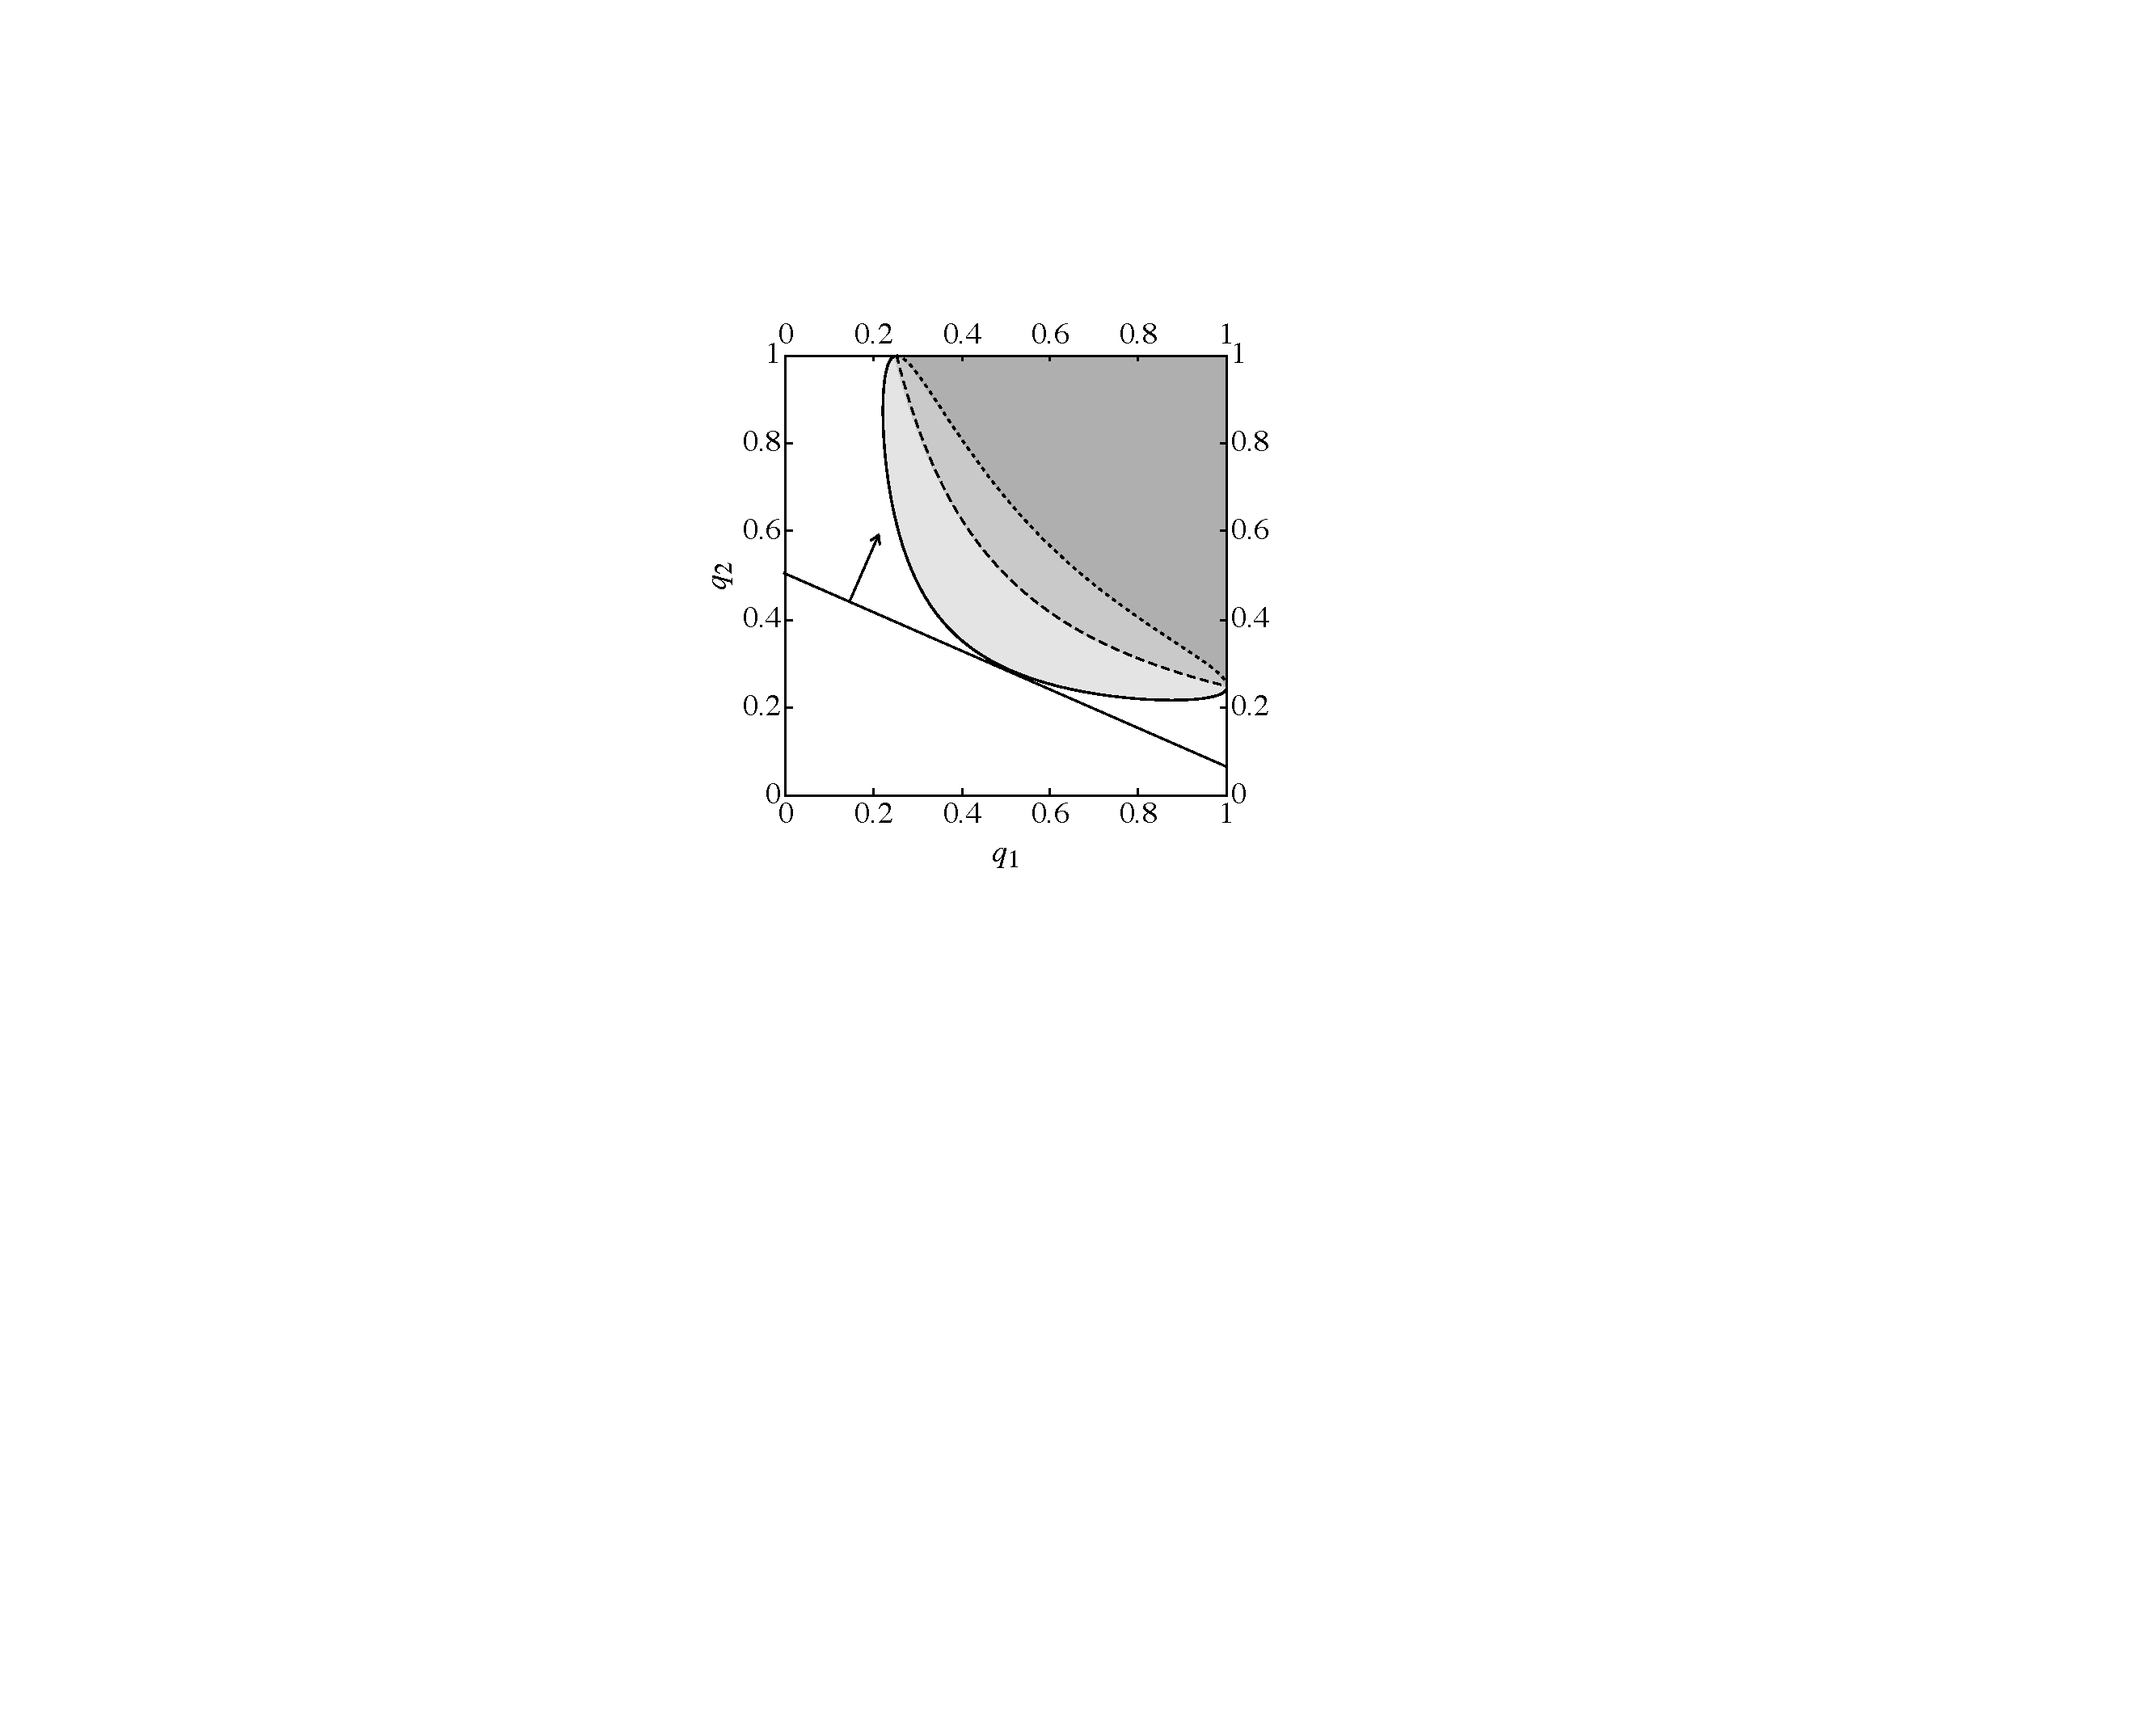
\includegraphics[width=8.5cm,height=8.5cm]{Fig_1NC.pdf}
\protect\caption[\hspace{1cm}Unitarity curves ]{ Unitarity curves in Eq.~(\ref{unit cond}) and the associated sets~$S_{\alpha}$
in Eq.~(\ref{S_alpha}) for values of $\alpha$ positive (solid/light~gray),
zero (dashed/medium gray), and negative (dotted/dark gray). The figure
also shows the optimal straight segment %
\mbox{%
$Q=\eta_{1}q_{1}+\eta_{2}q_{2}$%
} and its normal vector~$(\eta_{1},\eta_{2})$. Plotted for $s=0.5$,
$m=1$, $n=2$, $\alpha=0.8,0,-0.8$.}
\label{fig:1} 
\end{figure}


Before attempting to minimize $Q$, we need to gain geometric insight
into the meaning of the unitary constraint. The following points turn
out to be important: (a)~For fixed $s$, $N$ and $M$ Eq.~(\ref{unit cond})
defines a class of smooth curves on the unit square $0\le q_{i}\le1$
(e.g., solid, dashed or dotted curves in Fig.~\ref{fig:1}). (b)~All
these curves meet at their endpoints, $(1,s^{2M})$ and $(s^{2M},1)$.
(c)~At the endpoints the curves become tangent to the vertical and
horizontal lines~$q_{1}=1$ and~$q_{2}=1$ respectively, provided~$\alpha\not=0$.
%This is due to the square root $\sqrt{p_1p_2}$ in Eq.~(\ref{unit cond}).%A more detailed analysis shows that f(d)~For~$\alpha=0$
the curve %defined by Eq.~(\ref{unit cond}) is an arc of the hyperbola
$q_{1}q_{2}=s^{2M}$ (dashed line in Fig.~\ref{fig:1}). (e)~Each
of these curves and the segments joining their end points with the
vertex~$(1,1)$ are the boundary of the sets (any of the gray regions
in Fig.~\ref{fig:1}) 
\begin{equation}
S_{\alpha}=\{(q_{1},q_{2}):\sqrt{p_{1}p_{2}}\,s^{N}\alpha+\sqrt{q_{1}q_{2}}-s^{M}\ge0\}.\label{S_alpha}
\end{equation}
They satisfy $S_{\alpha}\subset S_{\alpha'}$ if $\alpha<\alpha'$.
(f)~Moreover, the sets~$S_{\alpha}$ are convex if $\alpha\ge0$.
In particular $S_{1}$ is convex. %For $\alpha\ge0$ the set $S_\alpha$ is convex, as follows from the observation that~$(xy)^{1/2}$ is a concave function of its two (non-negative) arguments~$x$ and~$y$. 

At this point a geometrical picture of the optimization problem emerges
(See Fig.~\ref{fig:1}). Eq.~(\ref{obj fun}) defines a straight
segment on the square $0\le q_{i}\le1$ with a normal vector in the
first quadrant parallel to $(\eta_{1},\eta_{2})$. For fixed prior
probabilities, the average failure probability~$Q$ is proportional
to the distance from this segment to the origin~$(0,0)$. Since $S_{1}$
is convex and the stretch of its boundary given by Eq.~(\ref{unit cond})
with $\alpha=1$ is smooth, a unique point $(q_{1},q_{2})$ of tangency
with the segment~(\ref{obj fun}) exists for any value of the priors
and finite $N$. It gives $Q_{{\rm min}}$ and defines the optimal
cloning strategy. %(See Fig.~\ref{fig:1}). 

We note in passing that the inclusion hierarchy of the sets $S_{\alpha}$
provides a simple geometrical proof that $\alpha=1$, i.e., $|\alpha_{1}\rangle=|\alpha_{2}\rangle$,
is indeed the optimal choice. On the other hand, we recall that for
cloning by discrimination we have $\langle\alpha_{1}|\alpha_{2}\rangle=\alpha=0$.
From points~(b) and~(c) above, it follows that for any finite $N$
and arbitrary priors $\eta_{1}$ and $\eta_{2}$ this protocol is
strictly suboptimal, i.e., $Q_{{\rm min}}<Q_{{\rm UD}}$, where the
subscript UD is a reminder that the failure rate of cloning by discrimination
is that of UD. One could say that optimal cloning is incompatible
with discerning the identity of the input states for any finite number
of clones. However, optimal cloning and UD become one and the same
in the limit $N\to\infty$, where $s^{N}\to0$ and the curve~(\ref{unit cond})
collapses to the hyperbola $q_{1}q_{2}=s^{2M}$, as it does for $\alpha=0$.
We will come back to this point below. A more quantitative analysis
requires finding a convenient parametrization of the curve~(\ref{unit cond}).
To this end, simpler and more manageable expressions are derived if
the symmetry under $q_{1}\leftrightarrow q_{2}$ is preserved. We
write $\sqrt{q_{i}}=\sin\theta_{i}$ for $0\leq\theta_{i}\leq\pi/2$.
By further introducing the variables $x=\cos(\theta_{1}+\theta_{2})$
and $y=\cos(\theta_{1}-\theta_{2})$ we manage to linearize the constraint~(\ref{unit cond}),
which now reads as $2s^{M}=(1+s^{N})y-(1-s^{N})x$. A natural parametrization
for this straight line is given by 
\begin{equation}
x=\frac{1-(1+s^{N})t}{s^{N-M}},\qquad y=\frac{1-(1-s^{N})t}{s^{N-M}},\label{x =000026 y}
\end{equation}
where again we have taken the most symmetrical choice. Because of
the symmetry of this procedure, the parameters $x$ and $y$ are invariant
under $q_{1}\leftrightarrow q_{2}$ (equivalently, under $\theta_{1}\leftrightarrow\theta_{2}$).
Thus, the two mirror halves of the curve~(\ref{unit cond}) under
this transformation are mapped into the same straight line~(\ref{x =000026 y}).
By expressing $q_{i}$ as a function of~$t$ only half of the original
curve is recovered. The other half is trivially obtained by applying~$q_{1}\leftrightarrow q_{2}$.

The allowed domain of $t$ in Eq.~(\ref{x =000026 y}) follows from
that of~$x$ and~$y$, readily seen from their definition to be
the region $|x|\le y\le1$. Hence, we have 
\begin{equation}
\frac{1-s^{n-m}}{1-s^{n}}\le t\le1.\label{range t}
\end{equation}
After putting the various pieces together one can easily get rid of
the trigonometric functions and express Eq.~(\ref{unit cond}) in
parametric form as 
\begin{equation}
q_{i}=\frac{1-xy-(-1)^{i}\sqrt{1-x^{2}}\sqrt{1-y^{2}}}{2},\quad i=1,2.\label{par sqrt}
\end{equation}
Fig.~\ref{fig:2} shows examples of the unitary curve~(\ref{unit cond})
for (a)~$n=2$ and (b)~$n=5$. In both cases $m=1$. For larger
$n$ the curves closely approximate the hyperbolae $q_{1}q_{2}=s^{2m}$
(dashed lines) for small and moderate values of $s$, while for $s$
close to one the hyperbolas remain closer to the vertex~$(1,1)$,
but still retain the same end points. As mentioned previously, in
the limit $n\to\infty$ all curves become hyperbolic. 
\begin{figure}[hh]
\centering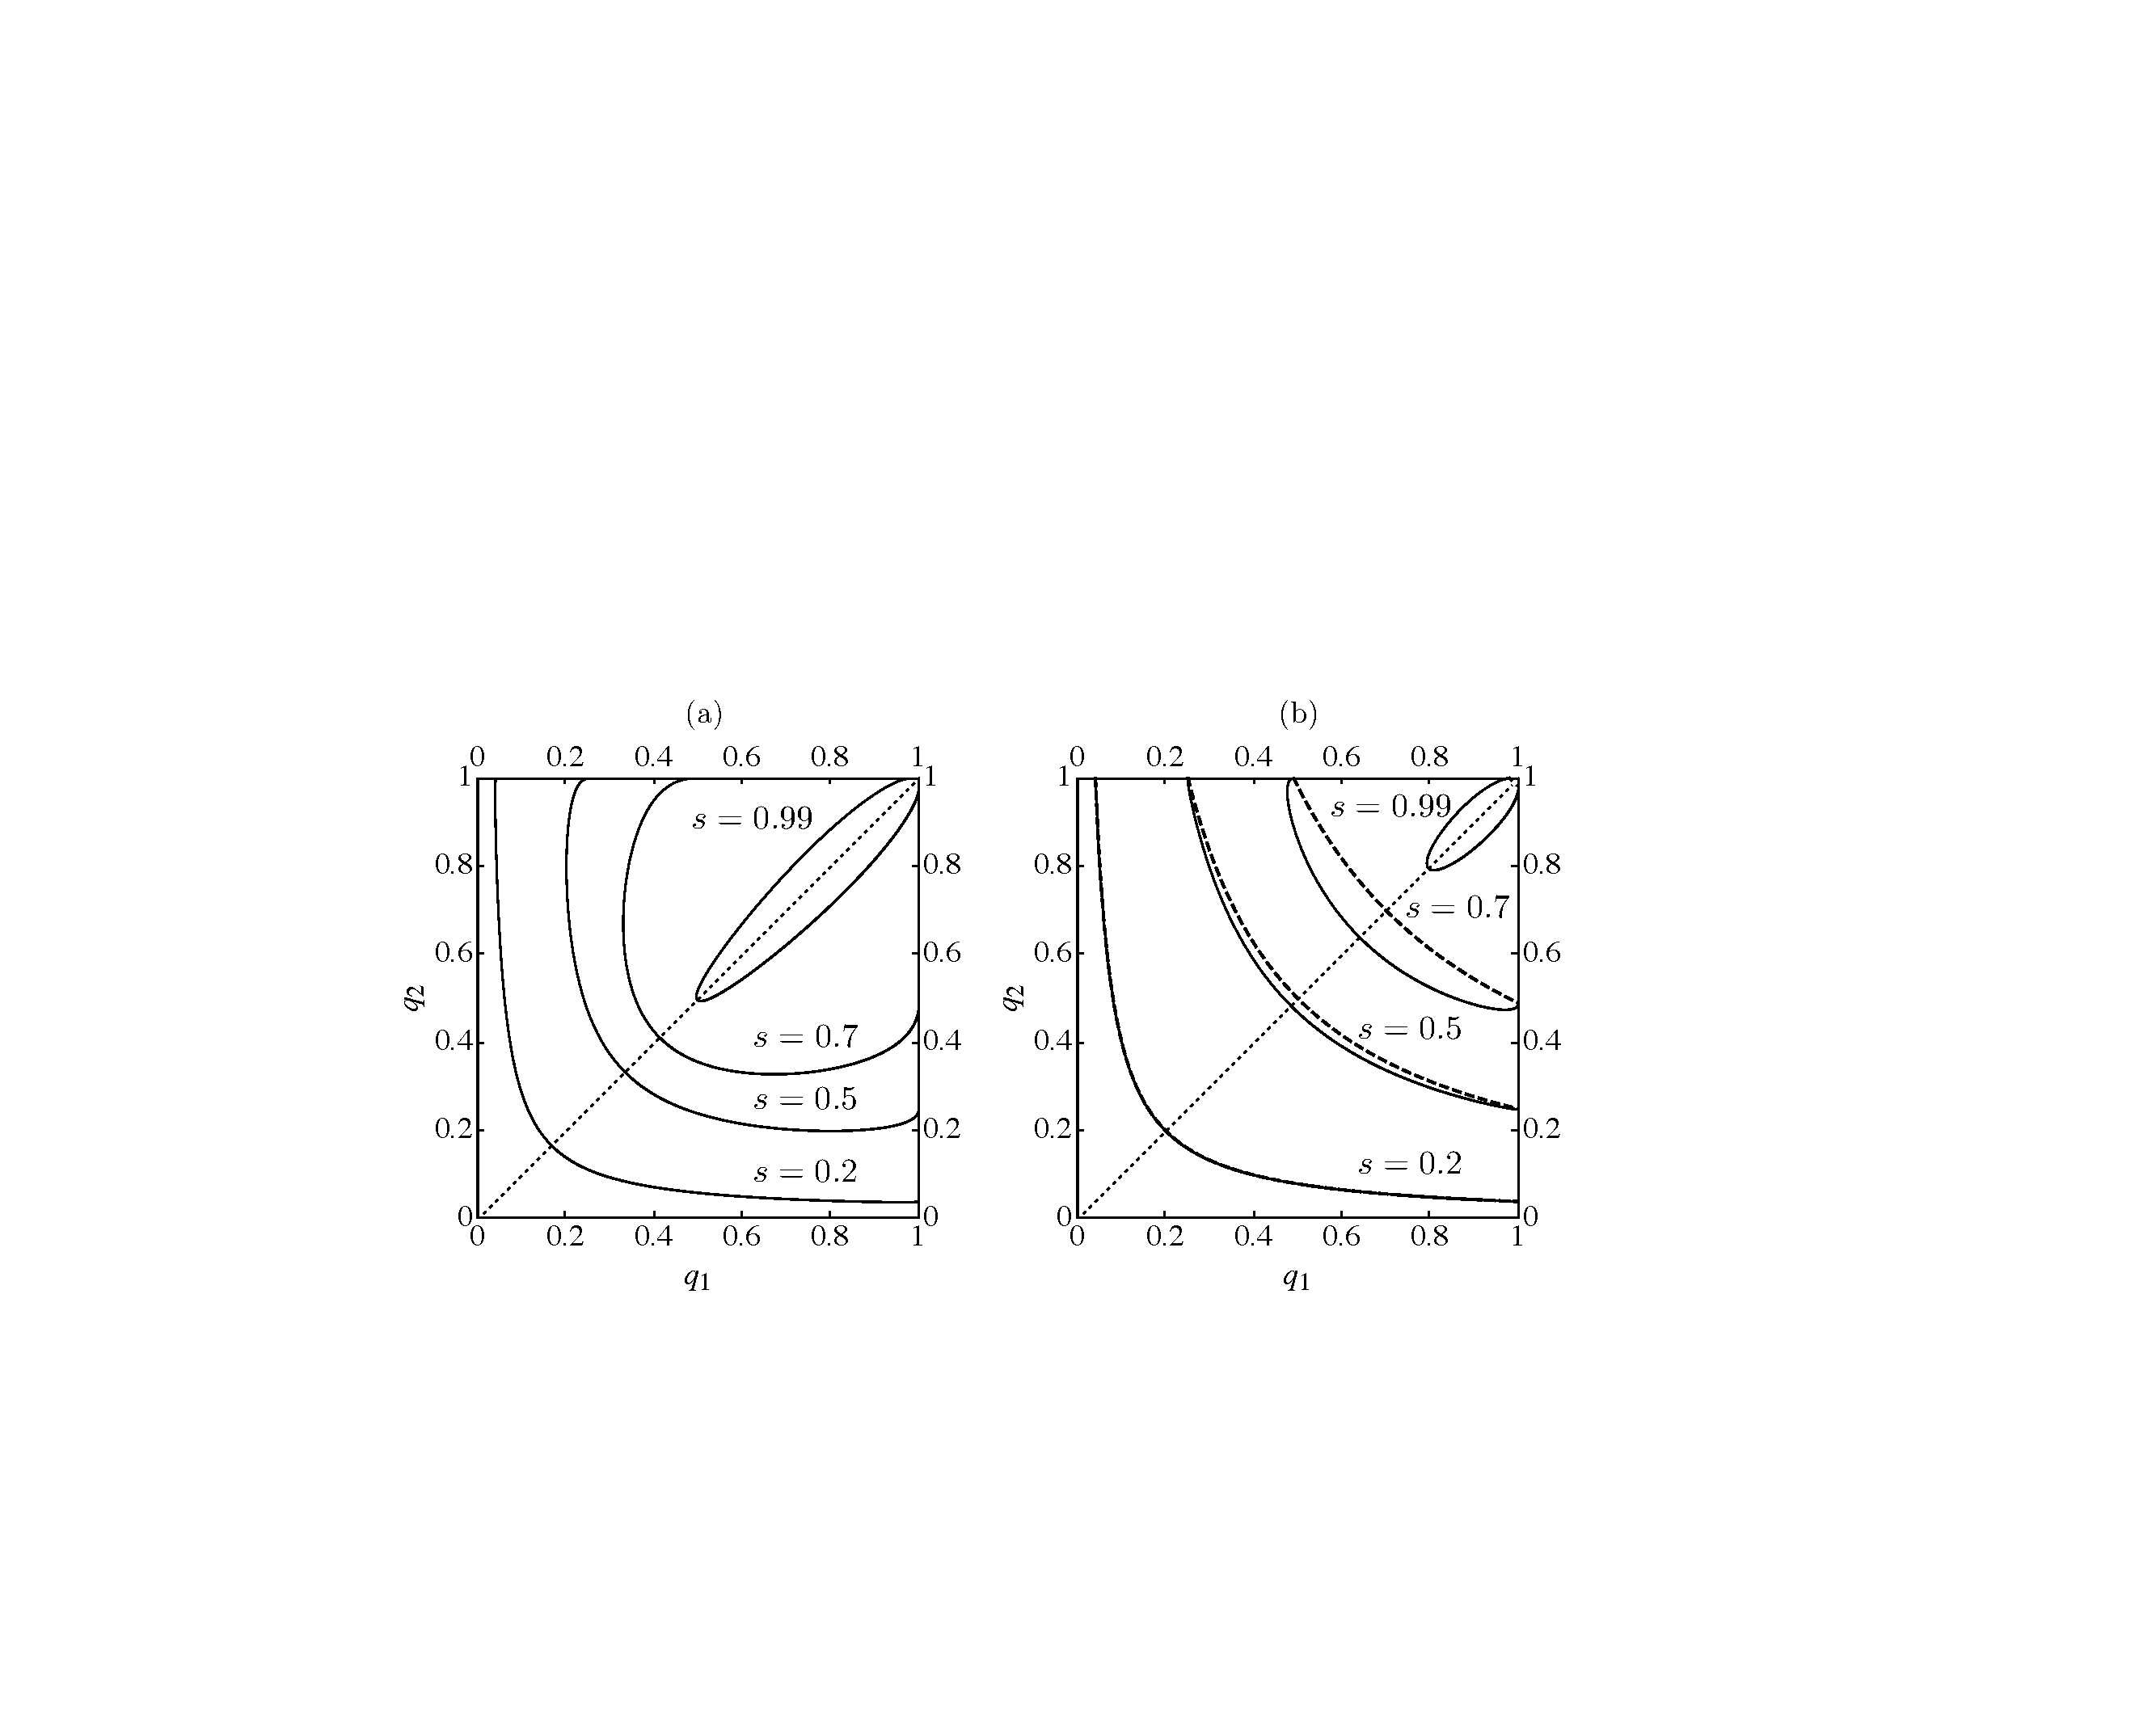
\includegraphics[width=8.5cm,height=8.5cm]{Fig_2NC.pdf}
\protect\caption[\hspace{1cm}Unitarity curves for s ]{ Unitarity curves for different values of~$s$ and for (a) $m=1$,
$n=2$ and (b) $m=1$, $n=5$. The curves are symmetric under mirror
reflexion along the (dotted) straight line $q_{1}=q_{2}$, i.e., under
the transformation~$q_{1}\leftrightarrow q_{2}$. The dashed lines
in~(b) are the hyperbolae~$q_{1}q_{2}=s^{2m}$.}
\label{fig:2} 
\end{figure}


Now we can return to the minimization of the average failure probability
$Q$. Despite the apparent simplicity of the problem, finding the
minimum $Q$ as an explicit function of $\eta_{1}$ or $\eta_{2}$
involves solving a quartic equation without a simple form~ Instead,
we will derive the parametric equation of the curve $(\eta_{1},Q_{{\rm min}})$.
This, along with our complete description of the unitary curve~,
provides a full account of the solution.

Without any loss of generality we may assume that~$\eta_{1}\le\eta_{2}$,
or equivalently, that~$0\le\eta_{1}\le1/2$. Then the slope of the
vector normal to the straight line~(\ref{obj fun}) is less or equal
to one and thus it can only become tangent to the lower half of the
unitary curve~(\ref{unit cond}) (see Fig.~\ref{fig:2}). The slope
of this lower half increases monotonically as we move away from the
line~$q_{1}=q_{2}$, where it has the value~$-1$, and vanishes
before we reach the line~$q_{1}=1$. This follows from the properties
(a)--(f) above and can be checked using Eq.~(\ref{par sqrt}). The
values of $t$ at which the slope is $-1$ and $0$ are respectively
\begin{equation}
t_{-1}=\frac{1-s^{n-m}}{1-s^{n}},\quad t_{0}=\frac{1-s^{2(n-m)}}{1-s^{2n}},\label{t's}
\end{equation}
where we note that $t_{-1}$ is the lower value of the range of~$t$
in Eq.~(\ref{range t}). For any point $(q_{1}(t),q_{2}(t))$ with
$t\in[t_{-1},t_{0}]$ there is a line $Q=\eta_{1}q_{1}+\eta_{2}q_{2}$
that is tangent to it, starting with $\eta_{1}=\eta_{2}=1/2$ for
$t=t_{-1}$ up to $\eta_{1}=0$, $\eta_{2}=1$ for $t=t_{0}$.

This observation enables us to derive the desired parametric expression
for the optimality curve~$(\eta_{1},Q_{{\rm min}})$ as follows:
for a given $t$ in the range above, a necessary condition for tangency
is %
\mbox{%
$\eta_{1}q'_{1}+\eta_{2}q'_{2}=0$%
}, where $q'_{i}=dq_{i}/dt$. In this equation we can solve for $\eta_{1}$
(or $\eta_{2}$) using that~$\eta_{1}+\eta_{2}=1$. By substituting
$q_{1}$ and~$q_{2}$ in Eq.~(\ref{obj fun}) with~(\ref{par sqrt})
we enforce contact with the unitarity curve and obtain the expression
of $Q_{{\rm min}}$. The final result can be cast as: 
\begin{equation}
\eta_{1}=\frac{q'_{2}}{q'_{2}-q'_{1}},\;\;Q_{{\rm min}}=\frac{q'_{2}q_{1}-q'_{1}q_{2}}{q'_{2}-q'_{1}},\;\;t_{-1}\le t\le t_{0},\label{main}
\end{equation}
where $t_{-1}$, $t_{0}$ and $q_{i}$ are given in Eqs.~(\ref{t's})
and~(\ref{par sqrt}). The expressions for the derivatives $q'_{i}$
are %most easily derived from the trigonometric form~(\ref{par trig}) to be
\begin{equation}
q'_{i}=\frac{\sqrt{q_{i}(1-q_{i})}}{s^{n-m}}\left\{ \frac{1+s^{n}}{\sqrt{1-x^{2}}}-(-1)^{i}\frac{1-s^{n}}{\sqrt{1-y^{2}}}\right\} .
\end{equation}
Fig.~\ref{fig:3} shows plots of the curves $(\eta_{1},Q_{{\rm min}})$
for $m=1$ input copies and (a) $n=2$ or (b) $n=5$ clones, as in
the previous figure. We see that $Q_{{\rm min}}$ is an increasing
function of $\eta_{1}$ in the given range $[0,1/2]$. The values
of~$Q_{{\rm min}}$ at the end points of this range follow by substituting
$t_{0}$ and $t_{-1}$, Eq.~(\ref{t's}), into Eq.~(\ref{par sqrt}).
They are given by 
\begin{equation}
Q_{0}=q_{2}(t_{0})=\frac{s^{2m}-s^{2n}}{1-s^{2n}},\quad Q_{-1}=\frac{s^{m}-s^{n}}{1-s^{n}},\label{Q's}
\end{equation}
where $Q_{{\rm min}}=Q_{-1}$ holds for equal priors and $Q_{{\rm min}}=Q_{0}$
for $\eta_{1}\to0$ (i.e., $\eta_{2}\to1$). 
\begin{figure}[h]
\centering 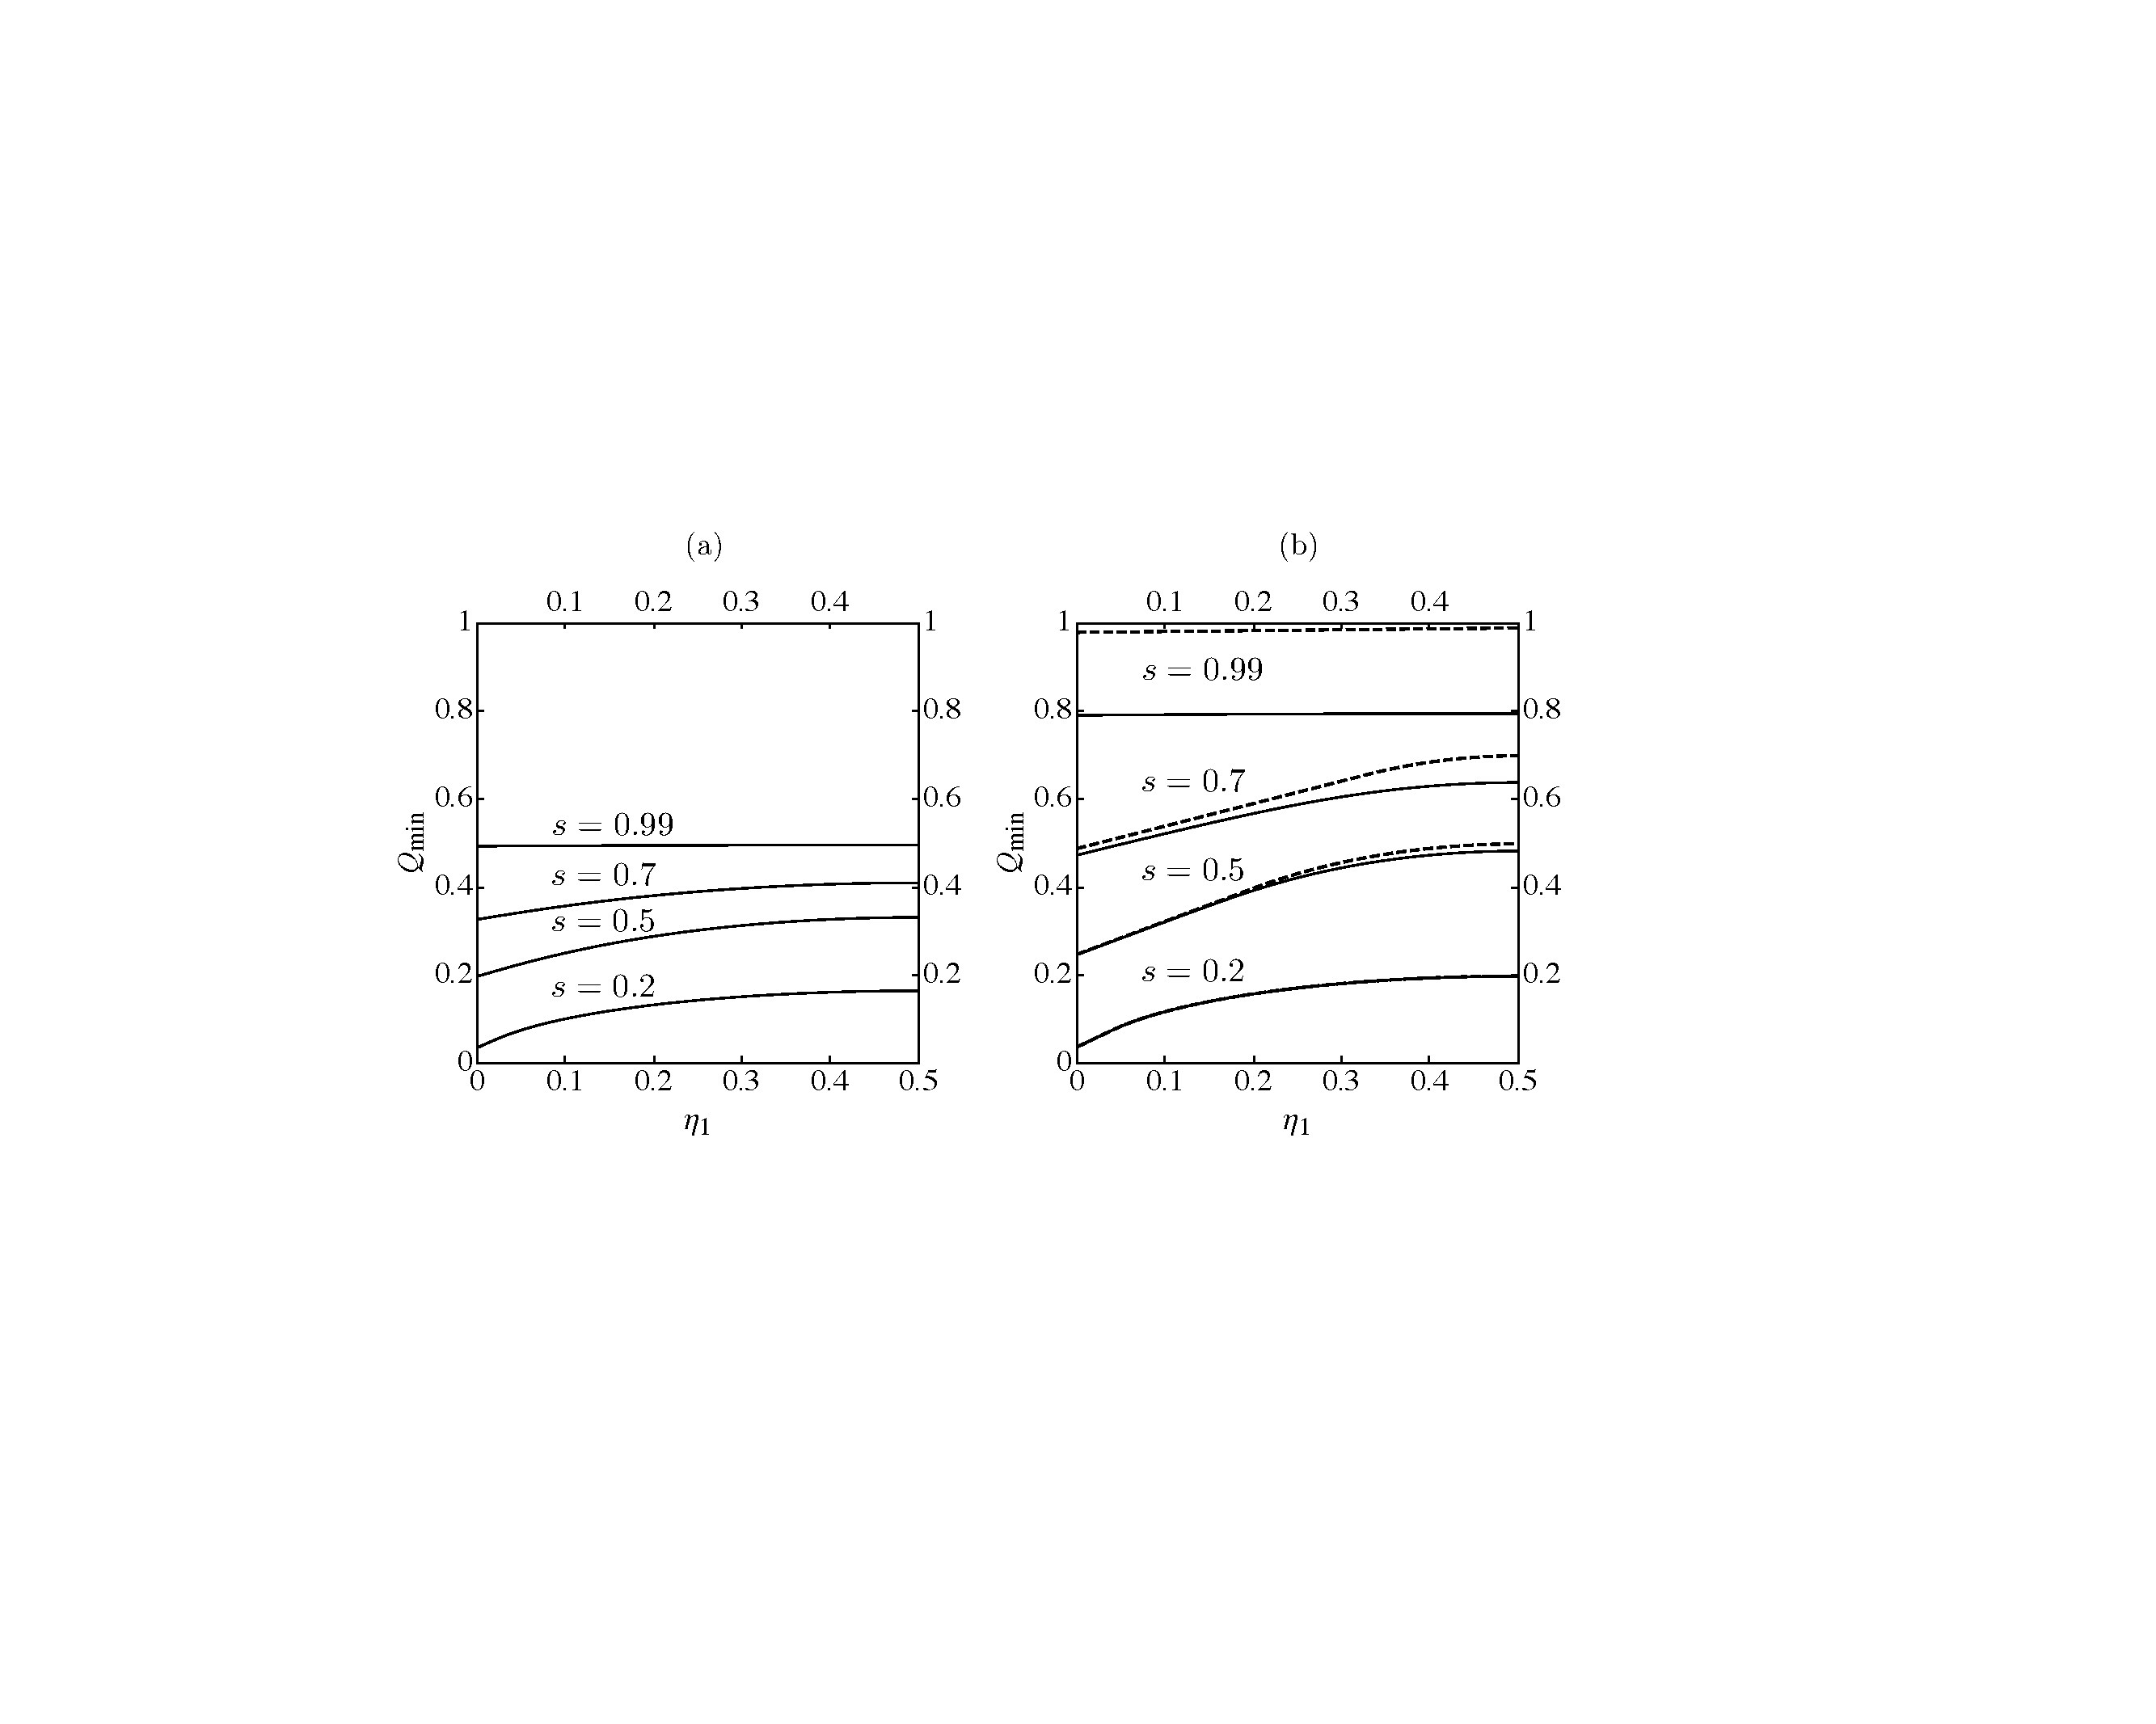
\includegraphics[width=8cm,height=6cm]{Fig_3NC.pdf}\protect\caption[\hspace{1cm}$Q_{{\rm min}}$ vs. $\eta_{1}$ ]{ Minimum cloning failure probability $Q_{{\rm min}}$ vs. $\eta_{1}$
(solid lines) and~UD failure probability $Q_{{\rm UD}}$ vs. $\eta_{1}$
(dashed lines) for the same values of $m$, $n$ and $s$ used in
the previous figure.}
\label{fig:3} 
\end{figure}
The dashed lines in Fig.~\ref{fig:3}~(b) are the well known piecewise
unambiguous discrimination solution~\cite{Bergou2010}: 
\begin{equation}
Q_{{\rm UD}}=\left\{ \begin{array}{ll}
\eta_{1}+s^{2m}\eta_{2},\quad & {\displaystyle 0\le\eta_{1}\le\frac{s^{2m}}{1+s^{2m}};}\\[0.5em]
2\sqrt{\eta_{1}\eta_{2}}\,s^{m}, & {\displaystyle \frac{s^{2m}}{1+s^{2m}}\le\eta_{1}\le\frac{1}{2}.}
\end{array}\right.\label{UD-1}
\end{equation}
It is apparent from these plots that the optimal cloning protocol
performs strictly better than cloning by discrimination, as was proved
above. However, as the number of produced clones becomes larger the
difference in performance reduces. In Fig.~\ref{fig:3}~(b), for
only $n=5$, a difference is hardly noticeable for $s\le0.5$. For
larger overlaps it takes larger values of $n$ to get the same level
of agreement. As discussed above, in the limit $n\to\infty$ there
is perfect agreement for any $s<1$.

The complete UD solution in Eq.~(\ref{UD-1}) emerges naturally from
our geometrical approach in a straightforward manner: First, we recall
that in this case the right hand side of Eq.~(\ref{unit cond}) becomes
$q_{1}q_{2}=s^{2m}$ (dashed lines in Figs.~\ref{fig:1} and~\ref{fig:2}).
The maximum slopes of these curves are at their end points and all
have the value~$-s^{2m}$. This implies that the boundary of $S_{0}$
has a cusp at $(1,s^{2m})$. It follows that a unique point of tangency
with the line~(\ref{obj fun}) exists for $s^{2m}<\eta_{1}/\eta_{2}\le1$
(recall that we are assuming~$\eta_{1}\le1/2$). This condition gives
the $\eta_{1}$ interval for that solution. The tangency condition,
$(q_{2},q_{1})\propto(\eta_{1},\eta_{2})$, quickly leads us to the
optimal failure rate in the second line of Eq.~(\ref{UD-1}). For
$s^{2m}>\eta_{1}/\eta_{2}\ge0$ tangency is not possible, and the
optimal line~(\ref{obj fun}) merely touches the cusp on the boundary
of~$S_{0}$, so the expression of $Q$ becomes the first line of
Eq.~(\ref{UD-1}). In geometrical terms, the straight line~(\ref{obj fun})
pivots on the end point as $\eta_{1}$ varies between $0$ and $s^{2m}/(1+s^{2m})$.

For the second case in Eq.~(\ref{UD-1}), one has $q_{1},p_{1}\in(0,1)$
and there are three orthogonal flag states in Eqs.~(\ref{Ui}), namely,
the two success states $|\alpha_{1}\rangle$, $|\alpha_{2}\rangle$,
and the failure state~$|\Phi\rangle$. This $3$-outcome measurement
can be represented by a $3$-element positive operator valued measure
(POVM) on ${\mathscr{H}}^{\otimes m}$. For the first line in Eq.~(\ref{UD-1}),
$p_{1}=1-q_{1}=0$, which leads to a $2$-outcome projective measurement,
as only one success flag state ($|\alpha_{2}\rangle$) is needed in
Eqs.~(\ref{Ui}).

This two-paragraph derivation of Eq.~(\ref{UD-1}) proves that the
convergence of the optimal cloning failure probability~$Q_{{\rm min}}$
to that of cloning by discrimination, with rate $Q_{{\rm UD}}$ in
Eq.~(\ref{UD-1}), follows from the convergence of the general unitarity
curve in Eq.~(\ref{unit cond}) to the hyperbola $q_{1}q_{2}=s^{2m}$,
i.e., from $\lim_{\alpha\to0}S_{\alpha}=S_{0}$. Interestingly enough,
such convergence entails a phenomenon analogous to a second order
phase transition. Our geometrical approach shows that the average
failure probability $Q_{{\rm min}}(\eta_{1})$ is an infinitely differentiable
function of~$\eta_{1}$ for finite $n$. However, as $n$ goes to
infinity (or at $\alpha=0$, for the sake of this discussion) the
limiting function $Q_{{\rm UD}}(\eta_{1})$ has a discontinuous second
derivative. Moreover, the symmetry $q_{1}\leftrightarrow q_{2}$ breaks
in the phase corresponding to the first line in Eq.~(\ref{UD-1}).
A~similar phenomenon arises in UD of more than two pure states~\cite{Bergou2012}
.

It has been argued above that cloning by discrimination is strictly
suboptimal (unless $n\to\infty$). One could likewise wonder if discrimination
by cloning can be optimal. On heuristic grounds, one should not expect
this to be so, as cloning involves a measurement and some information
can be drawn from the observed outcome. However, the equal-prior and
the $\eta_{1}\to0$ cases provide remarkable exceptions. For both
we may write the total failure rate as $Q_{{\rm C}}+(1-Q_{{\rm C}})Q_{{\rm UD}}$,
where C stands for cloning. For $\eta_{1}=\eta_{2}=1/2$, Eq.~(\ref{Q's})
implies $Q_{{\rm C}}=Q_{-1}$, in which case the produced $n$-clone
states are equally likely. The UD of these states fails with probability
$s^{n}$, as follows from Eq.~(\ref{UD-1}) applied to $n$ copies.
The total failure rate is then $s^{m}$, which is the optimal UD failure
rate of the original input states, Eq.~(\ref{UD-1}). If $\eta_{1}\to0$
then only $|\psi_{2}^{n}\rangle$ is produced with non-vanishing probability
and $Q_{{\rm C}}=Q_{0}$. Failure in the second step (UD) is given
by the top line in Eq.~(\ref{UD-1}) applied to $n$ copies. The
total failure rate is $s^{2m}$, also achieving optimality.

Using our main result in Eqs.~(\ref{main}), and~(\ref{par sqrt})
one can check that these are the only cases where discrimination by
cloning is optimal. These are also the only cases where no information
gain can be drawn from the cloning measurement. This hints at how
special these cases are and justifies the need of the derived solution
for arbitrary priors to have a full account of two-state cloning.

%%%%%%%%%%%%%%%%%%%%%%%%%%%%%%%%%%%%%%%%%%%%%%%%
%%%%%%%%%%%%%%%%%%%%%%%%%%%%%%%%%%%%%%%%%%%%%%%%
\subsection{Unequal priors II}

In this section we show a different geometric/numeric solution using
the Lagrange multipliers method with the constraint given in Equation
(\ref{eq:clone overlap}), 

\begin{equation}
s=\sqrt{(1-q_{1})(1-q_{2})}s^{2}+\sqrt{q_{1}q_{2}},\label{eq:1 to 2 cloning constraint}
\end{equation}
where we set $M=1,$ $N=2$ for notation simplicity. This corresponds
to one to two cloning but can be easily generalized for $M$ to $N$
cloning, $M\geq N$ . The function to be maximized is:

\begin{equation}
F_{S}=\eta_{1}q_{1}+\eta_{2}q_{2}+\lambda\left[s-\sqrt{\left(1-q_{1}\right)\left(1-q_{2}\right)}s^{2}-\sqrt{q_{1}q_{2}}\right],
\end{equation}
where $\lambda$ is the Lagrange multiplier to be determined which
optimizes the failure rate $Q=\eta_{1}q_{1}+\eta_{2}q_{2}.$ Set $\partial F/\partial q_{i}=0$,
solve for $q_{i}$,

\begin{eqnarray}
\frac{2\eta_{1}}{\lambda} & = & \sqrt{\frac{q_{2}}{q_{1}}}-\sqrt{\frac{1-q_{2}}{1-q_{1}}}s^{2},\label{eq:lagr1}\\
\frac{2\eta_{2}}{\lambda} & = & \sqrt{\frac{q_{1}}{q_{2}}}-\sqrt{\frac{1-q_{1}}{1-q_{2}}}s^{2}.\label{eq:lagr2}
\end{eqnarray}


Let $A\equiv\sqrt{\frac{q_{2}(1-q_{1})}{q_{1}(1-q_{2})}},$ 

\begin{eqnarray}
\sqrt{\frac{q_{1}}{q_{2}}} & = & \frac{\lambda}{2\eta_{1}}\left[1-\frac{s^{2}}{A}\right],\\
\sqrt{\frac{q_{2}}{q_{1}}} & = & \frac{\lambda}{2\eta_{2}}\left[1-As^{2}\right],
\end{eqnarray}
Multiplying the above two equations, setting $\delta=\frac{4\eta\eta_{2}}{\lambda^{2}}$
and $C=\frac{s^{4}-\delta+1}{s^{2}}$ results in a quadratic equation:

\begin{eqnarray}
\delta-1 & = & s^{2}\left[s^{2}-A-\frac{1}{A}\right],\nonumber \\
0 & = & A^{2}-CA+1.\label{eq:QuadratinA1}
\end{eqnarray}
It is the quadratic equation in (\ref{eq:QuadratinA1}) with the combination
of a second emerging quadratic equation we will use to obtain the
value of $\lambda.$ 

Another quadratic equation emerges using the two equations in (\ref{eq:lagr1})
and (\ref{eq:lagr2}). First let $\alpha\equiv\frac{\lambda}{2\eta_{1}}[1-\frac{s^{2}}{A}]$
and $\frac{1}{\alpha}=\frac{\lambda}{2\eta_{2}}[1-As^{2}]$ the relationship
between the two failure rates becomes:

\begin{equation}
\sqrt{q_{1}}=\alpha\sqrt{q_{2}}.\label{eq:q12}
\end{equation}
Using the relationship in (\ref{eq:q12}) and the definition of $A$,
$q_{i}$ can be expressed explicitly in terms of the fixed constants:
$\{\eta_{1},\eta_{2},s\}$ and the parameter $\lambda$ which is yet
to be determined. The derivation starts from the definition of $A,$

\begin{eqnarray*}
A^{2} & = & \frac{q_{2}\left(1-q_{1}\right)}{q_{1}\left(1-q_{2}\right)},\\
\frac{q_{1}}{1-q_{1}}A^{2} & = & \frac{q_{2}}{1-q_{2}},\\
\frac{\alpha^{2}q_{2}}{1-\alpha^{2}q_{2}}A^{2} & = & \frac{q_{2}}{1-q_{2}}.
\end{eqnarray*}
 Solving for $q_{2}$ then using the relationship $q_{1}=\alpha^{2}q_{2}$
we get:

\begin{eqnarray}
q_{2} & = & \frac{1-\alpha^{2}A^{2}}{\alpha^{2}\left(1-A^{2}\right)},\\
q_{1} & = & \frac{1-\alpha^{2}A^{2}}{\left(1-A^{2}\right)}.
\end{eqnarray}
This is the expression of the individual failure rates which are yet
to be optimized subject to the constraint. Now $q_{1}$ and $q_{2}$
is replaced in the constraint given in (\ref{eq:1 to 2 cloning constraint})
and from there the optimal value of $\lambda$ can be obtained. 

Some prior calculations before replacing $q_{i}$ into the constraint
will simplify the overall algebra:

\[
1-q_{1}=\frac{A^{2}\left(\alpha^{2}-1\right)}{\left(1-A^{2}\right)},
\]


\[
1-q_{2}=\frac{\alpha^{2}-1}{\alpha^{2}\left(1-A^{2}\right)}.
\]


Now we are ready to replace $q_{i}$ and $1-q_{i}$ into the constraint
(\ref{eq:1 to 2 cloning constraint}):

\begin{eqnarray*}
s & = & \frac{A\left(\alpha^{2}-1\right)}{\alpha\left(1-A^{2}\right)}s^{2}+\frac{1-\alpha^{2}A^{2}}{\alpha\left(1-A^{2}\right)},\\
\left(1-A^{2}\right)s & = & \frac{1}{\alpha}\left(1-s^{2}A^{2}\right)-\alpha A^{2}\left(1-\frac{s^{2}}{A}\right),\\
\left(1-A^{2}\right)s & = & \frac{\lambda}{2\eta_{2}}\left(1-s^{2}A^{2}\right)^{2}-\frac{\lambda A^{2}}{2\eta_{1}}\left(1-\frac{s^{2}}{A}\right)^{2}.
\end{eqnarray*}
Here we replaced $\text{ \ensuremath{\alpha}=\ensuremath{\frac{\lambda}{2\eta_{1}}\left[1-\frac{s^{2}}{A}\right]} and \ensuremath{\frac{1}{\alpha}}=\ensuremath{\frac{\lambda}{2\eta_{2}}\left[1-As^{2}\right]}}.$
After some trivial algebra the second quadratic equation in $A$ emerges:

\begin{equation}
A^{2}-\frac{2s^{2}(\eta_{1}-\eta_{2})}{\eta_{1}s^{4}-\eta_{2}+2\eta_{1}\eta_{2}s/\lambda}A+\frac{\eta_{1}-\eta_{2}s^{4}+2\eta_{1}\eta_{2}s/\lambda}{\eta_{1}s^{4}-\eta_{2}+2\eta_{1}\eta_{2}s/\lambda}=0\label{eq: 2nd quadratic in A}
\end{equation}


The combination of Eq. (\ref{eq:QuadratinA1}) and Eq. (\ref{eq: 2nd quadratic in A})
should give the value of $\lambda$ which in turn gives explicit solution
to the minimum individual failure rates, $q_{i},$ and overall optimal
failure rate $Q=\eta_{1}q_{1}+\eta_{2}q_{2}.$ Analytically such a
solution is hard to achieve as one would have to solve a sixth order
equation. Simply by plotting the two quadratic equations as a function
of $\lambda$ the solution can be obtained at the intersection of
the two graphs. There will be multiple intersections, hence multiple
values of $\lambda.$ The one which gives the lowest value of the
overall failure rate is chosen. 
%
%\includegraphics[bb = 0 0 200 100, draft, type=eps]{/Users/ashehu/Desktop/intersect(A1, A2).jpg}
%


In our future work we would like to obtain a closed form solution
of $q_{i}.$ One approach could be by making some educated guess for
$\lambda.$



%%%%%%%%%%%%%%%%%%%%%%%%%%%%%%%%%%%%%%%%%%%%%%%%
%%%%%%%%%%%%%%%%%%%%%%%%%%%%%%%%%%%%%%%%%%%%%%%%
\section{Exact Cloning then Unambiguous Discrimination. *RENAME* }

It is interesting to see the connection between cloning and state
discrimination of non-orthogonal quantum states. To get a better understanding
we consider the two step process where we first clone then make a
measurement. The other way around, state discrimination first then
cloning is less interesting because once we have succeeded in discriminating
a state we can make as many copies as we wish by simply preparing
them with the knowledge we get from the discrimination step. Making
a clone first and then performing state discrimination gives some
interesting results. For the case when the incoming states are prepared
with equal priors we show that cloning first then performing UD on
the cloned states which come with some new a priori probability $p'$
the overall failure rate reaches the IDP limit. 

\medskip{}


The idea of the two step process is the following: 
\begin{enumerate}
\item Probabilistic Exact Cloning: Given an ensemble of $M$ quantum states
$\{|\psi_{1}\rangle,|\psi_{2}\rangle\}$ produce $N$ exact clones
while allowing for a rate of inconclusive outcomes. 
\item Unambiguous Discrimination: Perform optimal unambiguous discrimination
on the successfully cloned states only, throwing away the failed states. 
\end{enumerate}

\subsection*{Equal priors}
\begin{enumerate}
\item Probabilistic Exact Cloning
\end{enumerate}
We showed in Section (3.2.1) that for equal priors and a set of $M$
copies of two non-orthogonal states we could successfully produce
exact copies with a probability $P_{clone}=\frac{1-s^{M}}{1-s^{N}}.$
The average failure rate, failing to clone a state is $Q_{clone}=1-P_{clone}=\frac{s^{M}-s^{N}}{1-s^{N}}.$ 
\begin{enumerate}
\item Optimal Unambiguous Discrimination
\end{enumerate}
After the input states are sent through the deterministic exact cloning
machines, $N$ states of of the ensemble $\{|\psi_{1}\rangle,\thinspace|\psi_{2}\rangle\}$
come out through the output port. The cloning machine only makes copies
and does not say which state it has made a copy of. The clones are
now sent through an unambiguous discriminating machine to distinguish
the incoming states. Each of the states comes with a probability $P_{clone}=\frac{1-s^{M}}{1-s^{N}}.$ 

The incoming states $\{|\psi_{1}^{N}\rangle_{s},|\psi_{2}^{N}\rangle_{s}\}$
which live in the state Hilbert space $S$ are embedded with the ancilla
$|i\rangle_{a}$ which live in the ancilla Hilbert space $A.$ Now
the system and the ancilla live in the larger Hilbert space $H=S\varotimes A.$
The incoming states in this larger Hilbert space can be written in
the product form $\{|\psi_{1}^{N}\rangle_{s}|i\rangle_{a},|\psi_{2}^{N}\rangle_{s}|i\rangle_{a}\}$ 

\begin{eqnarray}
U|\psi_{1}\rangle^{\oplus N}\ket 0 & = & \sqrt{p}|\phi\rangle_{s}|1\rangle_{a}+\sqrt{q}|\Phi\rangle_{s}|0\rangle_{a}\nonumber \\
U|\psi_{1}\rangle^{\oplus N}\ket 0 & = & \sqrt{p}|\phi^{\perp}\rangle_{s}|2\rangle_{a}+\sqrt{q}|\Phi\rangle_{s}|0\rangle_{a}\label{eq:sep}\\
\nonumber 
\end{eqnarray}
Here $p$ is the probability of successfully discriminating the state
$|\psi_{i}^{N}\rangle_{s}$, $q$ is the probability of failing to
discriminate $|\psi_{i}^{N}\rangle_{s},$ $p+q=1.$ The unitary operator
takes the two incoming states and projects them onto a pair of orthogonal
states with some success and some failure probability. When there
is a click on the ancilla $|1\rangle_{a}$ the input states have been
separated and output states $|\psi'_{i}\rangle_{s}$ are orthogonal
and thus fully distinguishable. If there is a click along the ancilla
$|0\rangle_{a}$ the incoming states have been collapsed into a single
state which carries no information.

The inner product of the two equations in (\ref{eq:sep}) produces
the solution $s^{N}=q.$ In addition one has to take into consideration
the fact that the states come in with a priori probability of $\frac{1}{2}p=\frac{1}{2}\frac{1-s^{M}}{1-s^{N}}$.
The optimal inconclusive rate for discriminating the incoming pair
of states is$Q=\tilde{\eta}_{1}q_{1}+\tilde{\eta}_{2}q_{2}=\eta_{1}p_{1}q_{1}+\eta_{2}p_{2}q_{2}=\frac{1-s^{M}}{1-s^{N}}s^{N}$
, where $q_{1}=q_{2}=s^{N}$ and success rate is $p_{1}=p_{2}=\frac{s^{M}-s^{N}}{1-s^{N}}.$ 

The total inconclusive rate for the two step process, the failure
rate to clone plus failure rate to unambiguously discriminate, is 

\begin{eqnarray}
Q_{total} & = & Q_{clone}+\left(1-Q_{clone}\right)Q_{UD},\nonumber \\
 & = & \frac{s^{M}-s^{N}}{1-s^{N}}+\frac{1-s^{M}}{1-s^{N}}s^{N}=s^{M}.\label{eq:overlap}
\end{eqnarray}


The two step process reaches the IDP limit for optimal UD of $M$
non-orthogonal states. This is a special case and only occurs for
symmetric case when states are prepared with equal prior probabilities. 



%%%%%%%%%%%%%%%%%%%%%%%%%%%%%%%%%%%%%%%%%%%%%%%%
%%%%%%%%%%%%%%%%%%%%%%%%%%%%%%%%%%%%%%%%%%%%%%%%
\section{Hybrid Cloning: Interpolation between exact and approximate cloning }

In this section we seek to interpolate between probabilistic exact
cloning and approximate cloning machines using our results from state
separation. Exact cloning machines produce perfect clones while allowing
for some inconclusive outcomes. Approximate cloning machines produce
copies on demand which resemble the input states by maximizing the
fidelity. One can imagine a scheme where fidelity can be higher then
maximum fidelity in the approximate cloning machine while it allows
for a fixed rate of inconclusive outcomes, FRIO. This scheme should
reproduce exact cloning and approximate cloning machines by setting
FRIO to $Q_{o}$ and zero respectively. Chefles and Barnett \cite{Chefles1999}
solved the problem for the case when the input states are prepared
with equal a priori probabilities. We extend the solution to the more
general case when the states are prepared with different priors. Such
a solution is possible due to our recent work on making $N$ perfect
clones from $M$ copies of one of two known pure states with minimum
failure probability in the general case where the known states have
arbitrary priori probabilities.

%%%%%%%%%%%%%%%%%%%%%%%%%%%%%%%%%%%%%%%%%%%%%%%%
%%%%%%%%%%%%%%%%%%%%%%%%%%%%%%%%%%%%%%%%%%%%%%%%
\subsection{Equal priors}

The solution to the interpolation of cloning for equal a priori probabilities
has been derived by Chefles et al \cite{Chefles1999}. The authors
develop a scheme which, depending on the fidelity of the clones, can
interpolate between exact cloning with inconclusive results in one
extreme and optimal approximate cloning on the other extreme. In our
work this scheme has been generalized for the case when the input
states are prepared with different a priori probabilities. First we
show the derivation of the equal priors as it will help to better
understand the general case. 

For $\eta_{1}=\eta_{2}=1/2,$ the output states are symmetric, $\phi_{1}=\phi_{2}=\phi,$
and the optimal global fidelity, $F_{MN}$, in Eq.(\ref{eq:fid})
reduces to: 

\begin{eqnarray}
F_{MN} & = & \frac{1}{2}\left[1+\sqrt{1-\sin^{2}\left(2\theta-2\phi\right)}\right],\nonumber \\
 & = & \frac{1}{2}\left[1+\cos^{2}\left(2\theta-2\phi\right)\right].\\
\nonumber 
\end{eqnarray}
 

Duan and Guo \cite{Duan1998} showed that the maximum success probability
of obtaining $N$ exact clones from $M$ given copies of non-orthogonal
quantum states $\{|\psi_{1}\rangle,|\psi_{2}\rangle\}$, which are
prepared with equal a priori probabilities, is:

\begin{equation}
P_{MN}=\frac{1-s^{M}}{1-s^{N}},
\end{equation}
where $s$ is the overlap of the input states $s=\langle\psi_{1}|\psi_{2}\rangle.$
The success rate for 1 to 2 cloning, $M=1,N=2,$ reduces to:

\begin{equation}
P_{12}=\frac{1}{1+s}.
\end{equation}
The interpolation takes us from optimal exact cloning to maximum fidelity.
Given a set $K$ of two non-orthogonal quantum states, $\{|\psi_{1}\rangle,|\psi_{2}\rangle\}$
the goal is to make $N$ clones $\{|\phi_{1}\rangle,|\phi_{2}\rangle\}$,
which are similar to the input states but not perfect. The Neumark
setup is:

\begin{eqnarray}
U|\psi_{1}\rangle^{\otimes M}|i\rangle & = & \sqrt{p}|\phi_{1}\rangle^{\oplus N}|1\rangle+\sqrt{q}|f\rangle|0\rangle\label{eq:NeumarkClone1}\\
U|\psi_{2}\rangle^{\oplus M}|i\rangle & = & \sqrt{p}|\phi_{2}\rangle^{\oplus N}|1\rangle+\sqrt{q}|f\rangle|0\rangle\label{eq:NeumarkClone2}
\end{eqnarray}


The input states are prepared with equal a priori probabilities. A
click in the $|1\rangle$ direction means that we succeed in making
the clones and the probability of success is $p.$ A click in the
$|0\rangle$ direction means that we failed to create a clone with
a probability $q.$ The inner product or (\ref{eq:NeumarkClone1})
and (\ref{eq:NeumarkClone2}) gives the constraint: 

\begin{equation}
s^{M}=ps'^{N}+q
\end{equation}


Using the unitarity condition $p+q=1,$ the average rate of successfully
making a clone is:

\begin{equation}
p=\frac{1-s^{M}}{1-s'^{N}}
\end{equation}


$s'$ is the overlap of the clones $s'=\langle\phi_{1}|\phi_{2}\rangle$.
If the final states are orthogonal, $s'=0$ then the state separation
reaches the IDP limit and $P_{S}=P_{IDP}=1-|\langle\psi_{1}|\psi_{2}\rangle|^{M}.$ 

First we express the overlap of the output states in terms on the
success rates and the overlap of input states, $\cos2\theta=|\langle\psi_{1}|\psi_{2}\rangle|^{N}$

\begin{eqnarray}
|\langle\phi_{1}|\phi_{2}\rangle|^{N} & = & 1-\frac{1-|\langle\psi_{1}|\psi_{2}\rangle|^{M}}{P_{S}}\\
\cos^{N}(\phi_{1}+\phi_{2}) & = & 1-\frac{P_{IDP}}{P_{S}}\label{eq:seperation}
\end{eqnarray}
The exact clones live in an N dimensional space $|\psi_{1,2}^{N}\rangle=\cos\theta|1\rangle\pm\sin\theta|0\rangle.$
The approximate clones can be expressed as $|\phi_{1,2}\rangle=\cos\phi_{1}|1\rangle\pm\sin\phi_{1}|0\rangle$.

The fidelity rate for equal priors is:

\begin{equation}
F_{MN}=\frac{1}{2}\left[1+\cos(2\theta-\left(\phi_{1}+\phi_{2}\right)\right],
\end{equation}
 and we want to use the relationship in (\ref{eq:seperation}). Let
us expand the cosine term 

$\cos\left(2\theta-\left(\phi_{1}+\phi_{2}\right)\right)=\cos2\theta\cos\left(\phi_{1}+\phi_{2}\right)+\sin2\theta\sin\left(\phi_{1}+\phi_{2}\right).$

The fidelity becomes:

\begin{eqnarray*}
\\
F_{MN} & = & \frac{1}{2}\left[1+|\langle\psi_{1}^{N}|\psi_{2}^{N}\rangle|\left(1-\frac{P_{IDP}}{P_{S}}\right)+\frac{1}{P_{S}}(\left(1-|\langle\psi_{1}^{N}|\psi_{2}^{N}\rangle|^{2}\right)\left(P_{S}^{2}-\left(P_{S}-P_{IDP}\right)^{2}\right)^{1/2}\right]
\end{eqnarray*}
 As $N\rightarrow\infty,\thinspace|\langle\psi_{1}|\psi_{2}\rangle|^{N}\rightarrow0$
and $F_{MN}$ reduces to

\[
F_{MN}=\frac{1}{2}[1+\frac{1}{P_{S}}\sqrt{P_{S}^{2}-(P_{S}-P_{IDP})^{2}}].
\]


We can also express the fidelity in terms of fixed failure rate $Q=1-P_{S}$
which serves as the parameter by which we are interpolating and the
optimal failure rate $Q_{o}=\left|\langle\psi_{1}|\psi_{2}\rangle\right|$ 

\begin{eqnarray*}
F_{MN} & = & \frac{1}{2}\left[1+|\langle\psi_{1}^{N}|\psi_{2}^{N}\rangle|(1-\frac{1-Q_{o}}{1-Q})+\frac{1}{1-Q}(\left(1-|\langle\psi_{1}^{N}|\psi_{2}^{N}\rangle|^{2}\right)\left(\left(1-Q\right)^{2}-(Q-Q_{o})^{2}\right)^{1/2}\right],\\
 & = & \frac{1}{2\left(1-Q\right)}\left[(1-Q)+Q_{o}^{N}(Q_{o}-Q)+\sqrt{(1-Q_{o}^{2N})\left[(1-Q)^{2}-(Q-Q_{o})^{2}\right]}\right].
\end{eqnarray*}
In the limit $N\rightarrow\infty,\thinspace|\langle\psi_{1}|\psi_{2}\rangle|^{N}\rightarrow0$ 

\begin{eqnarray*}
F_{MN} & = & \frac{1}{2}\left[1+\frac{1}{1-Q}\sqrt{(1-Q)^{2}-(Q-Q_{o})^{2}}\right],\\
(1-Q)F_{MN} & = & \frac{1}{2}\left[(1-Q)+\sqrt{(1-Q)^{2}-(Q-Q_{o})^{2}}\right].
\end{eqnarray*}
$(1-Q)F_{MN}=P_{succes}$, the probability of successfully identifying
a state. 

\begin{eqnarray*}
P_{success} & = & \frac{1}{2}[(1-Q)+\sqrt{(1-Q)^{2}-(Q-Q_{o})^{2}}]
\end{eqnarray*}
(This is a different success rate then the $P_{S}$ defined above,
the $P_{S}$ was defined as the rate of successfully carrying out
a state separation. )

This formula describes the relationship between the discrimination
of states with a fixed rate of inconclusive outcome. When $Q=0$ it
reaches the Helstrom bound of minimum error and when $Q=Q_{o}$ it
reaches the IDP limit in UD. 

%%%%%%%%%%%%%%%%%%%%%%%%%%%%%%%%%%%%%%%%%%%%%%%%
%%%%%%%%%%%%%%%%%%%%%%%%%%%%%%%%%%%%%%%%%%%%%%%%
\subsection{General case}

We would like to generalize the above results for the case when the
incoming states are prepared with different prior probabilities. 
\begin{itemize}
\item Step 1: State Separation
\end{itemize}
Optimally separate the incoming states $\left\{ \ket{\psi_{1}^{M}},\ket{\psi_{2}^{M}}\right\} $
with a fixed rate of inconclusive results $q_{i}$, then prepare states
$\left\{ \ket{\psi_{1}^{N}},\ket{\psi_{2}^{N}}\right\} $ with the
corresponding success probabilities. 

\begin{eqnarray}
U|\psi_{1}^{M}\rangle|0\rangle & = & \sqrt{p_{1}}|\phi_{1}\rangle|1\rangle+\sqrt{q_{1}}|\Phi\rangle|2\rangle,\nonumber \\
U|\psi_{2}^{M}\rangle|0\rangle & = & \sqrt{p_{2}}|\phi_{2}\rangle|1\rangle+\sqrt{q_{2}}|\Phi\rangle|2\rangle,
\end{eqnarray}


The incoming states are separated with a success probability $p_{i}$
and failed to separate the states with a failure probability $q_{i}$.
The inner product of the two equations gives the unitarity constraint

\begin{equation}
s=\sqrt{p_{1}p_{2}}s'+\sqrt{q_{1}q_{2}}\label{eq:setaration constraint}
\end{equation}

\begin{itemize}
\item Step 2: Optimize Fidelity
\end{itemize}
The fidelity for state $\ket{\psi_{1}}$ is: $F_{1}=\left|\braket{\psi_{1}^{N}}{\phi_{1}}\right|^{2}$.
Similarly the fidelity for state $\ket{\psi_{2}}$is $\left|\braket{\psi_{2}^{N}}{\phi_{2}}\right|^{2}$.
The overall fidelity is

\[
F=\frac{\eta_{1}p_{1}F_{1}+\eta_{2}p_{2}F_{2}}{\eta_{1}p_{1}+\eta_{2}p_{2}}=\frac{\eta_{1}p_{1}F_{1}+\eta_{2}p_{2}F_{2}}{1-Q}=\tilde{\eta}_{1}F_{1}+\tilde{\eta}_{2}F_{2},
\]
where the normalized a priori probabilities are $\tilde{\eta}_{i}=\frac{\eta_{i}p_{i}}{1-Q}$.
The average fidelity is the same as calculated in (\ref{eq:fid})
with the new normalized probabilities: 

\begin{eqnarray}
F_{MN} & = & \frac{1}{2}\left[1+\sqrt{1-4\tilde{\eta}_{1}\tilde{\eta}_{2}\sin^{2}\left(2\theta-\left(\phi_{1}+\phi_{2}\right)\right)}\right],\nonumber \\
 & = & \frac{1}{2(1-Q)}\left[(1-Q)+\sqrt{\left(1-Q\right)^{2}-4\eta_{1}\eta_{2}p_{1}p_{2}\sin^{2}\left(2\theta-\left(\phi_{1}+\phi_{2}\right)\right)}\right],
\end{eqnarray}


It can be seen that in the limit $N\rightarrow\infty$, expanding
the $\sin$ term as we did in the previous section, the FRIO \cite{Bagan2012}
results are recovered. It again shows a close relationship between
fidelity and state discrimination. 

Solving the problem of hybrid cloning however requires one last optimization,
that of the second term under the square root

\begin{eqnarray*}
\Lambda & = & \sqrt{p_{1}p_{2}}\sin\left(2\theta-\left(\phi_{1}+\phi_{2}\right)\right),\\
 & = & \sqrt{p_{1}p_{2}}\sqrt{1-s^{2n}}s'-\sqrt{p_{1}p_{2}(1-s'^{2}})s^{n}\\
 & = & \sqrt{1-s^{2n}}\left(s-\sqrt{q_{1}q_{2}}\right)-s^{n}\sqrt{1-(q_{1}+q_{2})+q_{1}q_{2}-\left(s-\sqrt{q_{1}q_{2}}\right)^{2}},\\
 & = & \sqrt{1-s^{2n}}\left(s-u\right)-s^{n}\sqrt{1-s^{2}-2v+2sv}.
\end{eqnarray*}
Here $u\equiv\sqrt{q_{1}q_{2}},\hspace{0.5cm}v\equiv\frac{1}{2}\left(q_{1}+q_{2}\right)$
and we used the constraint from the unitarity in (\ref{eq:separation constraint})
to replace $\sqrt{p_{1}p_{2}}s'=s-\sqrt{q_{1}q_{2}}$. 


%%%%%%%%%%%%%%%%%%%%%%%%%%%%%%%%%%%%%%%%%%%%%%%%
%%%%%%%%%%%%%%%%%%%%%%%%%%%%%%%%%%%%%%%%%%%%%%%%
%%%%%%%%%%%%%%%%%%%%%%%%%%%%%%%%%%%%%%%%%%%%%%%%
%%%%%%%%%%%%%%%%%%%%%%%%%%%%%%%%%%%%%%%%%%%%%%%%
\chapter{State Separation}

In Exact Cloning one prepares perfect clones of the input states while
allowing for some failure rate in which case no clones have been produced
and the states are discarded. In optimal unambiguous discrimination
(UD) the input states are made orthogonal and hence fully distinguishable.
It was shown by Chefles and Barnett \cite{Chefles1998a} that these
strategies are a special case of a more general scheme. Both have
two outcomes: failure and success. In each strategy the overlap of
the input states is decreased, in UD the overlap becomes zero, in
exact cloning it is the overlap of the input states raised to the
power of the desired number of the clones to be made, $s^{N}$. State
separation unifies the two schemes as it produces states with an overlap
$s'$ in the range $0\leq s'\leq s^{N}$ while allowing for a fixed
rate of inconclusive results. The authors showed the results for the
case when the states are prepared with equal a priori probabilities.
Complimentary of our recent work on probabilistic exact cloning \cite{yerokhin}
where a geometric picture emerges we use similar tools to solve the
more general state separation when the input states are prepared with
different a priori probabilities.

We approach state separation via the Neumark formulation. The system
is embedded in a larger Hilbert space where the extra degrees of freedom
are customarily called the ancilla. Then a unitary transformation
entangles the system degrees of freedom with those of the ancilla.
The input states $\{|\psi_{1}\rangle_{s},|\psi_{2}\rangle_{s}\}$
which live in the state Hilbert space $H_{S}$ are embedded with the
ancilla $|i\rangle_{a}$ which live in the Hilbert space $H_{A}.$
Now the system and the ancilla live in the larger Hilbert space $H=H_{S}\varotimes H_{A}.$
The incoming states in this larger Hilbert space can be written in
the product form $\{|\psi_{1}\rangle_{s}|i\rangle_{a},\thinspace|\psi_{2}\rangle_{s}|i\rangle_{a}\}.$
The unitary should do the following: 

\begin{eqnarray}
U|\psi_{1}\rangle|i\rangle & = & \sqrt{p_{1}}|\phi_{1}\rangle|\alpha\rangle+\sqrt{q_{1}}|\Phi_{o}\rangle|f\rangle,\nonumber \\
U|\psi_{2}\rangle|i\rangle & = & \sqrt{p_{2}}|\phi_{2}\rangle|\alpha\rangle+\sqrt{q_{2}}|\Phi_{o}\rangle|f\rangle,\label{eq:separation}
\end{eqnarray}
where $\ket{\alpha}$ and $\ket f$ are orthogonal. A projective measurement
along the ancilla $\ket{\alpha}$ means that the states have successfully
become more distinguishable with a success rate of $p_{i}$, otherwise
a measurement along the $\ket f$ space means that the process has
failed to produce more distinguishable states and the states are discarded
with a probability of $q_{i}.$ The separation of the input states
is shown in Figure. \ref{fig:state_separation}. 

The inner product of the two equations in \ref{eq:separation} gives
the unitarity constraint:

\begin{equation}
s=\sqrt{p_{1}p_{2}}s'+\sqrt{q_{1}q_{2}},\label{eq:separation constraint}
\end{equation}
where $s=|\braket{\psi_{1}}{\psi_{2}}|^{M}$ and $s'=|\braket{\phi_{1}}{\phi_{2}}|^{N}.$

For given $\eta_{1}$, $\eta_{2}$ and average failure probability
$Q$, we wish to find out the minimum value of the final overlap $s'$
as a function of the initial overlap$s$. We could also look at the
problem from a different angle: for a fixed value of the overlap of
the output states what is the minimum value of failure rate $Q$ to
achieve the desired separation. 

\begin{figure}
\begin{centering}
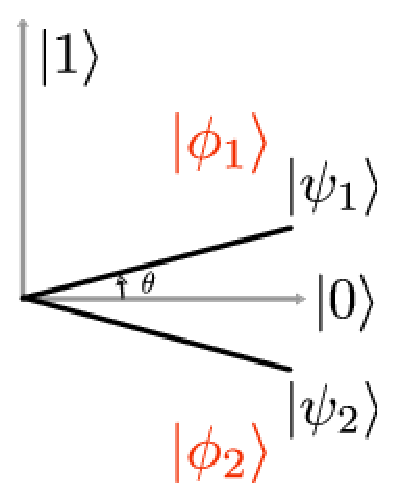
\includegraphics[width=8.5cm,height=8.5cm]{state_separation}
\par\end{centering}

\protect\caption[\hspace{1cm}State separation]{The input states $\left\{ \protect\ket{\psi_{1}},\protect\ket{\psi_{2}}\right\} $
are separated into a pair of more orthogonal states $\left\{ \protect\ket{\phi_{1}},\protect\ket{\phi_{2}}\right\} $
which are more distinguishable.  }


\label{fig:state_separation} 
\end{figure}


%%%%%%%%%%%%%%%%%%%%%%%%%%%%%%%%%%%%%%%%%%%%%%%%
%%%%%%%%%%%%%%%%%%%%%%%%%%%%%%%%%%%%%%%%%%%%%%%%
\section{State Separation: equal priors}

Chefles and Barnett \cite{Chefles1998a} solve the problem of equal
priors employing Kraus representation of quantum maps $\left\{ \hat{A},\hat{A}^{\dagger}\right\} .$
However the solution is more straightforward using the Neumark setup
in (\ref{eq:separation}). When the input states are prepared with
equal priors $\eta_{1}=\eta_{2},$ the solution is directly derived
from the constraint in (\ref{eq:separation constraint}) and no further
optimization is necessary:

\begin{eqnarray}
s & = & ps'+q,\nonumber \\
p & = & \frac{1-s}{1-s'}.\label{eq:separation-1}
\end{eqnarray}


We will now show applications of state separation to exact cloning
and unambiguous state discrimination. Another application to state
separation for equal priors is in hybrid cloning, see Section (3.6.1).
Let us begin by showing the connection to exact cloning with failure
rate. Suppose we are given a quantum system in either of the pure
states $\left\{ \ket{\psi_{1}},\ket{\psi_{2}}\right\} $, such that
the two states are non-orthogonal. The task is to produce two perfect
copies of the input state. Let us embed the quantum system with a
blank state $\ket i$ so the system becomes $\left\{ \ket{\psi_{1}}\ket i,\ket{\psi_{2}}\ket i\right\} $.
A perfect copying machine should produce $\left\{ \ket{\psi_{1}}\ket{\psi_{1}},\ket{\psi_{2}}\ket{\psi_{2}}\right\} $.
A modified Neumark setup from state separation in (\ref{eq:separation})
for cloning is:

\begin{eqnarray}
U|\psi_{1}\rangle|i\rangle & = & \sqrt{p}\ket{\psi_{1}}\ket{\psi_{1}}\ket{\alpha}+\sqrt{q}|\Phi_{o}\rangle|f\rangle,\nonumber \\
U|\psi_{2}\rangle|i\rangle & = & \sqrt{p}\ket{\psi_{1}}\ket{\psi_{1}}\ket{\alpha}+\sqrt{q}|\Phi_{o}\rangle|f\rangle,\label{eq:cloning}
\end{eqnarray}


The inner product gives the unitarity constraint which is enough to
fully solve the problem:

\begin{eqnarray}
s & = & ps^{2}+q\nonumber \\
p & = & \frac{1-s}{1-s^{2}}=\frac{1}{1+s}\label{eq:cloning-1}
\end{eqnarray}


We notice that the success probability of producing two perfect clones
with a rate of abstention (\ref{eq:cloning-1}) could be derived from
state separation success rate in Eq. (\ref{eq:separation-1}) by replacing
the overlap of output states $s'$ with the square overlap of input
states $s^{2}$. This shows that the Duan-Guo limit \cite{Duan1998}
is a special case of state separation. 

More generally, state separation can be modified to produce $N$ copies
of $\left\{ \ket{\psi_{1}},\ket{\psi_{2}}\right\} $ from $M$ initial
copies, where $N\geq M$. We derived the solution of $M$ to $N$
cloning in section (3.2.1). It could simply be derived from Eq. (\ref{eq:separation-1})
replacing the overlap of input states $s$ with $s^{M}$, the overlap
of $M$ states, and $s'$ by $s^{N},$ the overlap of the clones. 

State separation also reproduces the IDP limit in state discrimination
for the case when the states are prepared with arbitrary priors. Simply
setting the overlap of the output states to zero $s'=0$, so that
the states have been separated and are fully distinguishable, produces
the IDP limit $p=1-s$. 

%%%%%%%%%%%%%%%%%%%%%%%%%%%%%%%%%%%%%%%%%%%%%%%%
%%%%%%%%%%%%%%%%%%%%%%%%%%%%%%%%%%%%%%%%%%%%%%%%
\section{State Separation: unequal priors }

We now seek to generalize the results of state separation to the case
when the possible input states $\left\{ \ket{\psi_{1}},\ket{\psi_{2}}\right\} $
are prepared with different a priori probabilities. All the symmetries
enjoyed for equal priors break down and in order to obtain a fully
analytical solution one would have to solve a sixth order equation.
Instead we resort to solving the problem geometrically as the solution
turns out to be more insightful. The Neumark setup is shown in (\ref{eq:separation})
and the constraint in (\ref{eq:separation constraint}). 

We resort to the parametrization of the probabilities giving the curve
$(s,\min s')$ in parametric form, rather than attempting to give
min $s'$ as an explicit function of $s$, which would require solving
a high degree polynomial equation. We choose a change of variables
which linearizes the unitarity constraint (\ref{eq:separation constraint}):
\begin{equation}
p_{1}p_{1}=t^{2},\quad q_{1}q_{2}=z^{2}.\label{eb cha qs -> z =000026 t}
\end{equation}
 The condition becomes 
\begin{equation}
z=s-s't,\qquad0\le t,z\le1,\qquad0\le s'\le s.
\end{equation}
It is a straight line in the first quadrant of the plane $t$-$z$
with negative slope~$-s'$ and crossing the $z$-axis at $z=s$.
From the first equation in ~(\ref{eb cha qs -> z =000026 t}) we
have 
\[
t^{2}=(1-q_{1})(1-q_{2})=1+z^{2}-q_{1}-q_{2}.
\]
Solving for $q_{2}$ and substituting back in the second equation
in ~(\ref{eb cha qs -> z =000026 t}) we have 
\[
q_{1}(q_{1}-1+t^{2}-z^{2})+z^{2}=0.
\]
We now solve for $q_{1}$ and obtain 
\[
q_{1}=\frac{1+z^{2}-t^{2}\pm\sqrt{(1+z^{2}-t^{2})^{2}-4z^{2}}}{2}.
\]
Similarly, for $q_{2}$ we obtain 
\[
q_{2}=\frac{1+z^{2}-t^{2}\mp\sqrt{(1+z^{2}-t^{2})^{2}-4z^{2}}}{2}.
\]
Therefore, the condition $Q=\eta_{1}q_{1}+\eta_{2}q_{2}$ becomes
\[
2Q=1+z^{2}-t^{2}\pm(\eta_{1}-\eta_{2})\sqrt{(1+z^{2}-t^{2})^{2}-4z^{2}}.
\]
We now solve for $z^{2}$. After a bit of algebra we obtain
\begin{eqnarray*}
z^{2} & = & \frac{2\eta_{1}\eta_{2}(1+\tau)-1+Q+\sqrt{\left(1-4\eta_{1}\eta_{2}\right)\left[(1-Q)^{2}-4\eta_{1}\eta_{2}\tau\right]}}{2\eta_{1}\eta_{2}}\\
 & \equiv & \zeta(\tau)
\end{eqnarray*}
where $\tau\equiv t^{2}$. Since $z^{2}$ cannot be less than zero,
we picked up the plus sign for the root. Let us assume that $0\le\eta_{1}\le1/2$
to simplify the analysis. We need to locate the maximum of $z$. For
that, 
\[
\frac{dz}{dt}=\frac{d\sqrt{\zeta}}{d\tau}2t=\frac{d\zeta}{d\tau}\frac{t}{z}.
\]
The derivative $d\zeta/d\tau$ is immediate. We find that the maximum
is located at 
\[
t_{{\rm min}}=\left\{ \begin{array}{lll}
{\displaystyle \sqrt{\left(1-\frac{Q}{2\eta_{1}}\right)\left(1-\frac{Q}{2\eta_{2}}\right)},\quad} & {\rm if} & \quad0\le Q\le2\eta_{1}\\[2em]
0,\quad & {\rm if} & \quad2\eta_{1}<Q\le1.
\end{array}\right.
\]
The corresponding values of $z$ are 
\[
z_{{\rm min}}=\left\{ \begin{array}{lll}
{\displaystyle \frac{Q}{2\sqrt{\eta_{1}\eta_{2}}},\quad} & {\rm if} & \quad0\le Q\le2\eta_{1}\\[2em]
{\displaystyle \sqrt{\frac{Q-\eta_{1}}{\eta_{2}}},\quad} & {\rm if} & \quad2\eta_{1}<Q\le1.
\end{array}\right.
\]
There is a second point that we need to define. We first note that
for equal priors the curve is simply the hyperbola 
\[
z^{2}=t^{2}+2Q-1,
\]
which intersects the straight line 
\[
z=1-t
\]
at the point 
\[
\left(z,t\right)=\left(Q,1-Q\right).
\]
By trying this solution in $z^{2}=\zeta(t^{2})$ we note that it is
actually a general solution for any $\eta_{1}$, $\eta_{2}$. Moreover,
the straight line $z=1-t$ is tangent to~$z^{2}=\zeta(t^{2})$ at
$(Q,1-Q)$ for any values of $\eta_{1}$, $\eta_{2}$, as can be checked
by substituting in the formula $dz/dt=(t/z)(d\zeta/d\tau)$. Note
also that $z=1-t$ is the limiting line for the family $z=s-s't$.
Hence, an obvious parametrization for the curve $(s,s')$ is obtained
as follows: {\em i}.~define 
\[
s'(t)=-\frac{dz}{dt}=-\frac{t\,\zeta'(t^{2})}{\sqrt{\zeta(t^{2})}},\qquad t_{{\rm min}}\le t\le1-Q,
\]
and next {\em ii}.~define 
\[
s(t)=z+ts'(t)=\sqrt{\zeta(t^{2})}+ts'(t),\qquad t_{{\rm min}}\le t\le1-Q,
\]
where 
\[
\zeta'(\tau)=1-\frac{\sqrt{1-4\eta_{1}\eta_{2}}}{\sqrt{(1-Q)^{2}-4\eta_{1}\eta_{2}\tau}}.
\]


For $s<z_{{\rm min}}$ it is always possible to separate the initial
states, i.e., $|\psi_{1}\rangle$ and~$|\psi_{2}\rangle$ can be
made orthogonal. We note that the condition $s=z_{{\rm min}}$ is
equivalent to the unambiguous discrimination result 
\[
Q=2\sqrt{\eta_{1}\eta_{2}}s,\quad Q=\eta_{1}+\eta_{2}s^{2}.
\]


\begin{figure}
\includegraphics[width=8.5cm,height=8.5cm]{Separation1\lyxdot graph}

\protect\caption[\hspace{1cm}$s'$ vs. $s$]{The plot is for $\eta_{1}=0.1$. As $\eta_{1}$ approaches $1/2$
the curves approach a straight line. The difference is more noticeable
for very small values of $\eta_{1}$.}


\label{s' vs s}
\end{figure}

%%%%%%%%%%%%%%%%%%%%%%%%%%%%%%%%%%%%%%%%%%%%%%%%
%%%%%%%%%%%%%%%%%%%%%%%%%%%%%%%%%%%%%%%%%%%%%%%%
\chapter{Linear Optical Experimental Realizations}

Choosing a physical system to realize quantum information processes,
which have otherwise been solved theoretically, is central challenge
to building a quantum computer. Some of the systems in use today are:
energy levels of ions, the orientation of nuclear spin, the presence
or absence of a photon in a cavity \cite{Cirac1995,Gershenfeld1997,Turchette1995,Domokos1995}
and dual rail representation of a qubit proposed by Milburn \cite{Milburn1989}
and later by Chuang and Yamamoto \cite{Chuang1996}. We will realize
the implementation of our works using the dual rail representation
of photons combined with a six-port, which is a linear device with
three input and three output ports. The six-port can be realized with
beamsplitters and phase shifters. First we will demonstrate the power
and simplicity of this system by working out the implementation of
UD following the work by Bergou $et$ $al.$ \cite{Bergou2009}. 

In our work \cite{shehu} we generalized the optical implementation
schemes to state discrimination which optimally interpolates between
UD and ME with a fixed rate of inconclusive results FRIO. Ever since
the interpolation scheme of a general measurement with FRIO was derived
by Bagan $et$ $al$ \cite{Bagan2012} there has been a quest for
a physical realization. The authors solved the problem using an operator
transformation technique that reformulated the intermediate problem
into a ME problem with an extra optimization parameter. Essentially
they reduced the problem from a three element POVM to two element
POVM similar to ME. Inspired by the work of Reck and Zeilinger \cite{Reck1994}
in which they prove that any discreet finite dimensional unitary operator
can be constructed in the lab as a multi-port interferometer using
beamsplitters and phase shifters we set out to solve the FRIO using
the Neumark setup as it lends itself into an optical implementation.
This gives us a closed form solution as in Bagan $et$ $al.$ In addition
it gives a three dimensional unitary operator where all the coefficients
are explicitly calculated in terms of a priori probabilities, overlap
of the input states and FRIO. Using the Reck $et$ $al.$ algorithm
the unitary is decomposed in terms of beam splitters with corresponding
coefficients of transmittance and reflectivity. The setup reduces
into the UD by setting the error rate to zero, in turn it reproduces
the work of Bergou $et\hspace{0.3cm}al$ \cite{Bergou2009}. At the
other extreme it produces the setup to ME for FRIO equal to zero. 

%%%%%%%%%%%%%%%%%%%%%%%%%%%%%%%%%%%%%%%%%%%%%%%%
%%%%%%%%%%%%%%%%%%%%%%%%%%%%%%%%%%%%%%%%%%%%%%%%




An immediate application is that it can now
be used in the calculations of the coefficients beam splitters. 
%%%%%%%%%%%%%%%%%%%%%%%%%%%%%%%%%%%%%%%%%%%%%%%%
%%%%%%%%%%%%%%%%%%%%%%%%%%%%%%%%%%%%%%%%%%%%%%%%
\section{Choosing the physical implementation }

The main reason to seek a solution using the Neumark setup is because
it lends itself to an optical implementation. This implementation,
as we will see, can be carried out using only linear optical elements
(beam splitters and a mirror). The possible states are represented
by single photons and a photodetector will carry out the measurement
process at the output. To choose the basis we start with the two mode
vacuum state $|00\rangle.$ The total number of photons in both modes
is one. This two dimensional Hilbert space where our photons live
can be spanned by the states $\{|10\rangle,|01\rangle\}$, where $|10\rangle=a_{1}^{\dagger}|00\rangle$
and $|01\rangle=a_{2}^{\dagger}|00\rangle$ and $a_{i}^{\dagger}$
are creation operators corresponding to two different modes of the
electromagnetic field. The basis $\{|10\rangle,|01\rangle\}$ corresponds
to the basis of qubit in $\{|0\rangle,|1\rangle\}.$ The most general
input state can be written as $|\psi_{i}\rangle=\alpha_{i}|0\rangle+\beta_{i}|1\rangle=\alpha_{i}|10\rangle+\beta_{i}|01\rangle$
which can be produced by sending a photon into a beam splitter with
some transmission and reflection coefficient, where the modes 1 and
2 correspond to the output modes of the beam splitter. 

A general $2N$ port is a linear device with $N$ input and $N$ output
ports. It can be constructed from beam splitters and mirrors \cite{Bergou2009}.
For our work we will need a six-port, three input ports and three
output ports. Let us denote the annihilation operators corresponding
to the input modes by $a_{j\text{\thinspace in }},$ $j=1,2,3$ then
the output operators are given by

\[
a_{j\text{\thinspace out }}=U^{-1}a_{i\text{\thinspace in }}U=\sum M_{jk}a_{k\text{\thinspace in }},
\]
where $M_{jk}$ are the elements of the $N\times N$ unitary matrix
$M.$ In the Schrodinger picture, the $in$ and $out$ states are
related by 

\[
\ket{\psi}_{out}=U\ket{\psi}_{in}.
\]
 In general an $in$ state that contains a single photon can be described
by

\[
\ket{\psi}_{in}=\sum_{j=1}^{3}c_{j}a_{j}^{\dagger}\ket{000},
\]
 where $\sum_{j=1}^{3}\left|c_{j}\right|=1.$ The output state is
given by

\begin{eqnarray*}
\ket{\psi}_{in} & = & U\sum_{j=1}^{3}c_{j}a_{j}^{\dagger}U^{-1}\ket{000}\\
 & = & \sum_{j,k=1}^{3}c_{j}M_{jk}^{T}a_{j}^{\dagger}\ket{000},
\end{eqnarray*}
where we have made use of the fact that the vacuum is invariant under
the transformation, $U$. To simplify the notation in the implementation
section let:$\ket{100}\equiv\ket 1,\thinspace\ket{010}\equiv\ket 2,\thinspace\ket{001}\equiv\ket 3.$ 

%%%%%%%%%%%%%%%%%%%%%%%%%%%%%%%%%%%%%%%%%%%%%%%%
%%%%%%%%%%%%%%%%%%%%%%%%%%%%%%%%%%%%%%%%%%%%%%%%
\section{Implementation: equal priors}

We will first show the implementation of FRIO for equal priors. The
Neumark in direct sum notation setup will be used to calculate the
unitary matrix. The two input states to be discriminated can be written
as $|\psi_{1}\rangle_{in}=|1\rangle$ and $|\psi_{2}\rangle_{in}=\cos\theta|1\rangle+\sin\theta|2\rangle$. 

\begin{eqnarray}
U|1\rangle & = & \sqrt{p}|1\rangle+\sqrt{r}|2\rangle+\sqrt{q}|3\rangle,\label{eq:eq1}\\
U(\cos\theta|1\rangle+\sin\theta|2\rangle) & = & \sqrt{r}|1\rangle+\sqrt{p}|2\rangle+\sqrt{q}|3\rangle,\label{eq:eq2}
\end{eqnarray}
where the error and success rate was calculated in section 4.1.1:
\begin{eqnarray}
r & = & \frac{1}{2}\left[(1-Q)-\sqrt{(1-Q)^{2}-(Q_{o}-Q)^{2}}\right],\label{eq:r}\\
p & = & \frac{1}{2}\left[(1-Q)+\sqrt{(1-Q)^{2}-(Q_{o}-Q)^{2}}\right],\label{eq:p}
\end{eqnarray}


From the Neumark setup we can read out six out of nine elements of
the unitary matrix. Eq. (\ref{eq:eq1}) gives the first column, Eq.
(\ref{eq:eq2}) gives the second column and the last column can be
constructed from the conditions of unitarity. 

To get first column, multiply Eq. (\ref{eq:eq1}) from the left with
$\bra 1,$ $\bra 2$ and $\bra 3:$

\[
\langle1|U|1\rangle=U_{11}=\sqrt{p},
\]
 

\[
\langle2|U|1\rangle=U_{21}=\sqrt{q},
\]


\[
\langle3|U|1\rangle=U_{31}=\sqrt{r}.
\]
To get the second column, multiply \ref{eq:eq2} from the left with
$\bra 1,$ $\bra 2$ and $\bra 3:$

\[
\cos\theta\langle1|U|1\rangle+\sin\theta\langle1|U|2\rangle=\cos\theta U_{11}+\sin\theta U_{12}=\sqrt{r},
\]


\[
\cos\theta\langle2|U|1\rangle+\sin\theta\langle2|U|2\rangle=\cos\theta U_{21}+\sin\theta U_{22}=\sqrt{p},
\]


\[
\cos\theta\langle3|U|1\rangle+\sin\theta\langle3|U|2\rangle=\cos\theta U_{31}+\sin\theta U_{32}=\sqrt{q}.
\]
 Using the solution of the first column $U_{i1}$, gives the entries
to second column $U_{i2}$ ($i=1,2,3),$ 

$\cos\theta\sqrt{p}_{1}+\sin\theta U_{12}=\sqrt{r_{2}}\Rightarrow$
$U_{12}=\frac{\sqrt{r}-\sqrt{p}Q_{o}}{\sqrt{1-Q_{o}^{2}}}$,

$\cos\theta\sqrt{q_{1}}+\sin\theta U_{22}=\sqrt{p_{2}}\Rightarrow$
$U_{22}=\frac{[\sqrt{p}-\sqrt{r}Q_{o}]}{\sqrt{1-Q_{o}^{2}}}$,

$\cos\theta\sqrt{r_{1}}+\sin\theta U_{32}=\sqrt{q_{2}}\Rightarrow$
$U_{32}=\sqrt{\frac{Q(1-Q_{o})}{1+Q_{o}}}$ ,

where $\cos\theta=Q_{o}$ and $\sin\theta=\sqrt{1-Q_{o}^{2}}$

The remaining elements be calculated from the conditions of the unitarity,
$U^{T}U=I$, $U_{i1}^{2}+U_{i2}^{2}+U_{i3}^{2}=1$ where $i=1,2,3$

$U_{13}=\pm\sqrt{1-U_{11}^{2}-U_{12}^{2}}=\pm\sqrt{1-p-\frac{r+pQ_{o}^{2}-2\sqrt{pr}Q_{0}}{1-Q_{0}^{2}}}=\pm\sqrt{\frac{Q-Q_{o}^{2}+2\sqrt{pr}Q_{0}}{1-Q_{0}^{2}}}=\pm\sqrt{\frac{Q}{1-Q_{0}}}$, 

the relation $\sqrt{pr}=\frac{1}{2}(Q_{o}-Q)$ was used, which is
derived from the multiplication of (\ref{eq:r}) and (\ref{eq:p}). 

$U_{23}=\pm\sqrt{1-U_{21}^{2}-U_{22}^{2}}=\pm\sqrt{1-r-\frac{p+rQ_{o}^{2}-2\sqrt{pr}Q_{0}}{1-Q_{0}^{2}}}=\pm\sqrt{\frac{Q}{1-Q_{0}}}$,

$U_{33}=\pm\sqrt{1-U_{31}^{2}-U_{32}^{2}}=\pm\sqrt{1-Q-\frac{Q(1-Q_{o})}{1+Q_{o}}}=\pm\sqrt{\frac{1+Q_{o}-2Q}{1+Q_{o}}}=\pm\frac{\sqrt{p}+\sqrt{r}}{\sqrt{1+Q_{o}}}$.

It is important to notice the relation $\sqrt{(1+Q_{o}-2Q)}=\sqrt{p}+\sqrt{r}$
which is somewhat unexpected. 

The full unitary, with the signs of the last column elements chosen
so that $U_{13}^{2}+U_{23}^{2}+U_{33}^{2}=1,$ is

\begin{equation}
U=\begin{pmatrix}\sqrt{p} & \frac{\sqrt{r}-\sqrt{p}Q_{o}}{\sqrt{1-Q_{o}^{2}}} & -\sqrt{\frac{Q}{1+Q_{o}}}\\
\sqrt{r} & \frac{\sqrt{p}-\sqrt{r}Q_{o}}{\sqrt{1-Q_{o}^{2}}} & -\sqrt{\frac{Q}{1+Q_{o}}}\\
\sqrt{Q} & \sqrt{\frac{Q(1-Q_{o})}{1+Q_{o}}} & \frac{\sqrt{p}+\sqrt{r}}{\sqrt{1+Q_{o}}}
\end{pmatrix}.\label{eq:U(equal prior)}
\end{equation}
In this representation the above matrix can be shown that it satisfies
all the unitary conditions. 

The unitary in (\ref{eq:U(equal prior)}) interpolates between the
optimal ME and UD schemes varying the fixed rate of inconclusive results
$Q.$ Setting the failure rate to zero, $Q=0,$ collapses it into
the unitary of optimal ME:

\[
U_{ME}=\begin{pmatrix}\sqrt{p} & \frac{\sqrt{r}-\sqrt{p}Q_{o}}{\sqrt{1-Q_{o}^{2}}} & 0\\
\sqrt{r} & \frac{\sqrt{p}-\sqrt{r}Q_{o}}{\sqrt{1-Q_{o}^{2}}} & 0\\
0 & 0 & 1
\end{pmatrix},
\]
which can be simplified further by noticing $(U_{12})^{2}=\left(\frac{\sqrt{r}-\sqrt{p}Q_{o}}{\sqrt{1-Q_{o}^{2}}}\right)^{2}=r,$
similarly $(U_{22})^{2}=\left(\frac{\sqrt{p}-\sqrt{r}Q_{o}}{\sqrt{1-Q_{o}^{2}}}\right)^{2}=p$,
simplifying the unitary into: 

\[
U_{ME}=\begin{pmatrix}\sqrt{p} & \sqrt{r} & 0\\
\sqrt{r} & -\sqrt{p} & 0\\
0 & 0 & 1
\end{pmatrix},
\]
only one beam splitter in needed for optimal ME measurements. 

On the other hand setting the error rate of the unitary \ref{eq:U(equal prior)}
to zero gives the optimal UD unitary,

\[
U_{UD}=\begin{pmatrix}\sqrt{p} & -\frac{\sqrt{p}Q_{o}}{\sqrt{1-Q_{o}^{2}}} & -\sqrt{\frac{Q_{0}}{1+Q_{o}}}\\
0 & \frac{\sqrt{p}}{\sqrt{1-Q_{o}^{2}}} & -\sqrt{\frac{Q_{o}}{1+Q_{o}}}\\
\sqrt{Q_{0}} & \sqrt{\frac{Q_{o}(1-Q_{o})}{1+Q_{o}}} & \sqrt{\frac{1-Q_{o}}{1+Q_{o}}}
\end{pmatrix}.
\]


All three beamsplitters are still necessary for a general UD measurement.
This is because the measurement is essentially two-step: in the first
step the states are made orthogonal, then upon succeeding a projective
measurement is performed. 

Let us now express the interpolating unitary in terms of three beamsplitters,
as $U=M_{1}M_{2}M_{3}$. This ordering was derived using the Reck-Zeilinger
algorithm which says that any discreet finite unitary matrix can be
expressed in terms of beamsplitters and phase shifters. The beamsplitters
can be written in terms of $\sin\omega_{i}$ and $\cos\omega_{i}$
and it is easy to check the unitarity condition, $\sin^{2}\omega_{i}+\cos^{2}\omega_{i}=1.$
Then the task is that of calculating $\omega_{i}.$

\[
M_{1}=\begin{pmatrix}\sin\omega & \cos\omega_{1} & 0\\
\cos\omega & -\sin\omega & 0\\
0 & 0 & 1
\end{pmatrix},
\]


\[
M_{2}=\begin{pmatrix}\sin\omega_{2} & 0 & \cos\omega_{2}\\
0 & 1 & 0\\
\cos\omega_{2} & 0 & -\sin\omega_{2}
\end{pmatrix},
\]


\[
M_{3}=\begin{pmatrix}1 & 0 & 0\\
0 & \sin\omega_{3} & \cos\omega_{3}\\
0 & \cos\omega_{3} & -\sin\omega_{3}
\end{pmatrix},
\]


\[
U=M_{1}M_{2}M_{3}=\begin{pmatrix}\sqrt{p} & \frac{\sqrt{r}-\sqrt{p}Q_{o}}{\sqrt{1-Q_{o}^{2}}} & \sqrt{\frac{Q}{1+Q_{o}}}\\
\sqrt{r} & \frac{[\sqrt{p}-\sqrt{r}Q_{o}]}{\sqrt{1-Q_{o}^{2}}} & \sqrt{\frac{Q}{1+Q_{o}}}\\
\sqrt{Q} & \sqrt{\frac{Q(1-Q_{o})}{1+Q_{o}}} & \sqrt{\frac{1+Q_{o}-2Q}{1+Q_{o}}}
\end{pmatrix}
\]


\[
=\begin{pmatrix}\sin\omega_{1}\sin\omega_{2} & \cos\omega_{1}\sin\omega_{3}+\sin\omega_{1}\cos\omega_{2}\cos\omega_{3} & \cos\omega_{1}\cos\omega_{3}-\sin\omega_{1}\cos\omega_{2}\sin\omega_{3}\\
\cos\omega_{1}\sin\omega_{2} & -\sin\omega_{1}\sin\omega_{3}+\cos\omega_{1}\cos\omega_{2}\cos\omega_{3} & -\sin\omega_{1}\cos\omega_{3}-\cos\omega_{1}\cos\omega_{2}\sin\omega_{3}\\
\cos\omega_{2} & -\sin\omega_{2}\cos\omega_{3} & \sin\omega_{2}\sin\omega_{3}
\end{pmatrix}.
\]


This gives nine equations and only three independent variables to
be calculated. All the elements can be obtained by using just $U_{31},U_{32},U_{21}:$ 

$\cos\omega_{2}=U_{31}=\sqrt{Q},\sin\omega_{2}=\sqrt{1-r^{2}}=\sqrt{1-Q}$, 

$\cos\omega_{3}=-\sqrt{\frac{Q(1-Q_{o})}{(1+Q_{o})(1-Q)}},\sin\omega_{3}=\sqrt{\frac{1+Q_{o}-2Q}{(1-Q)(1+Q_{o})}}=\frac{\sqrt{p}+\sqrt{r}}{\sqrt{(1-Q)(1+Q_{o})}}$, 

$\cos\omega_{1}=\sqrt{\frac{r}{1-Q}},\sin\omega_{1}=\sqrt{\frac{p}{1-Q}}$. 

The three beamsplitters with the proper coefficients of reflectivity
and transmittance are:

\[
M_{1}=\begin{pmatrix}\sqrt{\frac{p}{1-Q}} & \sqrt{\frac{r}{1-Q}} & 0\\
\sqrt{\frac{r}{1-Q}} & -\sqrt{\frac{p}{1-Q}} & 0\\
0 & 0 & 1
\end{pmatrix},
\]


\[
M_{2}=\begin{pmatrix}\sqrt{1-Q} & 0 & \sqrt{Q}\\
0 & 1 & 0\\
\sqrt{Q} & 0 & -\sqrt{1-Q}
\end{pmatrix},
\]


\[
M_{3}=\begin{pmatrix}1 & 0 & 0\\
0 & \sqrt{\frac{1+Q_{o}-2Q}{(1-Q)(1+Q_{o})}} & -\sqrt{\frac{Q(1-Q_{o})}{(1+Q_{o})(1-Q)}}\\
0 & -\sqrt{\frac{Q(1-Q_{o})}{(1+Q_{o})(1-Q)}} & -\sqrt{\frac{1+Q_{o}-2Q}{(1-Q)(1+Q_{o})}}
\end{pmatrix},
\]


\bigskip{}


By choosing the FRIO this matrix minimizes the error rate and maximizes
the rate of success. Hence, by setting the FRIO to zero we obtain
the setup to the minimum error problem. On the other hand, setting
the error rate to zero gives the setup of the optimal unambiguous
discrimination where the optimal inconclusive rate is the $Q_{o}=s$.
This simplifies the works of the experimentalists because now they
only need one setup and are not restrained to the extreme points.

%%%%%%%%%%%%%%%%%%%%%%%%%%%%%%%%%%%%%%%%%%%%%%%%
%%%%%%%%%%%%%%%%%%%%%%%%%%%%%%%%%%%%%%%%%%%%%%%%
\section{Implementation: Unequal priors}

In this section we derive the beamsplitter coefficients necessary
to interpolate minimum error measurements with a $FRIO$ when the
input states are prepared with different a priori probabilities. The
two input states to be discriminated are $|\psi_{1}\rangle_{in}=|1\rangle$
and $|\psi_{2}\rangle_{in}=\cos\theta|1\rangle+\sin\theta|2\rangle$.
A unitary operator carries out the operation:

\begin{align}
U|1\rangle & =\sqrt{p_{1}}|1\rangle+\sqrt{r_{1}}|2\rangle+\sqrt{q_{1}}|3\rangle,\label{eq:U1}\\
U(\cos\theta|1\rangle+\sin\theta|2\rangle) & =\sqrt{r_{2}}|1\rangle+\sqrt{p_{2}}|2\rangle+\sqrt{q_{2}}|3\rangle.\label{eq:U2}
\end{align}


The error and success rates where calculated in Section 4.1.4

\begin{align}
r_{i} & =\frac{1}{2}\left[(1-\frac{Q}{2\eta_{i}})-\frac{(1-\frac{Q}{2\eta_{i}})(1-Q)-\frac{1}{2\eta_{i}}(Q_{o}-Q)^{2}}{\sqrt{(1-Q)^{2}-(Q-Q_{o})^{2}}}\right],\\
p_{i} & =\frac{1}{2}\left[(1-\frac{Q}{2\eta_{i}})+\frac{(1-\frac{Q}{2\eta_{i}})(1-Q)-\frac{1}{2\eta_{i}}(Q_{o}-Q)^{2}}{\sqrt{(1-Q)^{2}-(Q-Q_{o})^{2}}}\right].
\end{align}


From the two equation in (\ref{eq:U1}) and (\ref{eq:U2}) we can
read out six of nine elements of the three by three unitary matrix.
Multiplying (\ref{eq:U1}) on the left hand side by $\{\langle1|,\bra 2,\bra 3\}$
will give the elements $U_{i1},$ $i=1,2,3.$ Similarly we can obtain
three more elements for the second column. 

The first column is:

$\langle1|U|1\rangle=U_{11}=\sqrt{p_{1}},$

$\langle2|U|1\rangle=U_{21}=\sqrt{q_{1}},$

$\langle3|U|1\rangle=U_{31}=\sqrt{r_{1}}.$

Second Column:

$\cos\theta\langle1|U|1\rangle+\sin\theta\langle1|U|2\rangle=\cos\theta U_{11}+\sin\theta U_{12}=\sqrt{r_{2}},$

$\cos\theta\langle2|U|1\rangle+\sin\theta\langle2|U|2\rangle=\cos\theta U_{21}+\sin\theta U_{22}=\sqrt{p_{2}},$

$\cos\theta\langle3|U|1\rangle+\sin\theta\langle3|U|2\rangle=\cos\theta U_{31}+\sin\theta U_{32}=\sqrt{q_{2}}$
.

Using the solution of the first column $U_{i1}$, gives the explicit
entries to second column $U_{i2}:$ 

$\cos\theta\sqrt{p}_{1}+\sin\theta U_{12}=\sqrt{r_{2}}\Rightarrow$
$U_{12}=\frac{\sqrt{r_{2}}-\sqrt{p_{1}}\cos\theta}{\sin\theta}$,

$\cos\theta\sqrt{q_{1}}+\sin\theta U_{22}=\sqrt{p_{2}}\Rightarrow$
$U_{22}=\frac{\sqrt{p_{2}}-\sqrt{r_{1}}\cos\theta}{\sin\theta}$,

$\cos\theta\sqrt{r_{1}}+\sin\theta U_{32}=\sqrt{q_{2}}\Rightarrow$
$U_{32}=\frac{\sqrt{q_{2}}-\sqrt{q_{1}}\cos\theta}{\sin\theta}$,

The last column be calculated from the conditions of the unitarity,
$U^{T}U=I$, $U_{i1}^{2}+U_{i2}^{2}+U_{i3}^{2}=1$ where $i=1,2,3$

$U_{13}=\pm\sqrt{1-U_{11}^{2}-U_{12}^{2}}=\pm\sqrt{1-p_{1}-\frac{r_{2}+p_{1}\cos\theta-2\sqrt{p_{1}r_{2}}\cos\theta}{\sin^{2}\theta}}=\pm\frac{\sqrt{\sin^{2}\theta-p_{1}-r_{2}+2\sqrt{p_{1}r_{2}}\cos\theta}}{\sin\theta}$.

Similarly:

$U_{23}=\pm\frac{\sqrt{\sin^{2}\theta-r_{1}-p_{2}+2\sqrt{p_{2}r_{1}}\cos\theta}}{\sin\theta},$

$U_{33}=\pm\frac{\sqrt{sin^{2}\theta-q_{1}-q_{2}+2\sqrt{q_{1}q_{2}}\cos\theta}}{\sin\theta}.$

Now that all the elements have been calculated the unitary is: 

\begin{equation}
U=\begin{pmatrix}\sqrt{p_{1}} & \frac{\sqrt{r_{2}}-\sqrt{p_{1}}\cos\theta}{\sin\theta} & -\frac{\sqrt{\sin^{2}\theta-p_{1}-r_{2}+2\sqrt{p_{1}r_{2}}\cos\theta}}{\sin\theta}\\
\sqrt{r_{1}} & \frac{\sqrt{p_{2}}-\sqrt{r_{1}}\cos\theta}{\sin\theta} & -\frac{\sqrt{\sin^{2}\theta-r_{1}-p_{2}+2\sqrt{p_{2}r_{1}}\cos\theta}}{\sin\theta}\\
\sqrt{q_{1}} & \frac{\sqrt{q_{2}}-\sqrt{q_{1}}\cos\theta}{\sin\theta} & +\frac{\sqrt{sin^{2}\theta-q_{1}-q_{2}+2\sqrt{q_{1}q_{2}}\cos\theta}}{\sin\theta}
\end{pmatrix}.
\end{equation}


\smallskip{}


It is worth mentioning that all equations in this section referencing
$r_{i}$ and $p_{i}$ are using the optimal values (\ref{eq:r_i})
and (\ref{eq:p_i}) derived in the previous section.

Now that we have a full unitary matrix we want to express it in terms
of linear optical devices. Again the Reck-Zeilinger algorithm is used
to decompose the unitary in terms of beamsplitters and their ordering
\ref{sixport}. The operator $U$ is decomposed into beamsplitters
in the order of $U=M_{1}\cdot M_{2}\cdot M_{3}$, and no phase shifters
are needed: 
\begin{align*}
M_{1} & =\begin{pmatrix}\sin\omega_{1} & \cos\omega_{1} & 0\\
\cos\omega_{1} & -\sin\omega_{1} & 0\\
0 & 0 & 1
\end{pmatrix},\\
M_{2} & =\begin{pmatrix}\sin\omega_{2} & 0 & \cos\omega_{2}\\
0 & 1 & 0\\
\cos\omega_{2} & 0 & -\sin\omega_{2}
\end{pmatrix},\\
M_{3} & =\begin{pmatrix}1 & 0 & 0\\
0 & \sin\omega_{3} & \cos\omega_{3}\\
0 & \cos\omega_{3} & -\sin\omega_{3}
\end{pmatrix},\\
\end{align*}


\bigskip{}


\begin{figure}
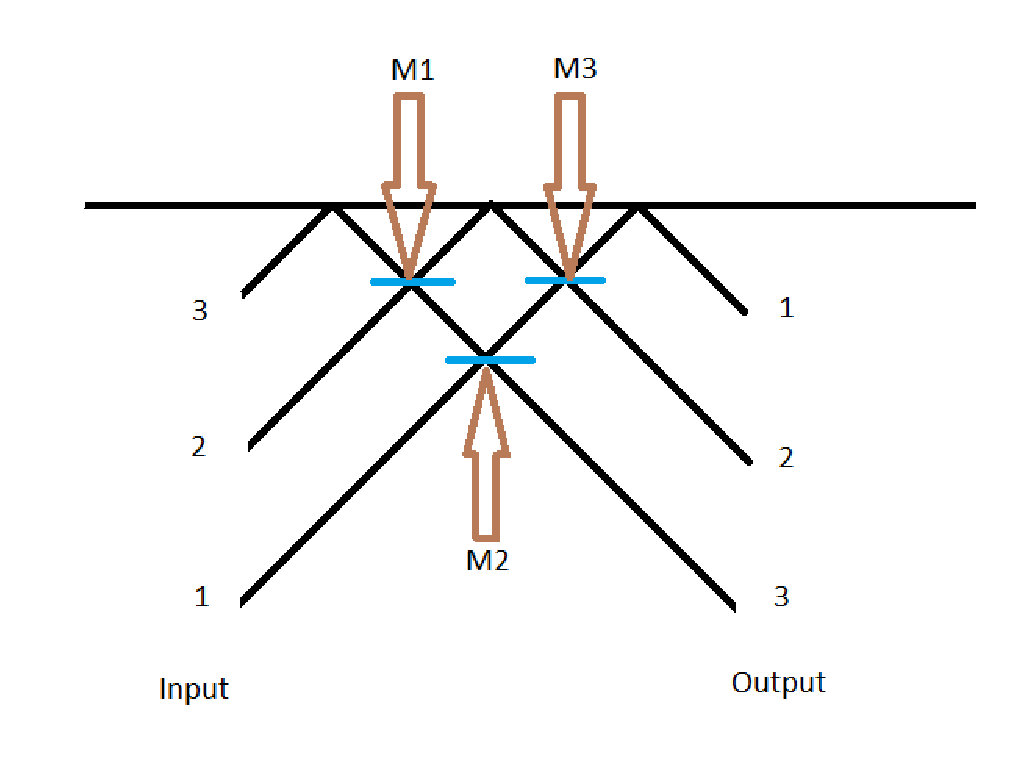
\includegraphics[width=8.5cm,height=8.5cm]{BeamSplitters}

\protect\caption[\hspace{1cm}Six port interferometer]{}


\label{sixport}
\end{figure}
where the coefficients of reflectivity and transmittance are given
by $\sqrt{R_{i}}=\sin\omega_{i}$ and $\sqrt{T_{i}}=\cos\omega_{i}$.

$U=M_{1}M_{2}M_{3}$=$\begin{pmatrix}\sqrt{p_{1}} & \frac{\sqrt{r_{2}}-\sqrt{p_{1}}cos\theta}{sin\theta} & \pm\frac{\sqrt{sin^{2}\theta-p_{1}-r_{2}+2\sqrt{p_{1}r_{2}}cos\theta}}{sin^{2}\theta}\\
\sqrt{r_{1}} & \frac{\sqrt{p_{2}}-\sqrt{r_{1}}cos\theta}{sin\theta} & \pm\frac{\sqrt{sin^{2}\theta-r_{1}-p_{2}+2\sqrt{p_{2}r_{1}}cos\theta}}{sin^{2}\theta}\\
\sqrt{q_{1}} & \frac{\sqrt{q_{2}}-\sqrt{q_{1}}cos\theta}{sin\theta} & \pm\frac{\sqrt{sin^{2}\theta-q_{1}-q_{2}+2\sqrt{q_{1}q_{2}}cos\theta}}{sin^{2}\theta}
\end{pmatrix}$ 

$=\begin{pmatrix}sin\omega_{1}sin\omega_{2} & cos\omega_{1}sin\omega_{3}+sin\omega_{1}cos\omega_{2}cos\omega_{3} & cos\omega_{1}cos\omega_{3}-sin\omega_{1}cos\omega_{2}sin\omega_{3}\\
cos\omega_{1}sin\omega_{2} & -sin\omega_{1}sin\omega_{3}+cos\omega_{1}cos\omega_{2}cos\omega_{3} & -sin\omega_{1}cos\omega_{3}-cos\omega_{1}cos\omega_{2}sin\omega_{3}\\
cos\omega_{2} & -sin\omega_{2}cos\omega_{3} & sin\omega_{2}sin\omega_{3}
\end{pmatrix}$ 

\bigskip{}


The coefficients of reflectivity and transmittance can be calculated
by matching the corresponding elements of the unitary and it's decomposition.
We can get all the elements by using just $U_{31},U_{32}$ and $U_{33}.$

$U_{31}=\sqrt{q_{1}}=\cos\omega_{2},\sin\omega_{2}=\sqrt{1-\cos\omega_{2}^{2}}=\sqrt{1-q_{1}}$, 

$U_{32}=\frac{\sqrt{q_{2}}-\sqrt{q_{1}}cos\theta}{sin\theta}=-\sin\omega_{2}\cos\omega_{3}=-\sqrt{1-q_{1}}\cos\omega_{3}\Rightarrow$
$\cos\omega_{3}=-\frac{1}{\sqrt{1-q_{1}}}[\frac{\sqrt{q_{2}}-\sqrt{q_{1}}cos\theta}{sin\theta}],$

$\sin\omega_{3}=\sqrt{1-\cos\omega_{3}}=-\frac{\sqrt{sin^{2}\theta-q_{1}-q_{2}+2\sqrt{q_{1}q_{2}}cos\theta}}{\sqrt{1-q_{1}}sin\theta},$

$U_{21}=\sqrt{r_{1}}=\cos\omega_{1}\sin\omega_{2}=\cos\omega_{1}\sqrt{1-q_{1}}\Rightarrow$
$\cos\omega_{1}=\sqrt{\frac{r_{1}}{1-q_{1}}},$

$\sin\omega_{1}=\sqrt{1-\cos\omega_{1}}=\sqrt{\frac{p_{1}}{1-q_{1}}}$. 

Substituting the coefficients of reflectivity and transmittance the
beamsplitters are:

$M_{1}=\begin{pmatrix}\sqrt{\frac{p_{1}}{1-q_{1}}} & \sqrt{\frac{r_{1}}{1-q_{1}}} & 0\\
\sqrt{\frac{r_{1}}{1-q_{1}}} & -\sqrt{\frac{p_{1}}{1-q_{1}}} & 0\\
0 & 0 & 1
\end{pmatrix},\,M_{2}=\begin{pmatrix}\sqrt{1-q_{1}} & 0 & \sqrt{q_{1}}\\
0 & 1 & 0\\
\sqrt{q_{1}} & 0 & -\sqrt{1-q_{1}}
\end{pmatrix},$

$M_{3}=\begin{pmatrix}1 & 0 & 0\\
0 & \frac{\sqrt{sin^{2}\theta-q_{1}-q_{2}+2\sqrt{q_{1}q_{2}}cos\theta}}{\sqrt{1-q_{1}}sin\theta} & -\frac{1}{\sqrt{1-q_{1}}}[\frac{\sqrt{q_{2}}-\sqrt{q_{1}}cos\theta}{sin\theta}]\\
0 & -\frac{1}{\sqrt{1-q_{1}}}[\frac{\sqrt{q_{2}}-\sqrt{q_{1}}cos\theta}{sin\theta}] & -\frac{\sqrt{sin^{2}\theta-q_{1}-q_{2}+2\sqrt{q_{1}q_{2}}cos\theta}}{\sqrt{1-q_{1}}sin\theta}
\end{pmatrix}$.

\bigskip{}


All the coefficients can be expressed in terms of the $FRIO$. Using
the optimal relationship between the individual failure rates $\eta_{1}q_{1}=\eta_{2}q_{2}=Q/2$,$\thinspace q_{1}=Q/2\eta_{1},\thinspace q_{2}=Q/2\eta_{2}$
and the above expressions of success and error rates. 

$\cos\omega_{1}=\sqrt{\frac{r_{1}}{1-Q/2\eta_{1}}}$ , $\sin\omega_{1}=\sqrt{\frac{p_{1}}{1-Q/2\eta_{1}}},$

$\cos\omega_{2}=\sqrt{Q/2\eta_{1}}$, $\sin\omega_{2}=\sqrt{1-Q/2\eta_{1}},$

$\cos\omega_{3}=-\frac{\sqrt{Q/2\eta_{2}}-Q_{o}/2\eta_{1}\sqrt{Q/2\eta_{2}}}{\sqrt{(1-Q/2\eta_{1})(1-Q_{o}^{2}/4\eta_{1}\eta_{2})}}$, 

$\sin\omega_{3}=\frac{\sqrt{1-Q_{o}^{2}/4\eta_{1}\eta_{2}-Q/(2\eta_{1}\eta_{2})+QQ_{o}/(2\eta_{1}\eta_{2})}}{\sqrt{(1-Q/2\eta_{1})(1-Q_{o}^{2}/4\eta_{1}\eta_{2})}},$

\bigskip{}


\[
M_{1}=\begin{pmatrix}\sqrt{\frac{p_{1}}{1-Q/2\eta_{1}}} & \sqrt{\frac{r_{1}}{1-Q/2\eta_{1}}} & 0\\
\sqrt{\frac{r_{1}}{1-Q/2\eta_{1}}} & -\sqrt{\frac{p_{1}}{1-Q/2\eta_{1}}} & 0\\
0 & 0 & 1
\end{pmatrix},
\]


\[
M_{2}=\begin{pmatrix}\sqrt{1-Q/2\eta_{1}} & 0 & \sqrt{Q/2\eta_{1}}\\
0 & 1 & 0\\
\sqrt{Q/2\eta_{1}} & 0 & -\sqrt{1-Q/2\eta_{1}}
\end{pmatrix},
\]


\[
M_{3}=\begin{pmatrix}1 & 0 & 0\\
0 & \frac{\sqrt{1-Q_{o}^{2}/4\eta_{1}\eta_{2}-Q/(2\eta_{1}\eta_{2})+QQ_{o}/(2\eta_{1}\eta_{2})}}{\sqrt{(1-Q/2\eta_{1})(1-Q_{o}^{2}/4\eta_{1}\eta_{2})}} & -\frac{\sqrt{Q/2\eta_{2}}-Q_{o}/2\eta_{1}\sqrt{Q/2\eta_{2}}}{\sqrt{(1-Q/2\eta_{1})(1-Q_{o}^{2}/4\eta_{1}\eta_{2})}}\\
0 & -\frac{\sqrt{Q/2\eta_{2}}-Q_{o}/2\eta_{1}\sqrt{Q/2\eta_{2}}}{\sqrt{(1-Q/2\eta_{1})(1-Q_{o}^{2}/4\eta_{1}\eta_{2})}} & -\frac{\sqrt{1-Q_{o}^{2}/4\eta_{1}\eta_{2}-Q/(2\eta_{1}\eta_{2})+QQ_{o}/(2\eta_{1}\eta_{2})}}{\sqrt{(1-Q/2\eta_{1})(1-Q_{o}^{2}/4\eta_{1}\eta_{2})}}
\end{pmatrix}.
\]
\vspace{0.05in}
 

Let us now check the bounds of the general unitary matrix for equal
priors to see if it reproduces the unitary in (\ref{eq:U(equal prior)}).
Indeed, everything checks out and the equal priors unitary matrix
is reproduced: 
\begin{equation}
U=\begin{pmatrix}\sqrt{p} & \frac{\sqrt{r}-\sqrt{p}Q_{o}}{\sqrt{1-Q_{o}^{2}}} & \sqrt{\frac{Q}{1+Q_{o}}}\\
\sqrt{r} & \frac{[\sqrt{p}-\sqrt{r}Q_{o}]}{\sqrt{1-Q_{o}^{2}}} & \sqrt{\frac{Q}{1+Q_{o}}}\\
\sqrt{Q} & \sqrt{\frac{Q(1-Q_{o})}{1+Q_{o}}} & -\frac{\sqrt{p}+\sqrt{r}}{\sqrt{1+Q_{o}}}
\end{pmatrix},
\end{equation}


In summary in this chapter we have shown that two nonorthogonal quantum
states, each realized as a photon split between two modes, in combination
with a six-port interferometer can be used to implement state discrimination
with FRIO. The implementation requires only optical elements: beam
splitters and mirrors. All the proper coefficients of transmittance
and reflectivity were calculated and we believe it should be possible
to construct the setup in a laboratory. The setup should give the
experimentalist more freedom when designing a quantum computation
network as now only one setup is needed to perform UD, ME and interpolate
with a fixed rate of inconclusive results. 

%%%%%%%%%%%%%%%%%%%%%%%%%%%%%%%%%%%%%%%%%%%%%%%%
%%%%%%%%%%%%%%%%%%%%%%%%%%%%%%%%%%%%%%%%%%%%%%%%
%%%%%%%%%%%%%%%%%%%%%%%%%%%%%%%%%%%%%%%%%%%%%%%%
%%%%%%%%%%%%%%%%%%%%%%%%%%%%%%%%%%%%%%%%%%%%%%%%
\chapter*{Appendix 1: Reck-Zeilinger Algorithm }

Optimizing the function $f(x_{1},x_{2},...,x_{n})$ we differentiate
with respect to all the independent variables $(x_{1},x_{2},...,x_{n})$
and follow the procedure defined above. 

In their letter \cite{Reck1994} prove that any discrete finite-dimensional
unitary operator can be constructed using optical devices only. Then
they provide a general algorithm which decomposes any $N$ $X$ $N$
unitary matrix into a product of two-dimensional $U(2)$ transformations
which can be expressed as beam splitters, phase shifters and mirrors.
This optical multi-port can act upon various fields such as electrons,
neutrons, atoms, photons etc. The authors decide to work with photons
purely for convenience and widespread availability of high power lasers.
It is this very proof which allows us to implement our various works
in state discrimination and cloning. In addition the proof has greatly
simplified the experimental realizations of many quantum computation,
quantum information and quantum cryptography schemes. Besides these
very practical applications it has also answered a long standing question:
Does an experiment measuring the variables corresponding to any arbitrary
Hermitian operator exists? They show that indeed an experimental realization
does exist for an arbitrary operator in a finite dimensional Hilbert
space. 

It has long been known that a lossless beam splitter and a phase shifter
can implement any $U(2)$ transformation: a beam splitter and a phase
shifter at one output port transforms the input operators into output
operators as 

\begin{equation}
\begin{pmatrix}a'_{1}\\
a'_{2}
\end{pmatrix}=\begin{pmatrix}e^{i\phi}\sin\omega & e^{i\phi}\cos\omega\\
\cos\omega & -\sin\omega
\end{pmatrix}\begin{pmatrix}a_{1}\\
a_{2}
\end{pmatrix},
\end{equation}
where, $\phi$ is the phase shifter which can be realized as an external
phase shifter after the beam splitter, $\omega$ represents the transmittance
and reflectivity coefficient, $\sqrt{T}=\cos\omega,$ $\sqrt{R}=\sin\omega.$
In their Letter, Reck $et$ $al.$ considered the use of a Mach-Zehner
interferometer to simulate the effect of a beam splitter which splits
the incoming beam according to the given parameters of transmittance
and reflectivity. For an actual two by two beam splitter the coefficients
of transmittance and reflectivity should be $\sqrt{T}=\sin\omega$
and $\sqrt{R}=\sin\theta.$

The authors show that starting with an $N$ $\times$ $N$ unitary
matrix $U(N),$ it can be expressed into a succession of two-dimensional
matrices which correspond to beam splitters and phase shifters. Hence
the $U(N)$ unitary matrix can be realized in the full $N$ dimensional
Hilbert space through a succession of two-dimensional $U(2)$ matrices. 

The order in which the matrices are multiplied correspond to the sequence
in which the beamsplitters are set up. The task of realizing the experimental
setup of an arbitrary unitary matrix becomes that of factorizing the
matrix in terms of two dimensional beam splitter matrices with phase
shifters which can be placed after the beam splitters. 

Define an $N-$dimensional identity matrix $T_{pq}$ which multiplies
the $N$ dimensional unitary matrix from the right to reduce the dimensionality
to $N-1.$ In the identity matrix $T_{pq}$ the elements $I_{pq},\;I_{pp},\;I_{qp},\;I_{qq}$
are replaced by the corresponding beam splitter matrix elements $(\cos\omega,\sin\omega)$.
Thus:

\begin{equation}
U(N)\times T_{N,N-1}\times T_{N,N-2}\times...T_{N,1}=\begin{pmatrix}U(N-1) & 0\\
0 & e^{i\phi}
\end{pmatrix}.
\end{equation}
This reduces the dimensionality of $U(N)$ to $U(N-1).$ The process
is repeated again until all the off diagonal elements of the original
unitary matrix are zero. 

\begin{equation}
U(N)\cdot T_{N,N-1}\cdot T_{N,N-2}\cdot...T_{N,1}\cdot T_{N-1,N-2}\cdot T_{N-2,N-2}\cdot...T_{2,1}\cdot...T_{2,1}=\begin{pmatrix}e^{i\alpha_{1}} & 0 & .. & 0\\
\vdots & e^{i\alpha_{2}}\\
 &  & \ddots\\
0 & \cdots &  & e^{i\alpha N}
\end{pmatrix}.
\end{equation}


Let:

\begin{equation}
D=\begin{pmatrix}e^{-i\alpha_{1}} & 0 & .. & 0\\
\vdots & e^{-i\alpha_{2}}\\
 &  & \ddots\\
0 & \cdots &  & e^{-i\alpha N}
\end{pmatrix}.
\end{equation}
Then we have 

\begin{equation}
U(N)\cdot T_{N,N-1}\cdot T_{N,N-2}\cdot...T_{N,1}\cdot T_{N-1,N-2}\cdot T_{N-2,N-2}\cdot...T_{2,1}\cdot D=I
\end{equation}
The unitary matrix can be expressed in terms of $Tp,q$ and $D:$ 

\begin{equation}
U(N)=D^{-1}\cdot T_{2,1}....\cdot T_{N-2,N-2}^{-1}\cdot T_{N-1,N-2}^{-1}\cdot T_{N,1}^{-1}....\cdot T_{N,N-2}^{-1}\cdot T_{N,N-1}^{-1}.\label{eq:reck-seilinger algorithm}
\end{equation}
 Since the product of matrices represents the order in which the beam
splitters are set up, then (\ref{eq:reck-seilinger algorithm}) is
all one needs to implement a finite dimensional unitary matrix. Since
this algorithm is recursive, it can factorize any finite dimensional
unitary operator. For example a $3\times3$ unitary matrix, three
beam splitters are needed $T_{21},T_{31},T_{32},$ a $4\times4$ unitary
matrix requires six beamsplitters $T_{4,3},T_{4,2},T_{4,1},T_{32},T_{31},T_{21}$
in reversed order. In general the maximum number of beam splitters
required for any $N$ dimensional unitary operator is $\begin{pmatrix}N\\
2
\end{pmatrix}=\frac{N(N-1)}{2}.$ In practice this method involves a triangular array of beamsplitters
(\ref{coherent}), with each diagonal row effectively reducing the
dimension of the Hilbert space by one.  

Let us now give an example to see explicitly how this algorithm works.
For a three dimensional unitary operator $U(3),$ the algorithm in
(\ref{eq:reck-seilinger algorithm}) gives:

\begin{equation}
U(3)=D^{-1}\times T_{2,1}^{-1}\times T_{3,1}^{-1}\times T_{3,2}^{-1}\label{eq:U(3)}
\end{equation}
where:

$D^{-1}=\begin{pmatrix}e^{i\alpha_{1}} & 0 & 0\\
0 & e^{i\alpha_{2}} & 0\\
0 & 0 & e^{i\alpha_{3}}
\end{pmatrix},\ T_{21}=\begin{pmatrix}\sin\omega_{1} & \cos\omega_{1} & 0\\
\cos\omega_{1} & -\sin\omega_{1} & 0\\
0 & 0 & 1
\end{pmatrix},$

\bigskip{}


$T_{31}=\begin{pmatrix}\sin\omega_{2} & 0 & \cos\omega_{2}\\
0 & 1 & 0\\
\cos\omega_{2} & 0 & -\sin\omega_{2}
\end{pmatrix},\thinspace T_{32}=\begin{pmatrix}1 & 0 & 0\\
0 & \sin\omega_{3} & \cos\omega_{3}\\
0 & \cos\omega_{3} & -\sin\omega_{3}
\end{pmatrix}.$

To obtain the transmittance and reflective coefficients match the
corresponding entries of $U_{ij}$ with the elements on right hand
side multiplying the three beam splitter matrix with the phase shifter
matrix. In the process nine equations and six independent unknowns
are produced. 



\begin{figure}
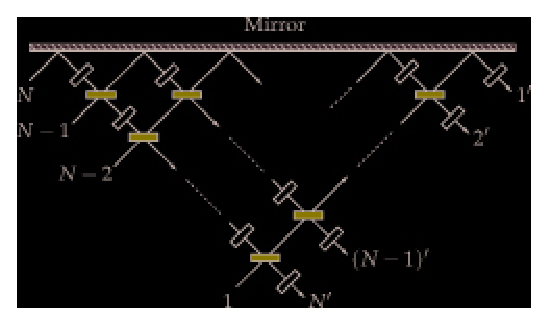
\includegraphics[width=8.5cm,height=8.5cm]{fig1-coherent}

\protect\caption[\hspace{1cm}NxN interferometer]{}


\label{coherent}
\end{figure}


%%%%%%%%%%%%%%%%%%%%%%%%%%%%%%%%%%%%%%%%%%%%%%%%
%%%%%%%%%%%%%%%%%%%%%%%%%%%%%%%%%%%%%%%%%%%%%%%%
%%%%%%%%%%%%%%%%%%%%%%%%%%%%%%%%%%%%%%%%%%%%%%%%
%%%%%%%%%%%%%%%%%%%%%%%%%%%%%%%%%%%%%%%%%%%%%%%%
\chapter*{Appendix 2: Lagrange Multipliers}

In our works we have relied quite heavily on the method of Lagrange
multipliers when optimizing a function which was under the restriction
of a constraint. We now show how it works \cite{Barnett2009}. The
method can be applied to a function of any number of variables but
it can be more clearly explained in two variables. Suppose that we
need to find the stationary points of a function $f(x,y),$ where
$x$ and $y$ are the two variables, subject to the constraint $g(x,y)=0.$
If the constraint is simple then we can solve for $x$ in terms of
$y,$ plug it into the function and solve $\partial f/\partial y=0.$
However for a more complicated constraint this can easily lead to
a very high order equation with cannot be solved analytically. In
the case of exact cloning, doing just so leads to a sixth order equation
which is of little use. 

To find the stationary points of a function of two variables such
as $f(x,y),$ we could just take the total differential $df$ and
set it to zero

\begin{equation}
df=\frac{\partial f}{\partial x}dx+\frac{\partial f}{\partial y}dy=0,\label{eq:lagrange 1}
\end{equation}
which leads to two conditions:

\begin{equation}
\frac{\partial f}{\partial x}=0,\ \ \frac{\partial f}{\partial y}=0.\label{eq:lagrange 0}
\end{equation}


However there is a constraint which means that the differentials $dx$
and $dy$ are not independent, they are related to the total differential
of $g$ by:

\begin{equation}
dg=\frac{\partial g}{\partial x}dx+\frac{\partial g}{\partial y}dy=0.\label{eq:lagrange 2}
\end{equation}


Multiplying (\ref{eq:lagrange 2}) by the Lagrange parameter $\lambda$
and adding it to (\ref{eq:lagrange 1}) we get 

\begin{equation}
d(f+\lambda g)=(\frac{\partial f}{\partial x}+\lambda\frac{\partial g}{\partial x})dx+(\frac{\partial f}{\partial y}+\lambda\frac{\partial g}{\partial y})dy
\end{equation}


This equation can be satisfied by choosing the Lagrange multiplier
$\lambda$ such that the following two conditions are satisfied:

\begin{equation}
\frac{\partial f}{\partial x}+\lambda\frac{\partial g}{\partial x}=0\label{eq:lagrange x}
\end{equation}


and

\begin{equation}
\frac{\partial f}{\partial y}+\lambda\frac{\partial g}{\partial y}=0\label{eq:lagrange y}
\end{equation}


To get the stationary points of $f(x,y)$ follow this procedure:
\begin{itemize}
\item Solve the two equations: (\ref{eq:lagrange x}) and (\ref{eq:lagrange y})
in terms of $\lambda,$ $x(\lambda)$ and $y(\lambda)$; 
\item Plug $x(\lambda)$ and $y(\lambda)$ into the constraint $g(x,y)$
;
\item Solve for $\lambda$; 
\item Plug the value of $\lambda$ into $x(\lambda)$ and $y(\lambda)$; 
\item Plug $x(\lambda)$ and $y(\lambda)$ into the function which was to
be optimized $f(x,y)$.
\end{itemize}
Now that we have seen how the Lagrange multipliers method works, we
can simplify the procedure by optimizing the function following function:

\begin{equation}
F(x,y)=f(x,y)+\lambda g(x,y)\label{eq:lagrange full}
\end{equation}
with respect to the the independent variable $x$ and $y.$ Differentiating
(\ref{eq:lagrange full}) with respect to $x$ and $y,$ we obtain
equations (\ref{eq:lagrange x}) and (\ref{eq:lagrange y}). The rest
of the procedure is the same. This is the exact procedure we used
for our works, for example in optimizing the error rate $P_{E}(r_{1},r_{2})$
with one constraint $s(r_{1},r_{2}).$ 



\bibliographystyle{unsrt}
\bibliography{/Users/ashehu/Desktop/mendeley}

\end{document}
